%%%%%%%%%%%%%%%%%%%%%%%%%%%%%%%%%%%%%%%%%%%%%%%%%%%%%%%%%%%%%%%%%%%%%%%%%%%%%%%%%%%%%%%%%%%
%%
%% CCRMS Dissertation - Cross-Chain Content Rights Management Service
%% Based on University of Malta CDLT LaTeX Template
%% https://github.com/jp-um/university_of_malta_LaTeX_dissertation_template
%%
%%%%%%%%%%%%%%%%%%%%%%%%%%%%%%%%%%%%%%%%%%%%%%%%%%%%%%%%%%%%%%%%%%%%%%%%%%%%%%%%%%%%%%%%%%%

%% ======================================================================
%% Build entry point for the dissertation.
%%
%% Structure (in order of output):
%%   frontmatter  copyright, originality, acknowledgements, abstract,
%%                table of contents, list of tables, list of abbreviations
%%   mainmatter   Chapters 1-9 (chap1/...chap9/)
%%   appendix     Appendices A-F (appA/...appF/)
%%   backmatter   bibliography (references.bib, \nocite{*} includes all
%%                100 entries with ragged-right layout)
%%
%% Build sequence (required for full cross-reference + citation resolve):
%%   pdflatex dissertation_main
%%   bibtex   dissertation_main
%%   pdflatex dissertation_main
%%   pdflatex dissertation_main
%%
%% Or: latexmk -pdf dissertation_main (does the above automatically).
%%
%% Key customizations added to the stock CDLT template:
%%   - microtype package (better line-breaking)
%%   - \setlength{\emergencystretch}{3em} (prevents margin overflow when
%%     long \texttt{} tokens cannot break at sensible points)
%%   - \newcolumntype{L}{} and \newcolumntype{R}{} for ragged-right /
%%     ragged-left fixed-width table columns (avoids \texttt{}
%%     justification stretching in long tables)
%%   - \raggedright inside the bibliography block (URLs don't justify well)
%%   - \nocite{*} includes every bib entry in the final bibliography,
%%     matching the lit-review source count of 100 unique entries
%%   - \listoffigures* restored (seven TikZ diagrams: four in Chapter 4,
%%     one each in Chapters 5, 6, and 7)
%%
%% Metadata (title, author, ID, supervisor, degree, date) is set below in
%% the "(Your) Data" block. Verify these before submission.
%% ======================================================================

\RequirePackage[l2tabu, orthodox]{nag}

\documentclass[twoside]{um}


%% **************** (Your) Packages (Start) ******************

\usepackage{booktabs}       % professional tables (\toprule, \midrule, \bottomrule)
\usepackage{longtable}      % tables spanning multiple pages
\usepackage{array}          % extra column formatting
\usepackage{listings}       % code listings
\usepackage{xcolor}         % colored code
\usepackage{textcomp}       % additional text symbols
\usepackage{hyperref}       % clickable cross-references
\usepackage{microtype}      % better line-breaking / character protrusion
\usepackage{tikz}           % diagrams (architecture, NFT nesting, XCM flow, three models)
\usetikzlibrary{arrows.meta, positioning, fit}
\usepackage[font=small,labelfont=bf,labelsep=period]{caption} % distinct caption style

% Allow LaTeX more flexibility to stretch lines that contain long unbreakable
% \texttt{} tokens (code identifiers, hex addresses). Without this, long tokens
% overflow into the margin rather than causing an earlier line break.
\setlength{\emergencystretch}{3em}

% Pin floats to the top of float-only pages instead of vertically centering them.
\makeatletter
\setlength{\@fptop}{0pt}
\makeatother

% Custom left-aligned (ragged-right) fixed-width column for text-heavy tables.
% Use L{0.25\linewidth} instead of p{0.25\linewidth} to avoid justification stretching.
\newcolumntype{L}[1]{>{\raggedright\arraybackslash}p{#1}}
% Right-aligned fixed-width counterpart, for numeric columns that would otherwise
% auto-expand beyond the text block when their header is wide.
\newcolumntype{R}[1]{>{\raggedleft\arraybackslash}p{#1}}

% Code listing style
\lstdefinestyle{code}{
    basicstyle=\ttfamily\footnotesize,
    breaklines=true,
    frame=single,
    numbers=left,
    numberstyle=\tiny\color{gray},
    keywordstyle=\color{blue},
    commentstyle=\color{green!50!black},
    stringstyle=\color{red!60!black},
    showstringspaces=false,
    tabsize=2
}
\lstset{style=code}

%% ***************** (Your) Packages (End) *******************


%% **************** (Your) Data (Start) ******************

\title{Cross-Chain Content Rights\\Management Service}
\tagline{A Polkadot-Based Unified Rights Token for Subscription,\\Pay-Per-View, and Permanent Ownership}
\author{Ryc Brownrigg}
\authorID{2104001}
\supervisor{Dr Joshua Ellul}
%%\cosupervisor{Dr Someone}                              %% uncomment if applicable
\department{Centre for Distributed Ledger Technologies}
\faculty{Faculty of ICT}
\degree{M.Sc.\ in Blockchain and Distributed Ledger Technologies (ICT)}
\doctype{dissertation}
\degreedate{July, 2026}

%% ***************** (Your) Data (End) *******************


%% ******** (Your) Document Settings (Start) *************

\graphicspath{{./images/}}

%% ********* (Your) Document Settings (End) **************


\begin{document}
\frontmatter
    \maketitle
    %% ======================================================================
%% frontmatter/copyright.tex
%%
%% Copyright page.
%%
%% The file body is intentionally minimal -- the um.cls template defines
%% the copyrightenv environment (see um.cls ~line 293) to automatically
%% render the UM logo, "Copyright (c) <year> University of Malta",
%% www.um.edu.mt, and the first-edition date. No authored content is
%% needed in this file; just invoking the environment is sufficient.
%% ======================================================================

\begin{copyrightenv}
\end{copyrightenv}

    %% ======================================================================
%% frontmatter/originality.tex
%%
%% Statement of Originality (CDLT-mandated Declaration by Postgraduate
%% Students).
%%
%% The file body is intentionally minimal -- the um.cls template defines
%% the originality environment (see um.cls ~line 248) to automatically
%% render the official declaration text: (a) Authenticity of
%% Dissertation and (b) Research Code of Practice and Ethics Review
%% Procedures. No authored content is needed here; invoking the
%% environment emits the full mandated statement.
%% ======================================================================

\begin{originality}
\end{originality}
    %% ======================================================================
%% frontmatter/acknowledgements.tex
%%
%% Acknowledgements.
%%
%% Five paragraphs thanking, in order: supervisor (Prof. Ellul),
%% faculty (Centre for DLT), external communities (Polkadot /
%% Kusama, Parity Technologies' Canary Chaos program), writing and
%% dictation tooling (Grammarly, SuperWhisper), and family (mother).
%% ======================================================================

\begin{acknowledgements}

I express my deepest gratitude to my supervisor, Dr Joshua Ellul, for his insightful guidance, patience, and unwavering support throughout this dissertation.

I am also grateful to the faculty of the Centre for Distributed Ledger Technologies for creating the academic environment in which this work was produced.

To the Polkadot and Kusama communities for their documentation, tooling, and open-source contributions that supported this work. We also thank Parity Technologies for the Polkadot SDK, comprehensive documentation, and tooling that made this implementation feasible.

I am particularly grateful to Grammarly, which served as an indispensable tool for grammar, spelling, clarity, and rephrasing throughout the writing and revision process. I am also grateful to SuperWhisper, the dictation software that allowed me to compose most of this dissertation by voice rather than typing, making the writing process far more accessible and efficient given my limited typing speed.

Finally, I want to thank my mother, whose endless love, encouragement, and faith in me have carried me through all my wild and wonderful adventures. I love you so much, Mom.

Thank you all.

\end{acknowledgements}

    %% ======================================================================
%% frontmatter/abstract.tex
%%
%% Abstract (and keywords).
%%
%% Structured as five paragraphs: (1) generic problem and gap,
%% (2) Polkadot justification and research question,
%% (3) system description and evaluation method, (4) results,
%% (5) three principal findings.
%%
%% Written in third person per CDLT guidelines (abstract must not use
%% first person). No citations or footnotes per guidelines.
%% Target ≤300 words; actual length approx. 295 words.
%% ======================================================================

\begin{abstract}

The content creator economy concentrates value in centralized intermediaries. No existing system, centralized or decentralized, provides subscription access, pay-per-view consumption, and permanent ownership through a single rights primitive that is portable across heterogeneous blockchain networks.

Polkadot's architecture is well-suited to investigate this gap. Its relay chain provides shared validator security, removing the external trust assumptions inherent in bridge-based solutions; XCM natively carries rights-management operations between parachains through a standardized protocol; and FRAME's composable module system allows subscription, pay-per-view, and permanent-ownership logic to coexist within a single runtime unit. This dissertation asks: \textit{how can a shared-security, multi-chain framework built on Polkadot XCM and FRAME primitives deliver a unified rights record natively supporting all three monetization models across heterogeneous blockchain networks, and what levels of transaction finality, cost efficiency, and creator revenue retention can it achieve?}

The Cross-Chain Content Rights Management Service (CCRMS) is a Polkadot parachain prototype designed to address this question. It has been evaluated through unit testing, performance benchmarks, a security audit, a centralized baseline comparison, and a Monte Carlo creator-revenue simulation.

The prototype achieves 26.2 transactions per second at a 96.9\% inclusion rate in the happy-path window of the stress test (Section~\ref{subsec:stress-test}), approximately six-second inclusion latency, and a destination-chain inclusion delay of up to seven blocks (median 5, approximately 30--35~s). The economic simulation yields approximately 16.8\% higher average creator revenue than centralized platforms, though this advantage is highly audience-dependent: creators above approximately 10,000 followers benefit decisively, whereas those below approximately 3,600 are better served by centralized discovery platforms. This result characterizes the CCRMS design; the benchmarked prototype bounds the number of rights holders per content item, which must be lifted before the advantage can be realized for larger audiences.

Three findings advance the state of knowledge. First, a unified rights record supporting all three access models can be built from standard FRAME primitives without novel cryptographic mechanisms, closing literature gap G7. Second, the revenue advantage of decentralized rights management is not universal, crossing a follower threshold at approximately 3,600. Third, conservative architectural choices provided resilience against an ecosystem-level disruption that occurred during the implementation period.

\end{abstract}

\noindent\textbf{Keywords:} cross-chain content rights, Polkadot XCM, unified rights record, creator revenue retention, design science research
\if@openright\cleardoublepage\else\clearpage\fi
    \tableofcontents*\if@openright\cleardoublepage\else\clearpage\fi
    \listoftables*\if@openright\cleardoublepage\else\clearpage\fi
    \listoffigures*\if@openright\cleardoublepage\else\clearpage\fi
    %% ======================================================================
%% frontmatter/abbreviations.tex
%%
%% List of Abbreviations.
%%
%% 50 entries, alphabetised, rendered as a longtable (two columns:
%% abbreviation in bold, full expansion). Uses \chapter* to avoid
%% auto-numbering but adds a manual ToC entry via \addcontentsline.
%% Entry set reflects advisor-approved filtering: ID, GB, USD, BLS, DOT
%% kept despite being common; IP and HOL removed.
%% ======================================================================

\chapter*{List of Abbreviations}
\markboth{List of Abbreviations}{List of Abbreviations}
\addcontentsline{toc}{chapter}{List of Abbreviations}

\begin{longtable}{@{}L{0.18\linewidth} L{0.78\linewidth}@{}}
\textbf{ABI} & Application Binary Interface \\
\textbf{AI} & Artificial Intelligence \\
\textbf{API} & Application Programming Interface \\
\textbf{ASCII} & American Standard Code for Information Interchange \\
\textbf{BLS} & Boneh--Lynn--Shacham (signature scheme) \\
\textbf{CAGR} & Compound Annual Growth Rate \\
\textbf{CCRMS} & Cross-Chain Content Rights Management Service \\
\textbf{CLI} & Command-Line Interface \\
\textbf{CPU} & Central Processing Unit \\
\textbf{DEX} & Decentralized Exchange \\
\textbf{DOT} & Polkadot native token \\
\textbf{DRM} & Digital Rights Management \\
\textbf{DSR} & Design Science Research \\
\textbf{ESMA} & European Securities and Markets Authority \\
\textbf{ETH} & Ether (Ethereum's native token) \\
\textbf{EU} & European Union \\
\textbf{EVM} & Ethereum Virtual Machine \\
\textbf{FRAME} & Framework for Runtime Aggregation of Modularized Entities \\
\textbf{GB} & Gigabyte \\
\textbf{H160} & 160-bit hash (Ethereum-style address) \\
\textbf{HHI} & Herfindahl-Hirschman Index \\
\textbf{HRMP} & Horizontal Relay-routed Message Passing \\
\textbf{HTTP} & Hypertext Transfer Protocol \\
\textbf{ID} & Identifier \\
\textbf{IPFS} & InterPlanetary File System \\
\textbf{JAM} & Join-Accumulate Machine \\
\textbf{JSON} & JavaScript Object Notation \\
\textbf{KPI} & Key Performance Indicator \\
\textbf{MEV} & Maximal Extractable Value \\
\textbf{MiCA} & Markets in Crypto-Assets (EU Regulation) \\
\textbf{MTTR} & Mean Time To Recovery \\
\textbf{NFT} & Non-Fungible Token \\
\textbf{OTT} & Over-The-Top (media service) \\
\textbf{PIL} & Programmable IP License (Story Protocol) \\
\textbf{PolkaVM} & Polkadot Virtual Machine \\
\textbf{PPV} & Pay-Per-View \\
\textbf{RISC} & Reduced Instruction Set Computer \\
\textbf{RMRK} & Remark (NFT protocol; derived from the \texttt{system.remark} extrinsic) \\
\textbf{RPC} & Remote Procedure Call \\
\textbf{SCALE} & Simple Concatenated Aggregate Little-Endian (Substrate codec) \\
\textbf{SDK} & Software Development Kit \\
\textbf{SIGTERM} & Signal Terminate (POSIX signal) \\
\textbf{SQL} & Structured Query Language \\
\textbf{TLS} & Transport Layer Security \\
\textbf{TPS} & Transactions Per Second \\
\textbf{TVL} & Total Value Locked \\
\textbf{UI} & User Interface \\
\textbf{USD} & United States Dollar \\
\textbf{WASM} & WebAssembly \\
\textbf{XCM} & Cross-Consensus Messaging \\
\textbf{ZK} & Zero-Knowledge (proof / cryptography) \\
\end{longtable}
\if@openright\cleardoublepage\else\clearpage\fi

\pagestyle{umpage}
\mainmatter
    %% ======================================================================
%% chap1/introduction_main.tex
%%
%% Chapter 1: Introduction
%%
%% Opens the dissertation: states the problem, gives background context,
%% introduces the research aim and approach, lists contributions, and
%% acknowledges scope and limitations.
%%
%% Sections:
%%   1.1 The Problem
%%   1.2 Background Context
%%   1.3 Research Aim and Approach
%%   1.4 Contributions
%%   1.5 Scope and Limitations
%%
%% External labels referenced:
%%   chap:background (Ch 2), chap:research-questions (Ch 3),
%%   chap:methodology (Ch 4), chap:evaluation (Ch 6),
%%   chap:results (Ch 7), chap:discussion (Ch 8),
%%   chap:conclusion (Ch 9), sec:summary-of-contributions (9.1),
%%   sec:research-objectives (3.3),
%%   sec:ink-discontinuation (Appendix A.9)
%%
%% Citations: dengEtAl2025, liEtAl2025a, hevnerEtAl2004
%% ======================================================================

\chapter{Introduction}\label{chap:introduction}

\section{The Problem}\label{sec:the-problem}

The prevailing content economy is unfavorable to creators. An independent musician earning USD~100,000 in streaming revenue typically retains between USD~55,000 and USD~70,000 after platform fees and distributor commissions --- a figure that falls substantially lower for label-signed artists \citep{musicBizResearch2024}. Centralized intermediaries retain between 30 and 60 percent of gross creator revenue, varying by platform and contract structure; the per-platform breakdown used in our analysis is presented in Section~\ref{subsec:fee-analysis} (Table~\ref{tab:fees}). Fees are non-negotiable, audiences are non-portable, and content rights remain bound by the platform's terms of service throughout.

Consumers face analogous fragmentation. A film bought on iTunes cannot be streamed on Amazon Prime; an Audible audiobook cannot be transferred to Google Play; a subscription started on one platform cannot move to another. Consumers do not own their purchases; they hold a platform-bound license that can be revoked, modified, or ignored. The fragmentation that constrains creators also restricts the consumers who support them.

Fragmentation extends to monetization models. Subscriptions typically live on Patreon; one-time sales on Gumroad; pay-per-view is scarcely supported at all, because the overhead of conventional payment systems makes micro-transactions uneconomic. Each platform supports one monetization model, holds its own audience, takes its own fees, and produces its own accounting reports. A creator who wants to offer all three models is forced to run three or four platforms in parallel and reconcile them by hand.

Existing blockchain alternatives address parts of the problem but not the whole. Non-fungible tokens (NFTs) provide transferable ownership but not recurring access or per-view consumption. Subscription-style decentralized platforms (such as Audius) offer recurring revenue but are confined to a single chain and audience. Cross-chain bridges move assets between ecosystems but lack rights metadata. Blockchain-based digital rights management has been examined in the academic literature specifically for the music industry \citep{cirelloEtAl2023}, with proposed solutions sharing a common limitation: they address rights metadata or royalty distribution in isolation, without combining all three monetization models into a single portable primitive. No existing system, centralized or decentralized, delivers subscription, pay-per-view, and permanent ownership from a single rights primitive portable across blockchains.

The technical primitives to resolve this (cross-chain messaging, programmable smart contracts, on-chain royalty distribution, and NFT-based rights tokenization) all exist as standalone capabilities. Hanneke et al.\ \citeyearpar{hannekeEtAl2024} characterize this class of systems as an emerging \emph{Internet of Value}, in which blockchain tokenization enables asset ownership and revenue flows that bypass centralized intermediaries entirely. Our research examines whether these primitives can be integrated into a coherent system that benefits creators over existing solutions, and the conditions under which creators would adopt it.

\section{Background Context}\label{sec:background-context}

This dissertation sits at the intersection of three research and engineering areas: blockchain-based digital rights management, cross-chain interoperability, and decentralized content monetization. Each is surveyed in Chapter~\ref{chap:background}; this section gives the context needed to motivate the work.

The global Digital Rights Management market is large and growing. Independent estimates from MarketsandMarkets, Mordor Intelligence, and Grand View Research place it at approximately USD~6.7~billion in 2025, forecast to reach USD~11--14~billion by 2030 (10--11\% CAGR), driven by streaming services, OTT platforms, rising AI-related piracy, and regulatory pressure. The blockchain-specific segment is smaller but expanding at approximately 33\% annually, projected to reach USD~2.74~billion by 2030.

Cross-chain interoperability has emerged as an active research area during the implementation window. A 2023 survey in IEEE Transactions on Knowledge and Data Engineering \citep{renEtAl2023} classifies interoperability approaches into five categories --- sidechains, notary schemes, hashed time lock contracts, relays, and blockchain-agnostic protocols --- and two further 2025 surveys \citep{dengEtAl2025, liEtAl2025a} collectively cover more than 150 sources. The Polkadot ecosystem that underpins our technical foundation completed its 2.0 upgrade during this period, introducing Async Backing, Agile Coretime, and Elastic Scaling. These features materially improve per-parachain latency and throughput. Snowbridge, the trust-minimized Polkadot--Ethereum bridge, launched V2 in November 2025 with USD~75~million in total value locked. JAM, Polkadot's next-generation relay-chain architecture, reached testnet in January 2026.

In January 2026, the ink! Alliance discontinued development of ink!, the language chosen for the CCRMS contract layer; our pallet-first architecture proved resilient to the change (Appendix~\ref{sec:ink-discontinuation}). The EU AI Act copyright provisions (August 2025) and MiCA (full enforcement July 2026) create regulatory demand for cryptographic provenance and tamper-evident rights records, functions that CCRMS can provide.

\section{Research Aim and Approach}\label{sec:research-aim-and-approach}

Our objective is to \textbf{design, implement, and evaluate a functional prototype of a cross-chain content rights management service that supports three monetization models: subscription, pay-per-view, and permanent ownership, using a single unified rights primitive with automatic royalty distribution and cross-chain portability}. We designate this prototype as CCRMS (the Cross-Chain Content Rights Management Service) and implement it as a Polkadot parachain.

The primary research question that guides our work is:

\begin{quote}
How can a shared-security, multi-chain framework built on Polkadot's Cross-Consensus Messaging (XCM) and FRAME pallet primitives deliver a unified rights token that natively supports recurring subscriptions, pay-per-view microtransactions, and permanent ownership transfers across heterogeneous blockchain networks, and what levels of transaction finality, cost efficiency, and creator revenue retention can such a system achieve?
\end{quote}

The question comprises two distinct components: a \textbf{design feasibility} question (assessing whether the system can be constructed using available primitives) and a \textbf{measurement} question (determining the system's operational properties and comparing them to alternative options). We treat these components as mutually constraining and report their results relative to one another. A comprehensive statement of the primary question, the five sub-questions that decompose it, and the six research objectives addressing them is presented in Chapter~\ref{chap:research-questions}.

Our research approach is grounded in \textbf{design science research} \citep{hevnerEtAl2004} as applied to a multi-component blockchain prototype. We organize the methodology, detailed in Chapter~\ref{chap:methodology}, into iterative build-test-measure-refine cycles within a six-phase framework. Our evaluation strategy, as delineated in Chapter~\ref{chap:evaluation}, combines quantitative measures, including technical benchmarks, security audits, comparative analyses, and Monte Carlo simulations of creator revenue, with qualitative insights from literature synthesis. We frame the evaluation as \textbf{measurement-focused} rather than target-driven: our objective is to document and analyze the levels of performance, security, and economic viability achieved by the system, rather than to verify conformity with a predefined set of criteria.

\section{Contributions}\label{sec:contributions}

We make contributions across four categories, described in detail in Section~\ref{sec:summary-of-contributions}:

\begin{enumerate}
\item \textbf{A working artifact:} the CCRMS parachain implementation (Rust, ink!, and JavaScript), released as open source under the MIT license.
\item \textbf{Formal documentation:} seven implementation specifications that explain what the artifact does and why each design decision was made.
\item \textbf{Empirical findings:} technical performance measurements, a Monte Carlo creator-revenue result (CCRMS produces higher mean revenue, strongly conditional on audience size), and eight security audit findings, of which one Medium and one Low were remediated.
\item \textbf{A worked example} of applying design science research to a multi-component blockchain prototype, a combination seldom exemplified in existing DSR literature.
\end{enumerate}

\section{Scope and Limitations}\label{sec:scope-and-limitations}

This dissertation is bound in several ways that the reader should be aware of prior to engaging with the main content chapters.

\textbf{The prototype is a back-end service, not a consumer application.} We did not develop a web or mobile interface for CCRMS. Our assessment focuses on pallet- and runtime-level behavior; we do not directly evaluate user-experience factors. We recognize this as a limitation in Chapters~\ref{chap:evaluation} and~\ref{chap:discussion} and as an area for future research in Chapter~\ref{chap:conclusion}.

\textbf{We take the measurements on a local development network.} Our CCRMS prototype runs in a local Zombienet topology with two relay-chain validators and single-collator parachains. In production, parachains are hosted on the Polkadot or Kusama relay chains, which have hundreds of validators, real-world network latency, and competition from many other parachains. The throughput, latency, and reliability metrics in Chapter~\ref{chap:results} should be treated as \textbf{upper bounds for the test environment}, not forecasts of real-world deployment performance.

\textbf{Our Snowbridge integration uses a local Ethereum stack.} We successfully demonstrated the bridge with two transactions, each for one ETH, bridging from a local Ethereum chain to a local AssetHub parachain. However, the entire configuration remains local; no public testnet or mainnet has been used. This integration serves as a proof of architectural feasibility rather than a production validation.

\textbf{We have not commissioned any third-party audit, security review, or independent benchmarking.} A single author performed the implementation, test design, measurements, and interpretation in this dissertation. Deployment to production would require third-party validation before any substantive value is processed.

\textbf{We did not fully achieve two of the six research objectives.} RO5 (zero-knowledge proof hooks for selective regulatory disclosure) was not undertaken. The complexity of integrating a ZK proof system into a Substrate runtime, selecting a proof system, building or adopting a verifier pallet, designing the selective disclosure protocol, and producing testable proof-of-concept circuits was substantially greater than the original Phase~2 objective anticipated. We acknowledge the underestimate. RO2 (off-chain indexing) was partially implemented: the pallet's emitted events are sufficient for direct on-chain queries, but we did not deploy a separate indexer (e.g., SubQuery). We document both omissions in Chapter~\ref{chap:research-questions}, Section~\ref{sec:research-objectives}, and revisit them as future work in Chapter~\ref{chap:conclusion}.
             % Chapter 1: Introduction
    %% ======================================================================
%% chap2/background_main.tex
%%
%% Chapter 2: Background and Related Work
%%
%% Surveys scholarly and industry publications across four themes:
%% blockchain-based content management, cross-chain interoperability,
%% decentralized monetization models, and the gaps that motivate the
%% research. Closes with Table 2.1 mapping eight identified gaps to
%% CCRMS contributions.
%%
%% Sections:
%%   2.1 Blockchain-Based Content Management (3 subsections)
%%   2.2 Cross-Chain Interoperability (5 subsections)
%%   2.3 Decentralized Monetization Models (6 subsections)
%%   2.4 Challenges and Gaps (Table 2.1 -- literature gaps and CCRMS
%%       contributions)
%%   2.5 Summary
%%
%% External labels referenced:
%%   subsec:ink-contract (5.2.4), subsec:royalty-propagation (5.2.3),
%%   subsec:comparative-analysis (7.1.7),
%%   subsec:decentralization-hhi (7.3.3),
%%   sec:ink-discontinuation (Appendix A.9)
%%
%% Citations: extensive -- approximately two-thirds of references.bib,
%% spanning DRM, cross-chain surveys, NFT/IP rights, monetization models,
%% smart contracts, the Polkadot ecosystem, and EU regulatory frameworks.
%% See in-line \citep{} and \citet{} commands for specific keys.
%% ======================================================================

\chapter{Background and Related Work}\label{chap:background}

This chapter surveys four themes: blockchain-based content management (Section~\ref{sec:blockchain-content-management}), cross-chain interoperability (Section~\ref{sec:cross-chain-interop}), decentralized monetization models (Section~\ref{sec:decentralized-monetization}), and the challenges and gaps that motivate the research (Section~\ref{sec:challenges-and-gaps}).

\section{Blockchain-Based Content Management}\label{sec:blockchain-content-management}

\subsection{Market Context}\label{subsec:market-context}

Three independent market research firms \citep{marketsandMarkets2025, mordorIntelligence2026, grandViewResearch2025} converge on estimates that the global DRM market is valued at approximately USD~6.7--6.9~billion in 2025--2026, with projections reaching USD~11--14~billion by 2030--2033, representing a Compound Annual Growth Rate (CAGR) of 10--11\%. This growth is primarily driven by streaming services, AI-enabled piracy, and regulatory pressures. The market is dominated by \textbf{content protection} solutions (such as Widevine, FairPlay, PlayReady), rather than \textbf{content monetization}.

\subsection{Foundational Work on Blockchain-Based DRM}\label{subsec:foundational-drm}

Blockchain-based Digital Rights Management (DRM) is an active research domain. \citet{garbaEtAl2021} incorporate digital watermarking into blockchain technology as a tamper-evident layer; \citet{patilEtAl2022} build on this by introducing the DRMChain hybrid encryption architecture; and \citet{yiEtAl2023} further extend the protection model with a redactable blockchain scheme that combines DRM with perceptual hashing, enabling selective content modification without invalidating ownership proofs. Both earlier studies prioritize protection mechanisms over the economics of content creators.

In the music industry, \citet{cirelloEtAl2023} derive a set of design principles for blockchain-based DRM systems through expert interviews and prototype testing, identifying transparency of rights ownership, automated royalty distribution, and programmable licensing as the three foundational requirements. \citet{cherdakovEtAl2023} and \citet{mendozaTelloEtAl2024} propose Web3 implementations that embed these principles in music-streaming smart contracts, demonstrating the feasibility of on-chain licensing but stopping short of cross-chain portability.

The most comprehensive recent work is \citet{madapatiPradhan2025}, whose Ethereum + IPFS framework achieves 409~TPS for registration; this comparison is misleading because their pipeline hashes off-chain and stores only results on-chain. \citet{wangEtAl2025} present a BLS threshold signature scheme achieving 40\,ms aggregation. Two Polkadot-specific studies \citep{xieLiu2022, xieTang2024a} propose conceptual cross-chain frameworks without working prototypes.

This literature establishes \textbf{blockchain-based DRM as a legitimate research domain}; its consistent limitation is that it emphasizes protection over monetization, a priority CCRMS reverses.

\subsection{NFTs and Intellectual Property Rights}\label{subsec:nfts-ip-rights}

Work on NFTs and intellectual property encompasses legal analysis \citep{uspto2024, davik2025, murray2022, eurojust2024} and standardization proposals \citep{reggianini2025, gattoEtAl2021, dreyerEtAl2021}. The most empirically significant study is \citet{darshanEtAl2025}: \textbf{80\% of mainstream NFTs fail to transfer copyright, only 12--30\% of listings include licensing information, and 50--60\% of secondary sales bypass creator royalties}. \citet{lahiriEtAl2026} confirm these findings via a meta-analysis of 125 NFT studies, identifying legal clarity around ownership transfers as the field's primary unsolved problem. \citet{cabotNadalEtAl2022} propose an ERC-721 extension enabling recipients to reject unwanted transfers, relevant to our permanent-ownership mode.

The most significant industry development is the February 2025 launch of \textbf{Story Protocol}, the first dedicated intellectual-property Layer-1 blockchain \citep{storyFoundation2025}. Built on the Cosmos SDK with EVM compatibility, it enables programmable IP registration, automated licensing, and on-chain royalty distribution. It is the most direct industry comparator to CCRMS: a single-chain L1 versus a cross-chain parachain.

\section{Cross-Chain Interoperability}\label{sec:cross-chain-interop}

\subsection{Polkadot Architecture}\label{subsec:polkadot-architecture}

Polkadot \citep{wood2016} is a heterogeneous multi-chain framework in which parachains share security through a central relay chain and communicate via XCM. The core primitives are parachains, the relay chain, validators, collators, and XCM. \citet{habermeierEtAl2021} and \citet{wood2022} provide the primary technical documentation for the XCM message format and multi-hop features that underpin our cross-chain implementation. The XCM protocol itself has received dedicated academic attention: \citet{morhacEtAl2023a} build ParaSpell, a developer SDK that abstracts XCM message construction across parachains, and \citet{morhacEtAl2023b} demonstrate XCMP interoperability at the protocol level. Together with \citet{morhacEtAl2025}, which proposes the Unispell universal adapter, they form the most coherent body of peer-reviewed academic work on XCM in practice.

Bridge-based systems such as Wormhole and LayerZero rely on external validator committees that could be compromised independently, enabling forged ownership proofs or hijacked royalty distributions. Polkadot's shared-security model eliminates this risk: all parachains use the same relay-chain validator set. Cross-chain rights operations use HRMP, which routes messages through the relay chain and inherits its security and finality.

\subsection{Cross-Chain Technology Surveys}\label{subsec:cross-chain-surveys}

The cross-chain literature matured rapidly from 2022 to 2025. \citet{renEtAl2023} classify interoperability solutions into five categories: sidechains, notary schemes, hashed time lock contracts, relays, and blockchain-agnostic protocols. \citet{maoEtAl2022} provide an earlier three-category taxonomy; \citet{bigiottiEtAl2025} extend both in ACM Computing Surveys. Two more recent surveys expand the field: \textbf{\citet{dengEtAl2025}} analyze more than 150 sources; \textbf{\citet{liEtAl2025a}} distinguish \textbf{asset interoperability} (token transfers) from \textbf{data interoperability} (cross-chain state verification). The latter distinction is directly relevant: CCRMS addresses both through XCM payments and \texttt{pallet-rights-verifier} Merkle proofs. \citet{kumarVEtAl2025} and \citet{caoEtAl2025} examine cross-chain efficiency and trustless interoperability, both aligned with CCRMS's design intent.
\subsection{Bridges and Snowbridge}\label{subsec:bridges-snowbridge}

Bridge architecture research includes \citet{yinEtAl2022} on multi-party computation, \citet{chenKEtAl2023} on reputation-based trust, and \citet{maricEtAl2025} on Isabelle/HOL formal verification of fail-safe bridges.

The most operationally significant development in blockchain infrastructure is \textbf{Snowbridge}, a trust-minimized bridge that enables interoperability between Polkadot and Ethereum. Snowbridge V2 was officially launched on the Polkadot mainnet on November 7, 2025, and includes support for arbitrary Ethereum contract calls from Polkadot, a 50\% fee reduction, and unordered message execution \citep{snowfork2025a}. The associated Polkassembly proposal \citep{snowfork2025b} documents more than a year of operational stability with no on-chain downtime. We position our Snowbridge integration as forward-compatible with V2, even though we developed the initial prototype against V1.

\subsection{Polkadot 2.0 and JAM}\label{subsec:polkadot-2-jam}

Two major ecosystem developments shaped our implementation timeline. \textbf{Polkadot 2.0} was comprehensively launched by October 2025, introducing Async Backing (eliminating relay-chain wait), Agile Coretime (on-demand block production), Elastic Scaling (multiple cores per parachain), and XCM v5 (multi-hop transactions) \citep{parityUpgrade2025, polkadotNetwork2025}. \textbf{JAM} (Join-Accumulate Machine, \citet{wood2024}) is expected to succeed the relay-chain model within the Polkadot ecosystem, with its testnet launched in January 2026 and mainnet scheduled for mid-to-late 2026. These developments confirm that the Polkadot architecture is \textbf{maturing rather than stagnating}.

\subsection{Cross-Chain Copyright Management as a Research Target}\label{subsec:cross-chain-copyright-research}

Numerous studies examine cross-chain copyright management as a research issue \citep{xieLiu2022, xieTang2024a, munsonEtAl2022, mareckova2024, oreroEtAl2023, buzu2021}; however, none have developed a functional end-to-end prototype. This gap, together with the architectural analysis above, motivates the selection of XCM and FRAME as the implementation substrate and justifies choosing Polkadot as the platform over single-chain or bridge-based alternatives.

XCM is preferred over Wormhole and LayerZero because it is native to the relay chain and introduces no additional trust assumptions. Its structured instruction format also encodes rights operations as typed, on-chain-interpretable messages rather than opaque byte payloads, preserving rights metadata across chain boundaries (gap~G3). FRAME is the implementation framework of choice over EVM and CosmWasm alternatives because its composable module system allows all three access modes to share a single pallet and access-check function, its weight benchmarking provides deterministic fee calculations, and its typed storage API exposes rights state as queryable on-chain objects via the RPC layer.

\section{Decentralized Monetization Models}\label{sec:decentralized-monetization}

\subsection{Creator Economy Context}\label{subsec:creator-economy-context}

\citet{communipass2026} forecasts the creator economy will exceed USD~280~billion by the end of 2026. The blockchain-specific segment is growing rapidly, from USD~499.52~million (2024) to USD~2.74~billion by 2030 \citep{iresearch3602025}, driven by creator dissatisfaction with centralized platforms and maturing blockchain infrastructure.

\subsection{DeFi and Web3 Foundations}\label{subsec:defi-web3}

The conceptual foundation for decentralized monetization lies in DeFi. \citet{gogelEtAl2021} present the canonical Wharton overview of the DeFi ecosystem, covering AMMs, lending, derivatives, and stablecoins; \citet{atzori2017} analyzes decentralized governance through a political economy lens; and \citet{busch2022} provides a technical overview of Web3 from the United States Congressional Research Service.

\subsection{Subscription, Pay-Per-View, and Purchase Models}\label{subsec:subscription-ppv-purchase}

Earlier work on blockchain subscription and pay-per-view models includes \citet{munson2019, khan2024, castweet2019, steem2025, banerjeeEtAl2020}. Most of these works examine blockchain incentives without addressing the micropayment problem. Two more recent works are particularly relevant: \textbf{\citet{osemwegie2025}} surveys decentralized media monetization (identifying the problems CCRMS targets but not proposing a working system), and \textbf{\citet{shah2025}} proposes a smart-contract framework for royalty distribution that is the closest to our royalty propagation design in the existing literature. CCRMS extends Shah's approach using a FRAME pallet with stronger atomicity guarantees. \citet{wamugo2024} provides empirical data on NFT adoption by media organizations in Kenya, demonstrating that blockchain monetization is under active consideration in emerging markets.

\subsection{Pay-Per-View and the Micropayment Problem}\label{subsec:ppv-micropayment}

Pay-per-view models have historically struggled on blockchain platforms because gas fees have often exceeded content costs. \citet{goyalEtAl2019} introduce Gringotts, a secure micropayment system, but do not address the core fee issue. \citet{chegenizadehEtAl2024} directly address the micropayment verification layer, proposing a multi-agent, privacy-preserving approach for resource-constrained offline devices that reduces per-transaction overhead through smart-contract batching; their work supports our strategic decision to model PPV as a counter rather than a sequence of individual on-chain transactions. \subsection{Smart Contracts as the Implementation Layer}\label{subsec:smart-contracts-impl}

Surveys of the smart contract literature \citep{ante2020, linEtAl2022, singhEtAl2024a, quanEtAl2024} establish the field as mature; Parity's ink! blog posts \citep{parityTechnologiesInk3_2022, parityTechnologiesInk_2022} were the primary technical references during implementation. The most consequential development is the \textbf{discontinuation of ink! in January 2026} \citep{inkAlliance2026}, discussed as gap G8 and in Appendix~\ref{sec:ink-discontinuation}.

\subsection{Royalty Automation}\label{subsec:royalty-automation}

Few peer-reviewed studies address on-chain royalty automation; \citet{shah2025} and \citet{reggianini2025} are the primary examples (discussed in Section~\ref{subsec:subscription-ppv-purchase}).

\section{Challenges and Gaps}\label{sec:challenges-and-gaps}

Table~\ref{tab:gaps} maps eight literature gaps to CCRMS contributions.

\begin{longtable}{@{}L{0.03\linewidth} L{0.27\linewidth} L{0.28\linewidth} L{0.36\linewidth}@{}}
\caption{Literature Gaps and CCRMS Contributions}\label{tab:gaps}\\
\toprule
\textbf{ID} & \textbf{Gap} & \textbf{Supporting literature} & \textbf{CCRMS contribution} \\
\midrule
\endfirsthead

\multicolumn{4}{l}{\emph{Table~\ref{tab:gaps} continued from previous page}}\\
\toprule
\textbf{ID} & \textbf{Gap} & \textbf{Supporting literature} & \textbf{CCRMS contribution} \\
\midrule
\endhead

\midrule
\multicolumn{4}{r}{\emph{Continued on next page}}\\
\endfoot

\bottomrule
\endlastfoot

G1 & Existing systems are protection-focused, not monetization-focused & \citet{garbaEtAl2021}; \citet{patilEtAl2022}; \citet{cirelloEtAl2023}; \citet{madapatiPradhan2025}; commercial DRM (Widevine, FairPlay, PlayReady) & Unified rights token with monetization as the primary design goal; protection becomes a secondary consequence of correct rights management. \\
\addlinespace
G2 & No native cross-chain recurring payments & Existing cross-chain protocols (XCM, Wormhole, LayerZero, Snowbridge) address one-time transfers; \citet{xieLiu2022, xieTang2024a} propose theoretical frameworks without recurring payments & On-chain \texttt{on\_initialize} block hook scheduler for automatic renewal. XCM v5 \texttt{Schedule} is not yet production-ready; we defer the implementation of true cross-chain scheduling to future work. \\
\addlinespace
G3 & Cross-chain protocols strip rights metadata on transfer & \citet{reggianini2025} addresses part of the standardization problem within European NFT licensing & \texttt{query\_rights\_metadata} extrinsic emitting a self-describing \texttt{RightsMetadata} event; metadata canonical on CCRMS, authenticated by \texttt{pallet-rights-verifier} Merkle proofs. \\
\addlinespace
G4 & Pay-per-view is economically unviable at micro-transaction scale on traditional blockchains & \citet{goyalEtAl2019}; \citet{chegenizadehEtAl2024}; \citet{khan2024}; x402 \citep{coinbaseX402_2025} & PPV reconceptualized as a counter: one payment per pack, cheap storage updates per view, with additive purchases (Appendix~\ref{sec:extrinsics-reference}). \\
\addlinespace
G5 & The decentralization--latency trade-off is poorly characterized quantitatively & Most works endorse decentralization qualitatively or measure only centralized performance; \citet{madapatiPradhan2025} is an exception but uses an off-chain pipeline; \citet{raoEtAl2024} provide a scalability review but no cross-paradigm comparison & Direct comparative benchmark against an Express.js + SQLite baseline (Section~\ref{subsec:comparative-analysis}) plus HHI calculation (Section~\ref{subsec:decentralization-hhi}) make the trade-off numerical. \\
\addlinespace
G6 & Regulatory uncertainty for tokenized rights (EU AI Act Aug 2025; MiCA full enforcement Jul 2026; EP report A10-0019/2026) & \citet{esma2025}; \citet{guadamuz2025} & Cryptographic provenance, immutable records, and automated royalty distribution align with emerging compliance infrastructure. MiCA classification of subscription tokens remains an open legal question. \\
\addlinespace
G7 & No existing system provides first-class native support for subscription, pay-per-view, and permanent ownership as three access modes within a single unified rights primitive. Story Protocol's PIL can approximate these commercial outcomes with separate license-token configurations; it does not treat renewal and expiry as native state transitions of a single content record. & Patreon (subscription only); OpenSea (ownership only); pay-per-view absent from most blockchain systems; Story Protocol (flexible licensing primitive, not unified rights); \citet{shah2025} addresses royalty automation as a single feature & Unified rights token: one \texttt{Content} record, three maps, one ordered \texttt{check\_access}, and renewal/expiry as first-class storage transitions, not as configurations of a generic licensing primitive. We do not claim that PIL cannot encode similar commercial outcomes. \\
\addlinespace
G8 & ink! discontinuation (January 2026) leaves Polkadot without a viable institutionally supported smart contract language; alternatives (\texttt{revive}, raw \texttt{pallet-revive}, \texttt{wrevive}) each carry trade-offs & Appendix~\ref{sec:ink-discontinuation} & Pallet-first architecture demonstrates that substantial functionality can be delivered without a smart contract language. The gap remains for systems whose business logic is better expressed in contracts. \\
\end{longtable}


We fully address gaps G1 and G7; we address G6 and G8 only partially because they depend on factors outside the prototype's control. The collective contribution is that a single working prototype demonstrates feasibility for a category of systems that the literature has addressed only partially.

\section{Summary}\label{sec:chapter-2-summary}

We surveyed the academic and industry literature on blockchain-based content management, cross-chain interoperability, and decentralized monetization. The foundational primitives are in place; the market for decentralized content monetization is real and expanding rapidly; and existing methodologies address the issue only partially. CCRMS bridges the eight identified gaps by deploying a unified rights record on a Polkadot parachain.

               % Chapter 2: Background and Related Work
    %% ======================================================================
%% chap3/research_questions_main.tex
%%
%% Chapter 3: Research Questions and Objectives
%%
%% States the primary research question, decomposes it into five
%% sub-questions (SQ1-SQ5), defines the six research objectives (RO1-RO6)
%% that implement the sub-questions, and maps each question to its
%% objectives, evaluation methods, and reporting chapters.
%%
%% Sections:
%%   3.1 Primary Research Question
%%   3.2 Sub-Questions (Table 3.1)
%%   3.3 Research Objectives (Table 3.2)
%%   3.4 Mapping Questions to Objectives, Methods, and Chapters (Table 3.3)
%%   3.5 Summary
%%
%% External labels referenced:
%%   chap:background (Ch 2), chap:conclusion (Ch 9),
%%   subsec:evaluation-philosophy (4.1.4), app:objectives (Appendix B),
%%   sec:future-work (9.3),
%%   sec:cross-chain-integration (5.3), sec:pallet-impl (5.2),
%%   sec:economic-results (7.2), sec:challenges-solutions (5.4),
%%   subsec:latency (7.1.2), subsec:snowbridge-bridge (7.1.6),
%%   subsec:comparative-analysis (7.1.7),
%%   subsec:decentralization-hhi (7.3.3),
%%   subsec:security-audit (7.3.1)
%%
%% Citations: none (this chapter is structural, not literature-based).
%% ======================================================================

\chapter{Research Questions and Objectives}\label{chap:research-questions}

This chapter states the research questions and objectives that underpin our study. We formulated them during Phase~1 and refined them in Phase~2 after the gap analysis of Chapter~\ref{chap:background}.

\section{Primary Research Question}\label{sec:primary-research-question}

The primary research question of our work is:

\begin{quote}
\textbf{How can a shared-security, multi-chain framework built on Polkadot's Cross-Consensus Messaging (XCM) and FRAME pallet primitives deliver a unified rights token that natively supports recurring subscriptions, pay-per-view micro-transactions, and permanent ownership transfers across heterogeneous blockchain networks, and what levels of transaction finality, cost efficiency, and creator revenue retention can such a system achieve?}
\end{quote}

The question has two components: \textbf{design feasibility} (whether such a system can be built using the available Polkadot SDK primitives) and \textbf{measurement} (what operational properties it exhibits once built). We treat them as mutually constraining; a design that is feasible to construct yet demonstrates subpar performance is not a viable solution, nor is one that performs well in benchmarking but cannot be implemented in practice. The primary concern is framed as an \textbf{achievability} question rather than a hypothesis test, consistent with the measurement-focused evaluation philosophy established in Section~\ref{subsec:evaluation-philosophy}.

\section{Sub-Questions}\label{sec:sub-questions}

We decompose the primary research question into five sub-questions. Table~\ref{tab:sub-questions} presents each with its motivation and the literature gaps it addresses.

\begin{longtable}{@{}L{0.04\linewidth} L{0.40\linewidth} L{0.07\linewidth} L{0.41\linewidth}@{}}
\caption{Research Sub-Questions}\label{tab:sub-questions}\\
\toprule
\textbf{ID} & \textbf{Question} & \textbf{Gaps} & \textbf{Motivation} \\
\midrule
\endfirsthead

\multicolumn{4}{l}{\emph{Table~\ref{tab:sub-questions} continued from previous page}}\\
\toprule
\textbf{ID} & \textbf{Question} & \textbf{Gaps} & \textbf{Motivation} \\
\midrule
\endhead

\midrule
\multicolumn{4}{r}{\emph{Continued on next page}}\\
\endfoot

\bottomrule
\endlastfoot

SQ1 & To what extent can XCM carry recurring subscription renewal messages and rich rights metadata across Polkadot parachains and external networks, and what atomic success rates and cross-chain finality times are achievable? & G2, G3 & Existing cross-chain protocols lack native recurring payments and strip rights metadata. SQ1 asks whether existing XCM primitives suffice or whether custom extensions are needed. \\
\addlinespace
SQ2 & What design patterns can minimize access verification latency while maintaining decentralization, and how do the resulting metrics compare across varying validator configurations? & G5 & The decentralization-latency trade-off is poorly characterized quantitatively. SQ2 asks for a direct measurement on a working Polkadot parachain with explicit numerical comparisons against centralized alternatives. \\
\addlinespace
SQ3 & Can a single on-chain rights object simultaneously enforce subscription auto-renewal, pay-per-view consumption limits, and permanent ownership with automated royalty distribution across chains, and what are the resulting creator cost savings? & G7 & No existing system offers all three monetization models as first-class access modes of a single unified primitive. Story Protocol's PIL can be configured to approximate them but requires separate license-token types and does not natively model subscription renewal. SQ3 asks whether a unified primitive can be built and whether its economics justify the effort. \\
\addlinespace
SQ4 & What authorization model is appropriate for cross-chain rights operations that decouple the payer from the beneficiary, and how does it perform under adversarial conditions? & (added Phase~5) & Added in response to Finding~B from the security audit. Cross-chain extrinsics decoupling payer from beneficiary pose unique authorization concerns absent from local-only extrinsics. \\
\addlinespace
SQ5 & Under realistic creator audience distributions, does the CCRMS model produce demonstrably better creator outcomes than centralized, bridge-based, or marketplace alternatives, and under what conditions? & (added Phase~5) & Added during the Monte Carlo simulation. SQ5 clarifies that the economic question is conditional (``yes, for creators with these characteristics'') rather than a simple yes-or-no. \\
\end{longtable}

\section{Research Objectives}\label{sec:research-objectives}

We pursue the five sub-questions through six research objectives. Table~\ref{tab:research-objectives} summarizes each; Appendix~\ref{app:objectives} provides the full statements, deliverables, and revision notes.

\begin{longtable}{@{}L{0.12\linewidth} L{0.46\linewidth} L{0.15\linewidth} L{0.22\linewidth}@{}}
\caption{Research Objectives Summary}\label{tab:research-objectives}\\
\toprule
\textbf{Objective} & \textbf{Focus} & \textbf{Sub-questions} & \textbf{Status} \\
\midrule
\endfirsthead

\multicolumn{4}{l}{\emph{Table~\ref{tab:research-objectives} continued from previous page}}\\
\toprule
\textbf{Objective} & \textbf{Focus} & \textbf{Sub-questions} & \textbf{Status} \\
\midrule
\endhead

\midrule
\multicolumn{4}{r}{\emph{Continued on next page}}\\
\endfoot

\bottomrule
\endlastfoot

RO1 & Design and prototype XCM extensions for recurring and metadata-rich rights transfers & SQ1, SQ2 & Achieved \\
\addlinespace
RO2 & Implement a unified rights token (originally ink!, revised to FRAME pallet) with access-verification latency measurement & SQ2, SQ3 & Achieved (off-chain indexer deferred) \\
\addlinespace
RO3 & Merge subscription, PPV, and purchase logic into one composable rights pallet & SQ3, SQ4 & Achieved \\
\addlinespace
RO4 & Benchmark scalability, interoperability, and economic efficiency against centralized and bridge-based alternatives & SQ2, SQ5 & Achieved (Ethereum L2 target substituted with Express.js + SQLite) \\
\addlinespace
RO5 & Incorporate optional zero-knowledge proof hooks for selective regulatory disclosure & Broader feasibility & \textbf{Not achieved} (underestimated complexity; restated as future work in Section~\ref{sec:future-work}) \\
\addlinespace
RO6 & Quantify creator savings via Monte Carlo simulation and comparative cost analysis & SQ5 & Achieved \\
\end{longtable}

\section[Mapping Questions to Objectives]{Mapping Questions to Objectives, Methods, and Chapters}\label{sec:mapping-questions}

Table~\ref{tab:mapping} maps each sub-question to its research objectives, evaluation methods, and the sections where results are reported.

\begin{longtable}{@{}L{0.19\linewidth} L{0.12\linewidth} L{0.12\linewidth} L{0.24\linewidth} L{0.26\linewidth}@{}}
\caption{Mapping of Sub-Questions to Objectives, Methods, and Chapters}\label{tab:mapping}\\
\toprule
\textbf{Sub-Question} & \textbf{Primary Objective} & \textbf{Supporting Objective(s)} & \textbf{Primary Method} & \textbf{Reported In} \\
\midrule
\endfirsthead

\multicolumn{5}{l}{\emph{Table~\ref{tab:mapping} continued from previous page}}\\
\toprule
\textbf{Sub-Question} & \textbf{Primary Objective} & \textbf{Supporting Objective(s)} & \textbf{Primary Method} & \textbf{Reported In} \\
\midrule
\endhead

\midrule
\multicolumn{5}{r}{\emph{Continued on next page}}\\
\endfoot

\bottomrule
\endlastfoot

SQ1 (XCM rights operations) & RO1 & RO3 & XCM latency benchmark; end-to-end XCM test & Section~\ref{sec:cross-chain-integration}; Section~\ref{subsec:latency}; Section~\ref{subsec:snowbridge-bridge} \\
\addlinespace
SQ2 (Latency vs decentralization) & RO2, RO4 & -- & Throughput and latency benchmark; HHI calculation & Section~\ref{subsec:latency}; Section~\ref{subsec:decentralization-hhi} \\
\addlinespace
SQ3 (Unified rights token) & RO3 & RO2, RO6 & Unit tests; royalty propagation tests; Monte Carlo simulation & Section~\ref{sec:pallet-impl}; Section~\ref{sec:economic-results} \\
\addlinespace
SQ4 (Security and authorization) & (added Phase~5) & RO3 & Security audit; authorization unit tests & Section~\ref{sec:challenges-solutions}; Section~\ref{subsec:security-audit} \\
\addlinespace
SQ5 (Economic viability) & RO6 & RO4 & Monte Carlo simulation; comparative benchmark & Section~\ref{sec:economic-results}; Section~\ref{subsec:comparative-analysis} \\
\end{longtable}

Two cells in the table need acknowledgment. The ``Primary Objective'' for SQ4 is marked ``(added Phase~5)'' because of a sub-question added after the original objectives were finalized. There is no direct Phase~2 link; however, RO3 (unified rights pallet) provided context for the security finding. RO5 (zero-knowledge proof hooks) is not in the table because it was not implemented, but it is kept in Section~\ref{sec:research-objectives} (RO5) as an unachieved future objective and reiterated in Chapter~\ref{chap:conclusion}.

\section{Summary}\label{sec:chapter-3-summary}

This chapter has presented the primary research question, its five sub-questions, and the six research objectives aligned with them. The questions are founded upon the gaps identified in Chapter~\ref{chap:background}. Table~\ref{tab:sub-questions} provides an explicit mapping from each subsidiary question to the objectives it aims to address, the methodologies used to gather evidence, and the chapters in which the work is documented.

Two of the sub-questions (SQ4 on security and authorization, and SQ5 on economic viability) were incorporated during Phase~5 in response to findings from implementation and evaluation. This is consistent with the iterative prototyping methodology and exemplifies the principle of design science research, whereby the search process itself generates knowledge that may modify the initial framing of the work.
        % Chapter 3: Research Questions and Objectives
    %% ======================================================================
%% chap4/methodology_main.tex
%%
%% Chapter 4: Methodology and System Design
%%
%% Presents the research methodology and the resulting system design.
%% Section 4.1 covers design science research framing, iterative
%% prototyping, data collection, and evaluation philosophy; Section 4.2
%% covers the conceptual system design (unified rights token, three
%% monetization models, NFT nesting, cross-chain model, pallet-first
%% architecture, layered architecture).
%%
%% Sections:
%%   4.1 Research Methodology (5 subsections)
%%   4.2 System Design (6 subsections)
%%
%% External labels referenced:
%%   chap:background (Ch 2), chap:implementation (Ch 5),
%%   chap:evaluation (Ch 6), chap:results (Ch 7),
%%   sec:pallet-impl (5.2), sec:cross-chain-integration (5.3),
%%   sec:challenges-solutions (5.4), sec:kpis (6.5),
%%   sec:challenges-and-gaps (2.4),
%%   app:work-plan (Appendix F),
%%   sec:rmrk-to-pallet-nfts (Appendix A.1),
%%   sec:contract-first-pivot (Appendix A.2),
%%   sec:children-bound (Appendix A.8),
%%   sec:ink-discontinuation (Appendix A.9),
%%   subsec:bounded-vec-future (9.3.4 in Table 9.1)
%%
%% Citations: hevnerEtAl2004 (the canonical DSR reference)
%% ======================================================================

\chapter{Methodology and System Design}\label{chap:methodology}

This chapter describes the research methodology we used to develop CCRMS and the resulting system design. Section~\ref{sec:research-methodology} covers the methodology, encompassing design science framing, iterative prototyping, data collection, and evaluation philosophy. Section~\ref{sec:system-design} describes the system design at the conceptual level; Chapter~\ref{chap:implementation} covers implementation details.

\section{Research Methodology}\label{sec:research-methodology}

\subsection{Design Science Research Framing}\label{subsec:dsr-framing}

CCRMS is fundamentally a systems-building project, with a primary artifact: a working software prototype. The most appropriate methodological framework is therefore \textbf{design science research (DSR)}, as defined by \citet{hevnerEtAl2004}. Our dissertation maps to Hevner's seven DSR guidelines as follows: (1) \emph{design as an artifact:} the CCRMS parachain and seven implementation specifications; (2) \emph{problem relevance:} the commercial and academic gaps identified in Chapter~\ref{chap:background}; (3) \emph{design evaluation:} eleven KPIs, covered in Chapters~\ref{chap:evaluation}--\ref{chap:results}; (4) \emph{research contributions:} the artifact, the design knowledge captured in the specifications, and the empirical measurements; (5) \emph{research rigor:} established Polkadot SDK primitives, standard Rust testing, and peer-reviewed Monte Carlo methodology; (6) \emph{design as a search process:} nine significant pivots documented in Section~\ref{sec:challenges-solutions}; (7) \emph{communication of research:} this dissertation and an open-source code release.

DSR is especially appropriate here because it recognizes both the artifact and the design knowledge it generates as coequal contributions.

\subsection{Iterative Prototyping}\label{subsec:iterative-prototyping}

Within the DSR framework, the development process follows an \textbf{iterative prototyping} model (build, test, measure, refine). We chose iteration deliberately: the Polkadot SDK monorepo releases stable versions approximately quarterly, rendering a waterfall approach susceptible to conclusions based on an outdated toolchain, and the architectural intricacies of a cross-chain system imply that certain design decisions can only be thoroughly assessed once the system is operational. In practice, this iterative methodology resulted in nine substantial architectural pivots during Phase~4, which are documented as challenges in Section~\ref{sec:challenges-solutions}. We executed the work across six four-week phases (Appendix~\ref{app:work-plan}); references to ``Phase~N'' throughout the dissertation denote work produced in that phase.

\subsection{Data Collection Methods}\label{subsec:data-collection}

Our evaluation employs a mixed-methods approach: quantitative measurements such as unit tests, throughput and latency benchmarks, storage growth, cross-chain XCM latency, reliability tests, a comparative centralized benchmark, and a Monte Carlo creator revenue simulation. Additionally, qualitative inputs are derived from a literature synthesis. Chapter~\ref{chap:evaluation} describes each method. All quantitative outputs are systematically stored as machine-readable JSON files in the \texttt{scripts/perf/results/} directory, ensuring reproducibility.

\subsection[Evaluation Philosophy: Measurement-Focused]{Evaluation Philosophy: Measurement-Focused, Not Target-Driven}\label{subsec:evaluation-philosophy}

We adopt a \textbf{measurement-focused philosophy}: the goal is to document and analyze the levels of performance, efficiency, security, and economic viability achieved by the system, rather than to verify that it conforms to predetermined targets. This measurement-centric approach maintains academic rigor regardless of whether specific results meet hypothetical benchmarks, renders unexpected results valuable rather than embarrassing, encourages truthful reporting, and establishes a baseline for future researchers.

Each of the eleven KPIs in Section~\ref{sec:kpis} carries a target drawn from the Phase~2 methodology, but we treat those targets as reference points rather than pass/fail criteria. In practice, all eleven met their targets; the methodology would have remained valid if some had not.

\subsection{Methodology Pivots}\label{subsec:methodology-pivots}

We revised the methodology established in Phase~4. The original plan called for Kusama via the Canary Chaos program, implementing RMRK 2.0 composable NFTs, scheduling XCM for automatic renewal, and conducting a Monte Carlo simulation, which had not yet been executed. The actual implementation modified this approach by substituting Kusama with local Zombienet to facilitate faster iteration, replacing RMRK 2.0 with \texttt{pallet-nfts} (noting that the RMRK pallets are frozen on SDK version 0.9.36), replacing the scheduled XCM with an \texttt{on\_initialize} block hook (considering that the XCM v5 \texttt{Schedule} instruction is not yet production-ready), and completing the Monte Carlo simulation in Phase~5.

The most significant methodological pivot is unrelated to the original plan: the \textbf{emphasis on architectural decisions and pivots as first-class research outcomes}. The Phase~2 methodology regarded implementation merely as a means to generate measurements; however, in practice, the architectural decisions made during the pivots emerged as equally valuable contributions as the measurements themselves.

\section{System Design}\label{sec:system-design}

This section outlines the conceptual design. Section~\ref{sec:pallet-impl} provides the implementation details.

\subsection{The Unified Rights Token Concept}\label{subsec:unified-rights-token}

The principal intellectual contribution of CCRMS is the \textbf{unified rights token}: a single on-chain asset that can represent three distinct modes of content access (an active subscription, a remaining pay-per-view balance, or permanent ownership) for a single piece of content from a single creator under a unified set of rules.

The unified token addresses the gap identified as G7 in Section~\ref{sec:challenges-and-gaps}. Current blockchain platforms compel creators and consumers to choose among various monetization models: subscription platforms cannot represent per-view or ownership rights, NFT marketplaces cannot facilitate recurring access, and pay-per-view systems seldom function effectively on-chain. The unified token treats the three models as \textbf{access modes} of a single underlying content registration, rather than categorizing them as separate platforms. A creator registers content once and can offer it through all three modes concurrently; a consumer chooses the mode that best suits their needs; the system enforces all three from a single canonical record. This approach eliminates a source of friction in the market: creators no longer need to maintain three distinct platform accounts for different audiences, and consumers no longer have to navigate three separate interfaces with separate payment flows.

\subsection{The Three Monetization Models}\label{subsec:three-models}

The architecture supports three models, each motivated by a different gap in the existing landscape:

\begin{itemize}
\item \textbf{Subscription:} time-limited access valid for a configurable number of blocks per content item, with optional automatic renewal driven by an on-chain block hook.
\item \textbf{Pay-per-view (PPV):} prepaid access to a specified number of views of a content item is available. Each \texttt{consume\_view} operation reduces the counter; additional purchases increase the count rather than overwrite it. Conceptualizing pay-per-view (PPV) as a counter, rather than a sequence of individual view transactions, circumvents the micro-transaction issue that has historically impeded on-chain PPV models.
\item \textbf{Permanent ownership:} unrestricted and transferable access is granted. Ownership is prioritized during the access verification process. Transfers adhere to a mint-burn-mint pattern rather than a direct NFT transfer, thereby safeguarding provenance and attributive consistency.
\end{itemize}

A single content item can offer all three models concurrently with independently configured pricing. The \texttt{check\_access} function resolves rights in priority order (Ownership~>~Subscription~>~PPV).

\subsection{NFT-Based Rights Tokenization}\label{subsec:nft-tokenization}

CCRMS encodes content rights as non-fungible tokens using a parent--child nesting model atop \texttt{pallet-nfts}. The decision to use NFTs rather than a bespoke storage configuration was motivated by their widespread acceptance as a standard, their compatibility with existing digital wallets, their capability for independent transferability, which facilitates a secondary market for ownership rights, and the clear separation of the content item's identity (the parent) from user-specific rights derived from it (the children).

The conceptual model: each content registration is an NFT collection comprising one parent Content NFT and zero or more child rights NFTs, each tagged with a \texttt{rights\_type} attribute (Subscription, PPV, or Ownership) and owned by the respective user. The parent--child structure fulfills three concurrent purposes: establishing identity, tokenizing individual rights, and enabling on-chain auditability of the rights-to-content relationship.

The nesting pattern is inspired by RMRK 2.0, the composable NFT specification for Polkadot; however, it is implemented directly on top of \texttt{pallet-nfts} rather than depending on the \texttt{rmrk-substrate} pallets, which are fixed on SDK 0.9.36. Appendix~\ref{sec:rmrk-to-pallet-nfts} provides a detailed account of this transition. The outcome illustrates that RMRK-style composability can be achieved solely through standard FRAME primitives.

One significant constraint is that the \texttt{Children} storage entry is a \texttt{BoundedVec<\_, ConstU32<50>{}>}, capping child NFTs to fifty per parent. This restriction is necessary for FRAME benchmarking, as the worst-case weight must be calculable in advance. The examination of this constraint is detailed in Appendix~\ref{sec:children-bound} and treats mitigation as future work in Section~\ref{subsec:bounded-vec-future}.

\subsection{Cross-Chain Communication Model}\label{subsec:cross-chain-model}

Cross-chain operation is the mechanism by which the unified rights token model addresses portable digital ownership: a user who acquires rights on one blockchain should be able to use them on another without forfeiting access or repurchasing. The model possesses two conceptual properties.

\textbf{Payer--beneficiary decoupling.} Each cross-chain rights operation distinguishes between the funding account and the rights recipient account. In a local call, the payer and the beneficiary are identical (the caller); in a cross-chain call, the dispatch origin is the sovereign account of the remote parachain, and the beneficiary is a distinct user account. This configuration enables a remote parachain to acquire rights on behalf of its users without necessitating their presence on CCRMS.

\textbf{Trustless verification of remote rights.} A second pallet, \texttt{pallet-rights-verifier}, provides Merkle proof verification of the CCRMS rights state to other parachains. A consuming chain can verify, without relying on any oracle or relayer, that a specific account presently maintains an active subscription by submitting a storage proof against a known CCRMS state root. This approach upholds the principle that CCRMS rights are \textbf{canonical on the CCRMS chain}: other chains authenticate cryptographically rather than maintaining replicas.

The model also extends beyond Polkadot via \textbf{Snowbridge}, a trust-minimized bridge connecting Polkadot and Ethereum. We configure the runtime to accept messages originating from Ethereum via the standard \texttt{LocationToAccountId} converters. Our architectural choice at this stage was to guarantee \textbf{forward compatibility with Ethereum bridging without reliance on it}. Section~\ref{sec:cross-chain-integration} provides a comprehensive account of the complete cross-chain integration.

\subsection{Pallet-First Architecture}\label{subsec:pallet-first}

The most significant architectural decision was to centralize the business logic within a \textbf{FRAME pallet} rather than in smart contracts. This decision was made during Phase~4 for three reasons: the operational maturity disparity between FRAME pallets and \texttt{pallet-revive}; the unavailability of the chain extension mechanism, which the original contract-first approach relied upon, for write operations; and a pallet-first design with standard Polkadot wallets without EVM-style adaptation. Appendix~\ref{sec:contract-first-pivot} provides a detailed documentation of this decision, while Appendix~\ref{sec:ink-discontinuation} notes how it was unexpectedly validated by the discontinuation of ink! development in January 2026. The overarching principle, that architectural choices which reduce dependency on any non-essential component tend to yield benefits during ecosystem-level changes, is reflected in several other decisions within CCRMS.

\subsection{Layered Architecture}\label{subsec:layered-architecture}

The system is organized as six distinct, independently replaceable layers: (1) the \textbf{Polkadot relay chain} offers shared security and facilitates HRMP message passing; (2) the \textbf{parachain runtime} composes the CCRMS FRAME pallets, configures the XCM executor, and incorporates a custom EVM precompile; (3) the \textbf{business logic} layer comprises \texttt{pallet-content-rights} (17 extrinsics, 10 storage items) and \texttt{pallet-rights-verifier}; (4) the \textbf{NFT layer} is the standard \texttt{pallet-nfts}, with parent--child nesting enabled by \texttt{pallet-content-rights}; (5) the \textbf{smart contract~/ precompile layer} provides EVM- and ink!-compatible access through the \texttt{rights\_manager} contract and the \texttt{ContentRightsPrecompile}, both of which are non-load-bearing wrappers; (6) the \textbf{cross-chain layer} manages XCM v3 messaging in addition to the Snowbridge integration. Independence among layers is a fundamental design objective: the smart contract layer may be removed or replaced, the XCM protocol may evolve from v3 to v5, and the relay chain may transition to JAM, all without affecting the pallet code.
              % Chapter 4: Methodology and System Design
    %% ======================================================================
%% chap5/implementation_main.tex
%%
%% Chapter 5: Implementation
%%
%% Condensed implementation chapter. Development environment, toolchain,
%% workspace, and pallet internals (storage layout, extrinsic reference,
%% royalty mechanics, ink! wrapper, EVM precompile) are documented in
%% Appendix C. This chapter covers the pallet architecture at a summary
%% level, the XCM and Snowbridge cross-chain integration in full, and
%% the nine technical challenges that shaped the final design.
%%
%% Sections:
%%   5.1 Pallet Implementation and Smart Contract Layer (summary)
%%   5.2 Cross-Chain Integration (2 subsections)
%%   5.3 Challenges and Solutions (Table 5.1)
%%   5.4 Summary
%%
%% External labels referenced:
%%   chap:discussion (Ch 8), chap:conclusion (Ch 9),
%%   app:challenges (Appendix A), app:code (Appendix C),
%%   sec:contract-first-pivot (Appendix A.2),
%%   sec:children-bound (Appendix A.8),
%%   sec:ink-discontinuation (Appendix A.9)
%%
%% Citations: none (implementation narrative is self-contained).
%% ======================================================================

\chapter{Implementation}\label{chap:implementation}

This chapter describes what was built and how key decisions played out in practice. The development environment, toolchain, and workspace layout are documented in Appendix~\ref{app:code}. Section~\ref{sec:pallet-impl} summarizes the pallet implementation; Section~\ref{sec:cross-chain-integration} covers cross-chain integration; Section~\ref{sec:challenges-solutions} documents the nine challenges encountered and their resolutions.

\section{Pallet Implementation and Smart Contract Layer}\label{sec:pallet-impl}

Figure~\ref{fig:component-overview} shows the six implementation components and their relationships.

\begin{figure}[htbp]
\vspace{\baselineskip}
\centering
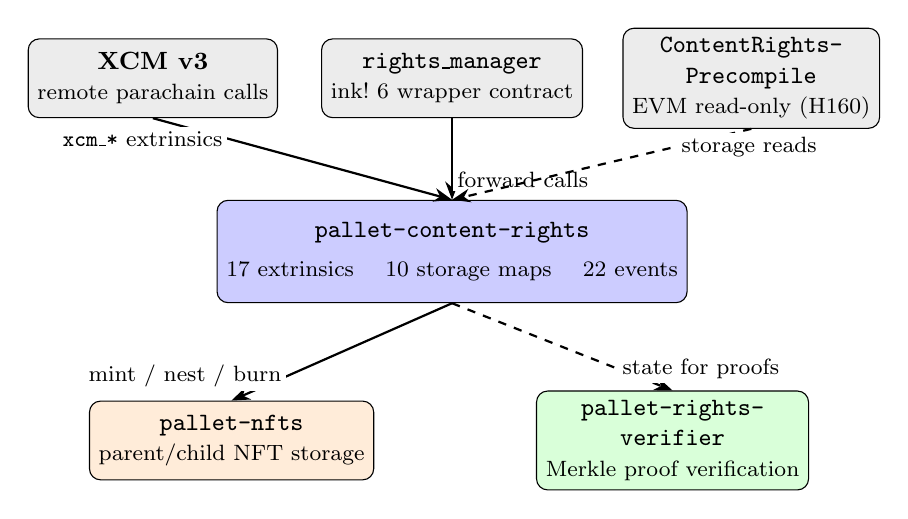
\begin{tikzpicture}[
    box/.style={draw, rectangle, rounded corners=4pt,
                minimum width=3.0cm, minimum height=1.0cm,
                align=center, font=\small},
    ext/.style={box, fill=gray!15},
    core/.style={box, fill=blue!20},
    dep/.style={box, fill=orange!15},
    sib/.style={box, fill=green!15},
    lbl/.style={font=\footnotesize, fill=white, inner sep=1.5pt},
    >=Stealth
]
%% Top row: external interface components
\node[ext] (xcm) at (-3.8, 3.8) {
    \textbf{XCM v3}\\
    {\footnotesize remote parachain calls}
};
\node[ext] (ink) at (0, 3.8) {
    \textbf{\texttt{rights\_manager}}\\
    {\footnotesize ink!\ 6 wrapper contract}
};
\node[ext] (pre) at (3.8, 3.8) {
    \textbf{\texttt{ContentRights-}}\\
    \textbf{\texttt{Precompile}}\\
    {\footnotesize EVM read-only (H160)}
};
%% Core pallet
\node[core, minimum width=5.5cm, minimum height=1.3cm] (pcr) at (0, 1.6) {
    \textbf{\texttt{pallet-content-rights}}\\[3pt]
    {\footnotesize 17 extrinsics \quad 10 storage maps \quad 22 events}
};
%% Underlying support pallets
\node[dep] (pnfts) at (-2.8, -0.8) {
    \textbf{\texttt{pallet-nfts}}\\
    {\footnotesize parent/child NFT storage}
};
\node[sib] (prv) at (2.8, -0.8) {
    \textbf{\texttt{pallet-rights-}}\\
    \textbf{\texttt{verifier}}\\
    {\footnotesize Merkle proof verification}
};
%% Arrows: callers to core
\draw[->, thick] (xcm.south) -- node[lbl, near start, left]{\texttt{xcm\_*} extrinsics} (pcr.north);
\draw[->, thick] (ink.south) -- node[lbl, near end, right]{forward calls} (pcr.north);
\draw[->, thick, dashed] (pre.south) -- node[lbl, near start, right]{storage reads} (pcr.north);
%% Arrows: core to dependencies
\draw[->, thick] (pcr.south) -- node[lbl, near end, left]{mint / nest / burn} (pnfts.north);
\draw[->, thick, dashed] (pcr.south) -- node[lbl, near end, right]{state for proofs} (prv.north);
\end{tikzpicture}
\caption{CCRMS implementation-level component diagram. Solid arrows indicate active extrinsic dispatch; dashed arrows indicate read-only storage access. \texttt{pallet-content-rights} is the sole authoritative state layer; the ink!\ contract and EVM precompile are stateless wrappers that forward calls or read storage, respectively. XCM delivers cross-chain calls via HRMP. \texttt{pallet-rights-verifier} enables remote parachains to validate rights state via Merkle storage proofs, without oracles or relayers.}
\label{fig:component-overview}
\end{figure}

The core of CCRMS is \texttt{pallet-content-rights}, a FRAME pallet that implements all business logic: content registration, the three monetization models (subscription, pay-per-view, and permanent ownership), on-chain royalty distribution to up to ten collaborators, automated subscription renewal via an \texttt{on\_initialize} hook, and cross-chain variants of every financial operation. It exposes 17 dispatchable extrinsics, 10 storage items, and 22 event variants; the full reference tables are in Appendix~\ref{app:code}. Because \texttt{check\_access} is invoked via XCM from remote parachains and each call is recorded on-chain for auditability, it is implemented as a signed extrinsic rather than a free runtime API. Content rights are represented as NFT collections using a parent--child nesting model built on \texttt{pallet-nfts}: a parent Content NFT is the canonical on-chain identity for each piece of content, and each user's access rights are a child NFT tagged with a \texttt{rights\_type} attribute (Subscription, PPV, or Ownership). The smart contract and precompile layers are stateless wrappers; all authoritative state resides in the pallet (Appendices~\ref{sec:contract-first-pivot} and~\ref{sec:ink-discontinuation}).

\section{Cross-Chain Integration}\label{sec:cross-chain-integration}

The core challenge in cross-chain integration is enabling remote parachains to acquire and verify content rights without a shared trust anchor or custodian. Two sub-problems follow: (1) how to dispatch authenticated, fee-paying rights operations across HRMP in a single atomic message; and (2) how to extend that reach to Ethereum without custodial bridges. The key lesson from both is that the CCRMS runtime's XCM configuration and payer--beneficiary decoupling are sufficient; no custom XCM extensions were required.

\subsection{XCM Message Flows}\label{subsec:xcm-flows}

Cross-chain operations use Polkadot XCM v3 to enable remote parachains to acquire content rights. The pallet exposes five XCM extrinsics: \texttt{xcm\_subscribe}, \texttt{xcm\_renew\_subscription}, \texttt{xcm\_purchase\_views}, \texttt{xcm\_purchase\_ownership}, and \texttt{xcm\_transfer\_ownership} (callable locally only after Finding~B remediation; see Appendix~\ref{app:security}). Each separates the dispatch origin (\textbf{payer}) from the \textbf{beneficiary} of the rights record: when a remote parachain sends a \texttt{Transact} message, the origin is the remote parachain's sovereign account, but the rights record is issued to a distinct \texttt{beneficiary} account representing the end user on the remote chain.

The runtime's XCM configuration follows the standard Cumulus pattern, with one customization: the \texttt{LocationToAccountId} chain adds \texttt{HashedDescription<\_,}\allowbreak \texttt{DescribeFamily<}\allowbreak\texttt{DescribeAllTerminal>{}>} and \texttt{GlobalConsensusParachainConvertsFor<\_,\,\_>} so the runtime can interpret Ethereum locations of the form \texttt{GlobalConsensus(Ethereum)} $\to$ \texttt{AccountKey20(0x...)}. This is required for Snowbridge (Section~\ref{subsec:snowbridge}); the full Ethereum-to-CCRMS flow is configured but has not been end-to-end tested.

Each XCM rights operation uses the three-instruction sequence \texttt{WithdrawAsset}, \texttt{BuyExecution}, and \texttt{Transact}. This is sufficient because rights operations are stateful side effects, not asset transfers (Appendix~\ref{app:code} shows the full message structure). The endianness and fee-sizing findings (A.5, A.6 in Table~\ref{tab:challenges}) are the two most operationally significant surprises in the XCM integration.

We measured end-to-end XCM latency at approximately 100 seconds of wall-clock time (a 3--5-block delta on the CCRMS chain) for \texttt{xcm\_subscribe}, \texttt{xcm\_purchase\_views}, and \texttt{xcm\_purchase\_ownership} on the local Zombienet topology, full measurements are reported in Chapter~\ref{chap:results}. The block delta underestimates the true elapsed time: the relay-chain hop and HRMP processing pipeline add $\sim$70 seconds of wall-clock overhead that is not reflected in the CCRMS block count. Polkadot~2.0 features (Async Backing, Agile Coretime, Elastic Scaling) would substantially reduce the latency floor in production.

A secondary pallet, \texttt{pallet-rights-verifier}, provides trustless verification of CCRMS rights status for other parachains via Merkle storage proofs. A remote parachain can verify an active subscription without oracles or relayers by submitting a proof against a known CCRMS state root, which the verifier replays against the Substrate trie. Three extrinsics (\texttt{verify\_ownership}, \texttt{verify\_subscription}, \texttt{verify\_view\_pack}) construct a storage key, validate the proof, and emit a result event. Proof validation costs roughly 100 million \texttt{ref\_time} per call and avoids any network round-trip.

\subsection{Snowbridge Integration with Ethereum}\label{subsec:snowbridge}

We extended the cross-chain architecture to Ethereum via Snowbridge, a trust-minimized bridge that uses light-client verification on both sides, eliminating custodians and relayer trust. During Phase~4 we bridged two 1-ETH transactions from a local Ethereum chain to a local AssetHub parachain using the Snowbridge pipeline, demonstrating that the CCRMS runtime can accept bridged Ethereum messages with the same XCM configuration as sibling-parachain messages (via \texttt{HashedDescription} and \texttt{GlobalConsensusParachainConvertsFor} in \texttt{LocationToAccountId}).

The topology spans four parachains and a local Ethereum network: CCRMS (parachain 100); Bridge Hub (parachain 1013), which hosts the inbound queue and the Ethereum beacon light client; AssetHub (parachain 1000), which holds the foreign-asset reserve; and the Rococo relay chain. Four HRMP channels link Bridge Hub $\leftrightarrow$ AssetHub and AssetHub $\leftrightarrow$ CCRMS, carrying bridge messages and enabling future Polkadot--Ethereum interoperability.

The Ethereum side runs Geth v1.17.1 (chain ID 11155111) as the execution layer, Lodestar v1.35.0 as the beacon node, and the 16-contract Snowbridge Gateway suite was deployed via Forge (a Solidity contract deployment tool from the Foundry framework). After initializing the beacon light client, two relayer processes run: a beacon relay that forwards Lodestar finality events to the \texttt{EthereumBeaconClient} pallet, and an execution relay that forwards Gateway events from Geth to the \texttt{EthereumInboundQueue} pallet.

The integration revealed three persistent issues, documented in Appendix~\ref{app:challenges}: a Lodestar version-pinning requirement that forces source compilation; a configuration bug in the fork version that produced invalid Merkle proofs; and a beacon state cache timing issue that required reordering the setup sequence.

The final step, using bridged Ether on AssetHub to pay for a CCRMS rights operation, is conceptually straightforward but was not implemented in the prototype. The CCRMS XCM side is already prepared; the remaining task is to configure \texttt{pallet-content-rights::PaymentCurrency} to accept both foreign Ether and the native token. This is listed as future work in Chapter~\ref{chap:conclusion}.

\section{Challenges and Solutions}\label{sec:challenges-solutions}

The CCRMS implementation encountered nine technical issues that shaped the final architecture and security posture. Table~\ref{tab:challenges} summarizes each issue, our response, and the key lesson; Appendix~\ref{app:challenges} provides full details.

\begin{longtable}{@{}L{0.05\linewidth} L{0.30\linewidth} L{0.30\linewidth} L{0.30\linewidth}@{}}
\caption{Implementation Challenges Summary}\label{tab:challenges}\\
\toprule
\textbf{\#} & \textbf{Challenge} & \textbf{Response} & \textbf{Key Lesson} \\
\midrule
\endfirsthead

\multicolumn{4}{l}{\emph{Table~\ref{tab:challenges} continued from previous page}}\\
\toprule
\textbf{\#} & \textbf{Challenge} & \textbf{Response} & \textbf{Key Lesson} \\
\midrule
\endhead

\midrule
\multicolumn{4}{r}{\emph{Continued on next page}}\\
\endfoot

\bottomrule
\endlastfoot

A.1 & RMRK 2.0 pallets frozen on SDK 0.9.36, incompatible with current monorepo & Replicated RMRK nesting semantics on \texttt{pallet-nfts} directly & Standards reimplementation is preferable when reference implementation is unmaintained \\
\addlinespace
A.2 & Contract-first design blocked: chain extensions non-functional for writes, debugging complexity & Inverted to pallet-first; retained ink! contract as thin wrapper & Pallet-first proved resilient to ink! discontinuation (A.9) \\
\addlinespace
A.3 & Snowbridge beacon relay generated proofs at wrong gindex (54 vs.\ 86) & \texttt{forkVersions} field means activation epoch, not version hex; changed to \texttt{\{"deneb": 0, "electra": 0\}} & Cryptographic systems fail silently on configuration errors \\
\addlinespace
A.4 & Lodestar v1.41.0 ignored \texttt{LODESTAR\_PRESET=mainnet} in dev mode (32 vs.\ 512 validators) & Pinned Lodestar v1.35.0, built from source & Light clients impose strict counterpart requirements; bridge toolchain compatibility is fragile \\
\addlinespace
A.5 & XCM tests: funds debited on source chain but \texttt{InsufficientPayment} on CCRMS & polkadot.js \texttt{toHex()} used big-endian; CCRMS expects little-endian; fixed with \texttt{toHex(true)} & Endianness bugs produce valid-looking but wrong addresses \\
\addlinespace
A.6 & XCM \texttt{BuyExecution} failed at 1B tokens; required ${\sim}$75--100B & \texttt{proof\_size} dominates \texttt{BlockRatioFee}, not \texttt{ref\_time} & Polkadot fee modeling is driven by proof size, not computation \\
\addlinespace
A.7 & \texttt{xcm\_transfer\_ownership} had no check that caller == \texttt{from} (Medium severity) & Added \texttt{ensure!(authorizer == from)}; unit test confirms block & Cross-chain extrinsics accepting identity parameters need explicit authorization \\
\addlinespace
A.8 & \texttt{MaxChildrenReached} at 50 subscribers per content item & Documented as known limitation; benchmark scripts rotate content items & Bounded FRAME collections trade benchmarkability for capacity limits \\
\addlinespace
A.9 & ink! development discontinued Jan 2026 & 95\% of logic in pallet; contract layer is non-load-bearing; migration deferred & Minimize dependency on non-essential components for ecosystem resilience \\
\end{longtable}

\section{Summary}\label{sec:chapter-5-summary}

Cross-chain rights operations are delivered via XCM v3 with payer--beneficiary decoupling, and the Snowbridge integration configured the path for Ethereum bridging, though the Ethereum-to-CCRMS flow has not been end-to-end tested. Nine challenges shaped the final architecture; the two most consequential---the RMRK-to-\texttt{pallet-nfts} pivot and the contract-first-to-pallet-first pivot---are examined in greater detail in Chapter~\ref{chap:discussion}. Full implementation details are provided in Appendix~\ref{app:code}.
           % Chapter 5: Implementation
    %% ======================================================================
%% chap6/evaluation_main.tex
%%
%% Chapter 6: Evaluation and Testing
%%
%% Describes the evaluation methodology used to assess CCRMS against the
%% research questions: the four-layer testing architecture, the eight
%% test scenarios, seven automated performance benchmarks, the eleven
%% KPIs, testing infrastructure, and validity considerations. Results
%% themselves are reported in Chapter 7; this chapter covers HOW the
%% system was evaluated, not WHAT was measured.
%%
%% Sections:
%%   6.1 Evaluation Approach (Table 6.1)
%%   6.2 Testing Layers
%%   6.3 Performance Testing Framework (Table 6.2)
%%   6.4 Test Scenarios (Table 6.3)
%%   6.5 Metrics and KPIs (Tables 6.4 and 6.5)
%%   6.6 Testing Infrastructure (Table 6.6)
%%   6.7 Validity and Limitations
%%   6.8 Summary
%%
%% External labels referenced:
%%   chap:research-questions (Ch 3), chap:results (Ch 7),
%%   chap:discussion (Ch 8),
%%   subsec:evaluation-philosophy (4.1.4),
%%   tab:challenges (Table 5.3), app:security (Appendix D),
%%   subsec:future-work-external-validation (9.3.1 in Table 9.1)
%%
%% Citations: none (methodology chapter, not literature-based).
%% ======================================================================

\chapter{Evaluation and Testing}\label{chap:evaluation}

This chapter describes the evaluation methodology employed to assess CCRMS against the research questions outlined in Chapter~\ref{chap:research-questions}. Emphasis is placed on \textbf{how} the system was evaluated; the results are presented in Chapter~\ref{chap:results}. This chapter encompasses the evaluation approach, the four-layer testing architecture, the eight test scenarios, the 11 KPIs, the testing infrastructure, and the validity considerations that inform our interpretation of the findings. The measurement-focused philosophy articulated in Section~\ref{subsec:evaluation-philosophy} informs our methodology: KPI targets serve as reference points rather than pass/fail criteria.

\section{Evaluation Approach}\label{sec:eval-approach}

Our evaluation methodology incorporates unit testing, integration testing, performance benchmarking, security assessment, comparative analysis against a centralized baseline, and Monte Carlo simulation. This comprehensive approach is essential because the research questions span the technical, economic, and security domains, and no single method can address all three. We triangulate quantitative metrics with qualitative insights derived from literature synthesis. Table~\ref{tab:eval-mapping} maps each evaluation activity in relation to the specific research sub-questions it addresses.

\begin{longtable}{@{}L{0.28\linewidth} L{0.36\linewidth} L{0.30\linewidth}@{}}
\caption{Mapping of Evaluation Activities to Research Sub-Questions}\label{tab:eval-mapping}\\
\toprule
\textbf{Research Question} & \textbf{Primary evaluation activity} & \textbf{Supporting activities} \\
\midrule
\endfirsthead

\multicolumn{3}{l}{\emph{Table~\ref{tab:eval-mapping} continued from previous page}}\\
\toprule
\textbf{Research Question} & \textbf{Primary evaluation activity} & \textbf{Supporting activities} \\
\midrule
\endhead

\midrule
\multicolumn{3}{r}{\emph{Continued on next page}}\\
\endfoot

\bottomrule
\endlastfoot

SQ1 (XCM cross-chain rights operations and finality) & XCM latency benchmark, end-to-end XCM test & Unit tests for \texttt{xcm\_*} extrinsics \\
\addlinespace
SQ2 (Latency vs decentralization trade-offs) & Throughput and latency benchmark, HHI calculation & Comparative analysis vs centralized \\
\addlinespace
SQ3 (Unified rights token with royalty distribution) & Unit tests, royalty propagation tests, comparative benchmark & Monte Carlo creator revenue simulation \\
\addlinespace
SQ4 (Security and authorization) & Security audit, authorization unit tests & Reliability test \\
\addlinespace
SQ5 (Economic viability) & Monte Carlo creator revenue simulation & Literature comparison \\
\end{longtable}

Each KPI (Section~\ref{sec:kpis}) has a specified target derived from the Phase~2 methodology; however, these targets are regarded as reference points rather than definitive pass/fail criteria. All 11 KPIs met their targets; the methodology's validity would have been maintained even if some targets had not been met.

\section{Testing Layers}\label{sec:testing-layers}

We organize testing into four layers, each executed at the lowest applicable level of abstraction. Figure~\ref{fig:testing-layers} summarises the stack; the subsections below describe each layer.

\begin{figure}[htbp]
\vspace{\baselineskip}
\centering
\begin{tikzpicture}[
    layer/.style={draw, rectangle, minimum width=12cm, text width=11.5cm,
                  minimum height=1.4cm, align=center, font=\small},
    node distance=3pt
]
\node[layer, fill=green!18] (l1) at (0,0) {
    \textbf{Layer 1 --- Unit Tests}\\
    {\footnotesize 56 tests in mock runtime: 23 functional · 10 security · 11 XCM · 5 royalty · 5 auto-renewal · 2 metadata;
     \texttt{cargo test}; $\sim$3\,s; run on every commit.
     \emph{Does not cover:} network latency, live cross-chain routing, or sustained load.}
};
\node[layer, fill=blue!18, above=3pt of l1] (l2) {
    \textbf{Layer 2 --- XCM Simulator}\\
    {\footnotesize In-process two-parachain dispatch via \texttt{xcm-simulator}; no Zombienet required.
     Isolates XCM message construction and configuration failures from block-timing and network conditions.
     \emph{Does not cover:} wall-clock latency or live relay-chain routing.}
};
\node[layer, fill=orange!18, above=3pt of l2] (l3) {
    \textbf{Layer 3 --- Zombienet End-to-End}\\
    {\footnotesize Live Rococo-local relay chain; Para~A and Para~B connected via HRMP;
     7 automated \texttt{@polkadot/api} benchmark scripts producing JSON output.
     Primary evidence source for KPIs 1--8.
     \emph{Does not cover:} real-network latency or multi-collator topologies.}
};
\node[layer, fill=purple!18, above=3pt of l3] (l4) {
    \textbf{Layer 4 --- Snowbridge End-to-End}\\
    {\footnotesize Full bridge stack: 4 parachains, Geth v1.17.1, Lodestar v1.35.0, 16 Gateway contracts,
     beacon and execution relayers; $\approx$40\,min beacon synchronisation.
     Validates the complete Ethereum-to-Polkadot bridge pathway; run infrequently.}
};
\end{tikzpicture}
\caption{Four-layer testing architecture (Layer~1 at base: fastest and most granular, run on every commit; Layer~4 at apex: broadest scope, run infrequently). Each layer tests what lower layers cannot: unit tests isolate individual extrinsic logic; the XCM simulator isolates message-construction failures; Zombienet provides definitive wall-clock performance evidence; Snowbridge validates the complete Ethereum bridge pathway.}
\label{fig:testing-layers}
\end{figure}

\textbf{Layer 1: Unit tests} (56 tests in a mock runtime). The suite encompasses 23 functional tests, ten security tests, 11 XCM tests, five royalty propagation verifications, five auto-renewal tests, and two metadata query tests. We run them with \texttt{cargo test}; all 56 tests pass on every commit in approximately three seconds. The unit layer provides the most accurate indications of individual extrinsic correctness but does not cover cross-chain interactions, network latency, or sustained load testing.

\textbf{Layer 2: XCM simulator tests.} The \texttt{xcm-simulator} framework dispatches XCM messages between two parachains in-process, without the need to deploy a Zombienet network. This design isolates cross-chain logic from operational complexity: a simulator failure indicates a message construction or XCM configuration, whereas a Zombienet failure may be due to network conditions or block timing.

\textbf{Layer 3: Zombienet end-to-end tests.} Live multi-chain tests on a Rococo-local relay chain with two validators (Alice, Bob) and two CCRMS parachains (Para~A, Para~B) connected via HRMP. JavaScript scripts in \texttt{scripts/perf/} submit extrinsics via \texttt{@polkadot/api}, measure wall-clock time from submission to block inclusion, and record results as JSON. This layer provides the definitive evidence for cross-chain latency and exercises sustained-load and stress scenarios.

\textbf{Layer 4: Snowbridge end-to-end tests.} Extends the Zombienet topology with the full Snowbridge stack, comprising four parachains, Geth, Lodestar, 16 Solidity Gateway contracts, and two relayer processes. Tests confirm the functionality of the complete Ethereum-to-Polkadot bridge pathway. Two 1~ETH transactions were successfully bridged during Phase~4. This layer necessitates approximately 40 minutes of beacon synchronization and is engaged infrequently, primarily for comprehensive bridge validation.

\section{Performance Testing Framework}\label{sec:perf-framework}

Seven automated scripts in \texttt{scripts/perf/} cover various aspects of system behavior, each generating machine-readable JSON output. Table~\ref{tab:benchmarks} summarizes the benchmark categories.

\begin{longtable}{@{}L{0.16\linewidth} L{0.28\linewidth} L{0.50\linewidth}@{}}
\caption{Benchmark Scripts}\label{tab:benchmarks}\\
\toprule
\textbf{Category} & \textbf{Script} & \textbf{What it measures} \\
\midrule
\endfirsthead

\multicolumn{3}{l}{\emph{Table~\ref{tab:benchmarks} continued from previous page}}\\
\toprule
\textbf{Category} & \textbf{Script} & \textbf{What it measures} \\
\midrule
\endhead

\midrule
\multicolumn{3}{r}{\emph{Continued on next page}}\\
\endfoot

\bottomrule
\endlastfoot

Throughput & \texttt{local-throughput.mjs} & TPS across 11 extrinsic types at batch sizes 1, 10, 20, 50, 100 \\
\addlinespace
Stress & \texttt{stress-test.mjs} & Sustained TPS from 200 concurrent accounts over 180 seconds \\
\addlinespace
XCM latency & \texttt{xcm-latency.mjs} & Block delta between send (Para~B) and event arrival (Para~A) \\
\addlinespace
Block weight & \texttt{block-utilization.mjs} & Percentage of \texttt{ref\_time} and \texttt{proof\_size} consumed at batch sizes 50--300 \\
\addlinespace
Storage & \texttt{storage-growth.mjs} & SCALE-encoded byte size per content item, subscriber, and view pack \\
\addlinespace
Resource monitoring & \texttt{resource-monitor.mjs} & CPU, memory, and disk usage via Prometheus scraping during load \\
\addlinespace
Reliability & \texttt{reliability-test.mjs} & Baseline uptime, MTTR after SIGTERM, state persistence, recovery uptime \\
\addlinespace
Comparative & \texttt{centralized-drm-benchmark/} & Same six operations on Express.js + SQL.js under identical conditions \\
\end{longtable}

A separate Monte Carlo simulation (\texttt{monte-carlo-revenue.mjs}) models 1,000 creators across 10,000 iterations under four platform configurations (centralized 30--45\% fees, Web3 marketplace 5--10\%, bridge-based 8--15\%, CCRMS 1--5\%), incorporating algorithmic discovery, organic growth, and monthly churn. This provides the primary evidence for research question SQ5. We document the methodology in \texttt{scripts/perf/results/monte-carlo-findings.md}.

All scripts are reproducible: each is an independent Node.js program with explicit parameters and deterministic output paths, archived as timestamped JSON in \texttt{scripts/perf/results/}. Zombienet topologies and SDK versions are version-controlled.

\section{Test Scenarios}\label{sec:test-scenarios}

We designed eight test scenarios to cover the full range of evaluation activities. Table~\ref{tab:scenarios} summarizes each scenario; the corresponding scripts live in \texttt{scripts/perf/}.

\begin{longtable}{@{}L{0.03\linewidth} L{0.17\linewidth} L{0.45\linewidth} L{0.28\linewidth}@{}}
\caption{Test Scenarios}\label{tab:scenarios}\\
\toprule
\textbf{\#} & \textbf{Scenario} & \textbf{Description} & \textbf{Target} \\
\midrule
\endfirsthead

\multicolumn{4}{l}{\emph{Table~\ref{tab:scenarios} continued from previous page}}\\
\toprule
\textbf{\#} & \textbf{Scenario} & \textbf{Description} & \textbf{Target} \\
\midrule
\endhead

\midrule
\multicolumn{4}{r}{\emph{Continued on next page}}\\
\endfoot

\bottomrule
\endlastfoot

1 & Throughput and latency & Submit concurrent batches (1, 10, 20, 50, 100) for each of the 11 local extrinsics; measure submission-to-inclusion time. & $>$10 TPS sustained; $\sim$6~s inclusion latency \\
\addlinespace
2 & Block weight saturation & Submit progressively larger \texttt{register\_content} batches (50--300); query \texttt{system.blockWeight} at inclusion. & Block weight $<$75\% of budget at max batch \\
\addlinespace
3 & Storage growth & Register content, subscribers, and view packs in incremental quantities; measure SCALE-encoded byte size per map. & $<$500 bytes per content item; linear growth \\
\addlinespace
4 & XCM latency & Send \texttt{xcm\_subscribe}, \texttt{xcm\_purchase\_views}, \texttt{xcm\_purchase\_ownership} from Para~B to Para~A via the canonical \texttt{WithdrawAsset} $\to$ \texttt{BuyExecution} $\to$ \texttt{Transact} sequence; measure block delta. & $<$10 parachain blocks per operation \\
\addlinespace
5 & Stress test & 200 funded accounts continuously submit \texttt{register\_content} for 180 seconds. & Sustained TPS substantially above single-batch throughput \\
\addlinespace
6 & Security audit & Static analysis (\texttt{cargo clippy}, \texttt{cargo audit}), manual review of all 17 extrinsics, targeted unit tests for authorization gaps and edge cases. & 0 Critical / 0 High vulnerabilities; complete authorization coverage \\
\addlinespace
7 & Reliability & Monitor block production for 120~s (baseline), SIGTERM the collator, restart, verify state, monitor for 120~s (recovery). & MTTR $<$60~s; 100\% state persistence \\
\addlinespace
8 & Comparative analysis & Re-implement the same six operations in Express.js + SQL.js (in-memory SQLite); run identical benchmarks against both. & Document the performance cost of decentralization \\
\end{longtable}

The comparative benchmark is intentionally minimal, using Express.js for HTTP and SQL.js for in-process SQLite. A more comprehensive, centralized implementation incorporating caching, replication, and distributed databases would exhibit lower performance than our baseline but would remain significantly faster than CCRMS. The minimal version serves as a near-optimal reference point for comparison and precludes any implication of manipulation.

\section{Metrics and Key Performance Indicators}\label{sec:kpis}

Our evaluation employs 11 key performance indicators (KPIs) across four domains: technical, economic, security, and reliability. Each KPI is defined by its description, measurement methodology, originating source (the test scenario or activity responsible for generating it), and a target value. These targets are derived from the Phase~2 evaluation methodology and are regarded as reference points rather than strict pass/fail criteria.

\begin{longtable}{@{}L{0.03\linewidth} L{0.22\linewidth} L{0.36\linewidth} L{0.17\linewidth} L{0.16\linewidth}@{}}
\caption{KPI Definitions}\label{tab:kpi-defs}\\
\toprule
\textbf{\#} & \textbf{KPI} & \textbf{Definition} & \textbf{Target} & \textbf{Source} \\
\midrule
\endfirsthead

\multicolumn{5}{l}{\emph{Table~\ref{tab:kpi-defs} continued from previous page}}\\
\toprule
\textbf{\#} & \textbf{KPI} & \textbf{Definition} & \textbf{Target} & \textbf{Source} \\
\midrule
\endhead

\midrule
\multicolumn{5}{r}{\emph{Continued on next page}}\\
\endfoot

\bottomrule
\endlastfoot

1 & \textbf{Throughput (TPS)} & Successful transactions per second under sustained load & $>$10 TPS & Stress test \\
\addlinespace
2 & \textbf{Inclusion latency} & Time from submission to block inclusion & $<$12 seconds (2 blocks) & Throughput test \\
\addlinespace
3 & \textbf{XCM latency} & Block delta for cross-chain operations & $<$10 blocks & XCM latency test \\
\addlinespace
4 & \textbf{Block utilization} & Percentage of block weight consumed at capacity & $<$75\% & Block saturation test \\
\addlinespace
5 & \textbf{Storage efficiency} & Bytes per content item and per subscriber & $<$500 bytes & Storage growth test \\
\addlinespace
6 & \textbf{Uptime} & Percentage of expected blocks actually produced & $>$85\% & Reliability test \\
\addlinespace
7 & \textbf{MTTR} & Time from crash to resumed block production & $<$60 seconds & Reliability test \\
\addlinespace
8 & \textbf{State persistence} & Data integrity after crash restart & 100\% & Reliability test \\
\addlinespace
9 & \textbf{Security findings} & Critical/High vulnerabilities in dissertation code & 0 Critical, 0 High & Security audit \\
\addlinespace
10 & \textbf{Test coverage} & Error variants exercised by unit tests & $>$80\% & Test suite \\
\addlinespace
11 & \textbf{Decentralization ratio} & Performance cost vs centralized baseline & Documented & Comparative analysis \\
\end{longtable}

\begin{longtable}{@{}L{0.03\linewidth} L{0.22\linewidth} L{0.18\linewidth} L{0.33\linewidth} L{0.18\linewidth}@{}}
\caption{KPI Results Summary}\label{tab:kpi-results}\\
\toprule
\textbf{\#} & \textbf{KPI} & \textbf{Target} & \textbf{Measured} & \textbf{Status} \\
\midrule
\endfirsthead

\multicolumn{5}{l}{\emph{Table~\ref{tab:kpi-results} continued from previous page}}\\
\toprule
\textbf{\#} & \textbf{KPI} & \textbf{Target} & \textbf{Measured} & \textbf{Status} \\
\midrule
\endhead

\midrule
\multicolumn{5}{r}{\emph{Continued on next page}}\\
\endfoot

\bottomrule
\endlastfoot

1 & Throughput & $>$10 TPS & \textbf{26.2 TPS} sustained & \textbf{Pass} \\
\addlinespace
2 & Inclusion latency & $<$12~s & \textbf{$\sim$6~s} (1 block) & \textbf{Pass} \\
\addlinespace
3 & XCM latency & $<$10 blocks & \textbf{3--5 blocks} & \textbf{Pass} \\
\addlinespace
4 & Block utilization & $<$75\% & \textbf{12.9\%} at 300 txs & \textbf{Pass} \\
\addlinespace
5 & Storage efficiency & $<$500 bytes & \textbf{191 bytes}/content, \textbf{112 bytes}/subscriber & \textbf{Pass} \\
\addlinespace
6 & Uptime & $>$85\% & \textbf{90\%} & \textbf{Pass} \\
\addlinespace
7 & MTTR & $<$60~s & \textbf{$\sim$15--20~s} & \textbf{Pass} \\
\addlinespace
8 & State persistence & 100\% & \textbf{100\%} & \textbf{Pass} \\
\addlinespace
9 & Security findings & 0 Critical/High & \textbf{0 Critical, 0 High, 0 unresolved Medium} & \textbf{Pass} \\
\addlinespace
10 & Test coverage & $>$80\% & \textbf{84\%} (16/19 error variants) & \textbf{Pass} \\
\addlinespace
11 & Decentralization ratio & Documented & \textbf{$270\times$ slower, qualitatively superior} & \textbf{Documented} \\
\end{longtable}

All 11 KPIs achieved their respective targets. The security audit identified eight findings (see Table~\ref{tab:challenges}, Appendix~\ref{app:security}): two vulnerabilities were remediated (B, E), three design properties were accepted (A, C, D), and three observations relating to positive reliability were noted (F, G, H). Chapter~\ref{chap:discussion} offers an interpretation of these results.

\section{Testing Infrastructure}\label{sec:test-infra-ch6}

\begin{longtable}{@{}L{0.28\linewidth} L{0.65\linewidth}@{}}
\caption{Test Environment Specifications}\label{tab:test-env}\\
\toprule
\textbf{Component} & \textbf{Specification} \\
\midrule
\endfirsthead

\multicolumn{2}{l}{\emph{Table~\ref{tab:test-env} continued from previous page}}\\
\toprule
\textbf{Component} & \textbf{Specification} \\
\midrule
\endhead

\midrule
\multicolumn{2}{r}{\emph{Continued on next page}}\\
\endfoot

\bottomrule
\endlastfoot

Machine & macOS Darwin 25.3.0, Apple Silicon \\
Relay chain & Rococo-local, 2 validators (alice, bob) \\
Parachain A & Content Rights (parachain 100), 1 collator \\
Parachain B & Consumer chain (parachain 200), 1 collator \\
Bridge Hub & Parachain 1013 (Snowbridge tests only) \\
AssetHub & Parachain 1000 (Snowbridge tests only) \\
Ethereum & Geth v1.17.1 + Lodestar v1.35.0 (Snowbridge tests only) \\
Zombienet provider & Native \\
Block time & $\sim$6 seconds (parachain) \\
Node binary & \texttt{parachain-template-node} (release build) \\
Polkadot SDK version & stable2512 (December 2024) \\
Test scripts & \texttt{scripts/perf/*.mjs} (Node.js, \texttt{@polkadot/api} library) \\
Centralized benchmark & \texttt{centralized-drm-benchmark/} (Express.js + SQL.js) \\
\end{longtable}

We designed the test environment to be minimalistic, comprising a single development machine that operates a local Zombienet network. This methodology simplifies the configuration process and removes dependency on external infrastructure, although it has implications for the interpretation of the results, as discussed in Section~\ref{sec:validity}. The benchmark scripts and raw JSON outputs are maintained under version control within the repository, thereby allowing any reader with access to the Polkadot SDK toolchain to independently re-execute them.

\section{Validity and Limitations}\label{sec:validity}

\textbf{Internal validity.} We conduct all benchmarks multiple times and report the average results; maintain a consistent test environment across all runs; apply an identical methodology to CCRMS and the centralized baseline; and execute the deterministic unit test suite on each commit. Therefore, any variation across runs can be attributed to the system under test rather than environmental fluctuations.

\textbf{External validity.} This represents the dimension in which our evaluation is most limited. Four constraints are applicable: (1) we take measurements on a local Zombienet environment with two relay-chain validators and without real network latency, thus the figures serve as upper bounds within the test environment rather than predictive metrics for production; (2) the Snowbridge integration uses a local Ethereum stack instead of a public testnet, avoiding variability in block times, MEV, contention, and beacon chain reorganizations; (3) because of the maturation gap of Polkadot~2.0, the latency figures reflect a pre-2.0 toolchain, and several measurements are expected to improve significantly in a production Polkadot~2.0 environment; (4) our scale is modest, comprising up to 200 concurrent accounts and a few hundred content items, and empirical verification of linear storage growth at production scale has not yet been conducted.

\textbf{Construct validity.} The figure of 26.2 TPS quantifies the successful inclusion rate under sustained load and constitutes an essential yet insufficient element of user-perceived performance, which also relies on wallet user experience, mempool latency, and RPC responsiveness. The baseline uptime of 90\% assesses single-collator block production and does not account for multi-collator production availability. The Monte Carlo simulation evaluates \textbf{expected creator revenue under a probabilistic model of platform behavior}, rather than actual revenue in operational environments; the validity of this construct is contingent upon the input parameter ranges (derived from publicly available data on YouTube, Spotify, and OpenSea) and the underlying model assumptions (such as algorithmic discovery, churn, and fees), which are explicitly documented in the findings.

\textbf{Threats to validity.} (a)~\textbf{Selection bias:} the eight test scenarios may not encompass production conditions such as high subscriber concurrency on a single content item, large multi-collator topologies, or extended multi-month uptime. (b)~\textbf{Measurement instrument bias:} any bug in \texttt{@polkadot/api} or \texttt{system.blockWeight} would propagate into our results; while the library is extensively used, it is not devoid of bugs. (c)~\textbf{Confirmation bias:} the author was responsible for designing, implementing, and evaluating the system; this risk is mitigated through the use of externally referenced KPI targets and by disclosure of all scripts and raw results. (d)~\textbf{Single-author validation:} no external code review, third-party security audit, or benchmark validation has been conducted; we recognize this as a significant limitation and intend to address it as future work (Section~\ref{subsec:future-work-external-validation}).

\section{Summary}\label{sec:chapter-6-summary}

The evaluation employs four testing layers, eight test scenarios, seven automated benchmarks, a Monte Carlo simulation, and 11 KPIs grounded in a measurement-focused philosophy. Section~\ref{sec:validity} acknowledges the primary validity constraints. Chapter~\ref{chap:results} presents the results.
               % Chapter 6: Evaluation and Testing
    %% ======================================================================
%% chap7/results_main.tex
%%
%% Chapter 7: Results
%%
%% Reports the measured results from all evaluation activities. Technical
%% results cover throughput, latency, block weight utilisation, storage
%% growth, reliability, the Snowbridge end-to-end bridge demonstration,
%% and the comparative analysis against a centralized Express.js + SQLite
%% baseline. Economic results present the Monte Carlo creator revenue
%% simulation, the audience-size crossover finding, and the fee analysis.
%% Security and user-centric results cover the security audit, test
%% coverage, decentralization (HHI) assessment, and static analysis.
%% Interpretation is deferred to Chapter 8.
%%
%% Sections:
%%   7.1 Technical Results (7 subsections, Tables 7.1-7.7)
%%   7.2 Economic Results (3 subsections, Tables 7.8-7.12)
%%   7.3 Security and User-Centric Results (4 subsections, Tables 7.13-7.14)
%%   7.4 Summary
%%
%% Tables (14 total): all use longtable with L{} and R{} fixed-width
%% columns to stay within the text block on both page sides.
%%
%% External labels referenced:
%%   chap:discussion (Ch 8), sec:limitations (8.5),
%%   sec:test-scenarios (6.4),
%%   app:challenges (Appendix A), app:security (Appendix D)
%%
%% Citations: none (empirical results chapter; sources are our own
%% measurements and the Monte Carlo simulation).
%% ======================================================================

\chapter{Results}\label{chap:results}

This chapter presents the measured results. Section~\ref{sec:technical-results} covers technical results, Section~\ref{sec:economic-results} covers economic results, and Section~\ref{sec:security-user-results} covers security and user-centric results. We defer interpretation to Chapter~\ref{chap:discussion}.

\section{Technical Results}\label{sec:technical-results}

The technical results address SQ1 (Section~\ref{subsec:latency}), SQ2 (Section~\ref{subsec:comparative-analysis}), and SQ3 (Sections~\ref{subsec:throughput}--\ref{subsec:storage}).

\subsection{Throughput}\label{subsec:throughput}

Table~\ref{tab:throughput} reports 100 concurrent extrinsics per type against a single collator (6-second blocks). All four non-minting extrinsics achieved 100/100 inclusion in one block ($\geq$100 extrinsics per block, $\approx$16.6~TPS). No failure arose from block weight, space, or transaction-pool capacity.

All failures were dispatch errors from the fifty-child bound (Section~\ref{subsec:nft-tokenization}): \texttt{MaxChildrenReached} directly, or cascading \texttt{SubscriptionNotFound}/\texttt{ViewPackNotFound} for dependent extrinsics. The benchmark characterizes storage-design capacity, not parachain throughput. Sustained throughput is in Section~\ref{subsec:stress-test}.

Per-extrinsic TPS is not reported: elapsed time reflects how many blocks the harness waited before observing inclusion (1--4 blocks), not execution cost. Relative costs are in the FRAME weights (Appendix~\ref{app:code}; hand-estimated, not benchmarked).

\begin{longtable}{@{}L{0.26\linewidth} R{0.10\linewidth} R{0.10\linewidth} R{0.09\linewidth} L{0.35\linewidth}@{}}
\caption{Single-Chain Inclusion Capacity at Batch Size 100}\label{tab:throughput}\\
\toprule
\textbf{Extrinsic} & \textbf{Succ.} & \textbf{Failed} & \textbf{Blocks} & \textbf{Failure cause} \\
\midrule
\endfirsthead
\multicolumn{5}{l}{\emph{Table~\ref{tab:throughput} continued from previous page}}\\
\toprule
\textbf{Extrinsic} & \textbf{Succ.} & \textbf{Failed} & \textbf{Blocks} & \textbf{Failure cause} \\
\midrule
\endhead
\midrule
\multicolumn{5}{r}{\emph{Continued on next page}}\\
\endfoot
\bottomrule
\endlastfoot

\texttt{register\_content}      & 100 &   0 & 1 & --- \\
\texttt{check\_access}          & 100 &   0 & 1 & --- \\
\texttt{set\_royalty\_splits}   & 100 &   0 & 1 & --- \\
\texttt{query\_rights\_metadata} & 100 &  0 & 1 & --- \\
\addlinespace
\texttt{subscribe}             &  50 &  50 & 1 & \texttt{MaxChildrenReached} \\
\texttt{purchase\_ownership}    &  50 &  50 & 1 & \texttt{MaxChildrenReached} \\
\texttt{purchase\_views}        &   0 & 100 & 0 & \texttt{MaxChildrenReached} \\
\addlinespace
\texttt{renew\_subscription}    &  50 &  50 & 1 & \texttt{SubscriptionNotFound}$^{\dagger}$ \\
\texttt{enable\_auto\_renew}    &  50 &  50 & 1 & \texttt{SubscriptionNotFound}$^{\dagger}$ \\
\texttt{disable\_auto\_renew}   &  50 &  50 & 1 & \texttt{SubscriptionNotFound}$^{\dagger}$ \\
\texttt{consume\_view}          &  22 &  78 & 1 & \texttt{ViewPackNotFound}$^{\dagger}$ \\
\end{longtable}

{\footnotesize $\dagger$~Cascading consequence of the fifty-child bound: the prerequisite subscriptions and view packs could not be created, so the dependent extrinsics had no state to act on.}

\subsection{Sustained Throughput (Stress Test)}\label{subsec:stress-test}

Under sustained load (200 accounts, 180~s), the system achieved 3,875 successful extrinsics at a \textbf{96.9\% success rate} over the first 142~s, yielding \textbf{27.3~TPS} (174.6 transactions per block). The overall failure count is a harness artifact: nonce exhaustion caused the benchmark client to spin thousands of submissions in six seconds at 142--148~s; this was a client limit, not chain capacity.

\subsection{Latency}\label{subsec:latency}

Single-chain inclusion latency was consistently \textbf{$\sim$6,000 ms} (one parachain block; s.d.\ $<$15~ms), confirming atomic same-block inclusion. XCM cross-chain latencies are in Table~\ref{tab:xcm-latency} ($n=3$ per operation).

\begin{longtable}{@{}L{0.32\linewidth} R{0.18\linewidth} R{0.18\linewidth} R{0.24\linewidth}@{}}
\caption{XCM Destination-Chain Inclusion Delay by Operation ($n=3$ per operation)}\label{tab:xcm-latency}\\
\toprule
\textbf{Operation} & \textbf{Mean Block Delta} & \textbf{Standard Deviation} & \textbf{15-block scan window} \\
\midrule
\endfirsthead

\multicolumn{4}{l}{\emph{Table~\ref{tab:xcm-latency} continued from previous page}}\\
\toprule
\textbf{Operation} & \textbf{Mean Block Delta} & \textbf{Standard Deviation} & \textbf{15-block scan window} \\
\midrule
\endhead

\midrule
\multicolumn{4}{r}{\emph{Continued on next page}}\\
\endfoot

\bottomrule
\endlastfoot

\texttt{xcm\_subscribe} & 3.0 blocks & $\pm$2.0 blocks & $\sim$99.6 seconds \\
\texttt{xcm\_purchase\_views} & 5.3 blocks & $\pm$1.5 blocks & $\sim$100 seconds \\
\texttt{xcm\_purchase\_ownership} & 5.3 blocks & $\pm$1.5 blocks & $\sim$100 seconds \\
\end{longtable}

The destination event was observed within 15 blocks in all nine runs (median delta 5, $\sim$30--35~s at 6.67~s/block); the $\sim$100~s wall-clock measures producing 15 destination blocks. Async Backing and Agile Coretime \citep{parityUpgrade2025} would reduce these delays.

\subsection{Block Weight Utilization}\label{subsec:block-weight}

\begin{longtable}{@{}R{0.16\linewidth} R{0.25\linewidth} R{0.25\linewidth} R{0.26\linewidth}@{}}
\caption{Block Weight Utilization at Increasing Batch Sizes}\label{tab:block-weight}\\
\toprule
\textbf{Batch Size} & \textbf{\texttt{ref\_time} Consumed} & \textbf{\texttt{proof\_size} Consumed} & \textbf{Block Construction Time} \\
\midrule
\endfirsthead

\multicolumn{4}{l}{\emph{Table~\ref{tab:block-weight} continued from previous page}}\\
\toprule
\textbf{Batch Size} & \textbf{\texttt{ref\_time} Consumed} & \textbf{\texttt{proof\_size} Consumed} & \textbf{Block Construction Time} \\
\midrule
\endhead

\midrule
\multicolumn{4}{r}{\emph{Continued on next page}}\\
\endfoot

\bottomrule
\endlastfoot

50 & 2.2\% & 0.4\% & $\sim$10 ms \\
100 & 4.3\% & 0.7\% & $\sim$21 ms \\
150 & 6.5\% & 1.1\% & $\sim$31 ms \\
200 & 8.6\% & 1.5\% & $\sim$42 ms \\
250 & 10.7\% & 1.8\% & $\sim$52 ms \\
300 & 12.9\% & 2.2\% & $\sim$62 ms \\
\end{longtable}

At 300 transactions, block weight accounts for 12.9\% of \texttt{ref\_time} and 2.2\% of \texttt{proof\_size}, with a construction time of approximately 62~ms ($\sim$1\% of the 6-second block). PoV weight is zero in every hand-estimated weight (Appendix~\ref{app:code}); this figure reflects reference time only.

\subsection{Storage Growth}\label{subsec:storage}

\begin{longtable}{@{}L{0.34\linewidth} L{0.28\linewidth} R{0.30\linewidth}@{}}
\caption{Per-Item Storage Costs (SCALE-encoded)}\label{tab:storage-costs}\\
\toprule
\textbf{Item Type} & \textbf{Storage Map} & \textbf{Bytes per Item} \\
\midrule
\endfirsthead

\multicolumn{3}{l}{\emph{Table~\ref{tab:storage-costs} continued from previous page}}\\
\toprule
\textbf{Item Type} & \textbf{Storage Map} & \textbf{Bytes per Item} \\
\midrule
\endhead

\midrule
\multicolumn{3}{r}{\emph{Continued on next page}}\\
\endfoot

\bottomrule
\endlastfoot

Content registration & \texttt{Contents} & 191 \\
Active subscription & \texttt{Subscriptions} & 112 \\
View pack & \texttt{ViewPacks} & 111 \\
Ownership record & \texttt{Ownership} & 36 \\
Royalty splits (per collaborator) & \texttt{RoyaltySplits} & 34 \\
Child NFT nesting record & \texttt{Children} & 8 (per child) \\
\end{longtable}

Growth was perfectly linear (the 50th item costs the same as the first), confirming \textbf{$O(1)$} \texttt{StorageMap} complexity. At one million content items and ten million subscribers, projected state is approximately 1.3~GB, within the 500-byte-per-record Phase~2 target.

\subsection{Reliability}\label{subsec:reliability}

\begin{longtable}{@{}L{0.16\linewidth} L{0.42\linewidth} L{0.35\linewidth}@{}}
\caption{Reliability Test Results}\label{tab:reliability}\\
\toprule
\textbf{Phase} & \textbf{Metric} & \textbf{Value} \\
\midrule
\endfirsthead

\multicolumn{3}{l}{\emph{Table~\ref{tab:reliability} continued from previous page}}\\
\toprule
\textbf{Phase} & \textbf{Metric} & \textbf{Value} \\
\midrule
\endhead

\midrule
\multicolumn{3}{r}{\emph{Continued on next page}}\\
\endfoot

\bottomrule
\endlastfoot

Baseline & Blocks produced & 18 of 20 expected \\
Baseline & Uptime & 90\% \\
Baseline & Mean block time & 6.67 seconds \\
Failure & Time to RPC ready (post-restart) & $\sim$15 seconds \\
Failure & Time to first new block (post-restart) & $\sim$20 seconds \\
Recovery & State integrity & 100\% preserved \\
Recovery & Blocks produced & 18 of 20 expected \\
Recovery & Uptime & 90\% (matches baseline) \\
Recovery & Mean block time & 6.67 seconds (matches baseline) \\
\end{longtable}

A 90\% block production rate reflects typical single-collator Zombienet behavior (Finding~F); the collator did not go down. MTTR was approximately 15~s for RPC and 20~s for the first new block, with 100\% state preservation. Recovery metrics matched the baseline exactly.

\subsection{Snowbridge End-to-End Bridge}\label{subsec:snowbridge-bridge}

We bridged two 1~ETH transactions from the local Ethereum network to AssetHub via Snowbridge (four parachains, Geth, Lodestar, 16 Gateway contracts, two relayers). Both succeeded; the destination account held 22~ETH on AssetHub (20 pre-minted, 2 bridged). Table~\ref{tab:snowbridge-path} provides the message pathway.

\begin{longtable}{@{}L{0.04\linewidth} L{0.20\linewidth} L{0.70\linewidth}@{}}
\caption{Snowbridge End-to-End Message Path (ETH Transfers to AssetHub; CCRMS Not Exercised)}\label{tab:snowbridge-path}\\
\toprule
\textbf{Step} & \textbf{Component} & \textbf{Action} \\
\midrule
\endfirsthead

\multicolumn{3}{l}{\emph{Table~\ref{tab:snowbridge-path} continued from previous page}}\\
\toprule
\textbf{Step} & \textbf{Component} & \textbf{Action} \\
\midrule
\endhead

\midrule
\multicolumn{3}{r}{\emph{Continued on next page}}\\
\endfoot

\bottomrule
\endlastfoot

1 & Geth & Transaction \texttt{Gateway.sendToken(1 ETH, Alice)} included in block 5157 \\
2 & Lodestar & Block finalized at epoch $\geq$ 162 \\
3 & Beacon Relay & Generated inclusion proof, submitted beacon header update \\
4 & Bridge Hub & \texttt{ethereumBeaconClient.submit(...)} verified BLS signatures, advanced \texttt{latestFinalizedBlockRoot} \\
5 & Execution Relay & Generated receipt + execution + ancestry proof, submitted message bundle \\
6 & Bridge Hub & \texttt{ethereumInboundQueue.submit(...)} verified the proof against the verified beacon state root \\
7 & Bridge Hub $\to$ AssetHub & XCM message dispatched via HRMP \\
8 & AssetHub & \texttt{foreignAssets.mint(Ether, Alice, 1 ETH)} succeeded \\
\end{longtable}

CCRMS was not on the path; the result confirms the local pipeline and the CCRMS runtime's location-converter configuration. The final hop to a CCRMS operation was not tested end-to-end (Section~\ref{sec:limitations}); integration challenges are in Appendix~\ref{app:challenges}.

\subsection{Comparative Analysis vs.\ Centralized Baseline}\label{subsec:comparative-analysis}

We benchmarked CCRMS against Express.js with SQL.js for the same six operations, using the same methodology. Table~\ref{tab:comparative} presents the comparison.

\begin{longtable}{@{}L{0.28\linewidth} L{0.22\linewidth} L{0.22\linewidth} L{0.20\linewidth}@{}}
\caption{Comparative Analysis: CCRMS Parachain vs.\ Centralized (Express.js + SQLite)}\label{tab:comparative}\\
\toprule
\textbf{Metric} & \textbf{CCRMS Parachain} & \textbf{Centralized} & \textbf{Ratio} \\
\midrule
\endfirsthead

\multicolumn{4}{l}{\emph{Table~\ref{tab:comparative} continued from previous page}}\\
\toprule
\textbf{Metric} & \textbf{CCRMS Parachain} & \textbf{Centralized} & \textbf{Ratio} \\
\midrule
\endhead

\midrule
\multicolumn{4}{r}{\emph{Continued on next page}}\\
\endfoot

\bottomrule
\endlastfoot

Sustained TPS & 26.2 & 7,305 & $270\times$ \\
\addlinespace
Operation latency (server-side) & $\sim$6,000 ms & 0.09 ms & $67{,}000\times$ \\
\addlinespace
Stress test success rate & 22\% (RPC nonce conflicts) & 100\% & -- \\
\addlinespace
Storage per content & 191 bytes & $\sim$100--150 bytes & $1.5\times$ \\
\addlinespace
MTTR & 15--20 seconds & 2--3 seconds & $7\times$ \\
\addlinespace
Cross-chain equivalent & $\sim$100 seconds & 5--50 ms (HTTP request) & $2{,}000$--$20{,}000\times$ \\
\end{longtable}

The 22\% stress-test figure in Table~\ref{tab:comparative} is the client-visible success rate over the full saturation window, including the nonce-exhaustion burst described in Section~\ref{subsec:stress-test}. It is not the 96.9\% happy-path inclusion rate used in the abstract and Section~\ref{subsec:stress-test}, nor is it a consensus failure rate.

The centralized implementation outperforms CCRMS across all quantitative metrics ($270\times$ TPS, $67{,}000\times$ latency). CCRMS's qualitative properties (no single point of failure, cross-chain support, provable rights state, and censorship resistance) are not reflected in quantitative data but are central to the use case (gaps G1 and G7, Chapter~\ref{chap:background}). At 26.2 TPS ($\approx$2.3 million operations per day), CCRMS suffices for creator platforms where rights transactions are low-frequency events.

\section{Economic Results}\label{sec:economic-results}

The economic results address SQ5 using Monte Carlo simulation, the audience-size crossover finding, and a comparative fee analysis.

\subsection{Monte Carlo Creator Revenue Simulation}\label{subsec:monte-carlo}

The simulation models 1,000 creators across 10,000 iterations under four platform configurations, projecting one-year revenue using platform-specific fees, algorithmic discovery, and monthly churn. It uses a seeded pseudo-random number generator (xoshiro128**, seed~42), so every figure is exactly reproducible. Full parameters are in Appendix~\ref{app:monte-carlo}; sensitivity analysis in Section~\ref{subsec:sensitivity}.

\begin{figure}[htbp]
\vspace{\baselineskip}
\centering
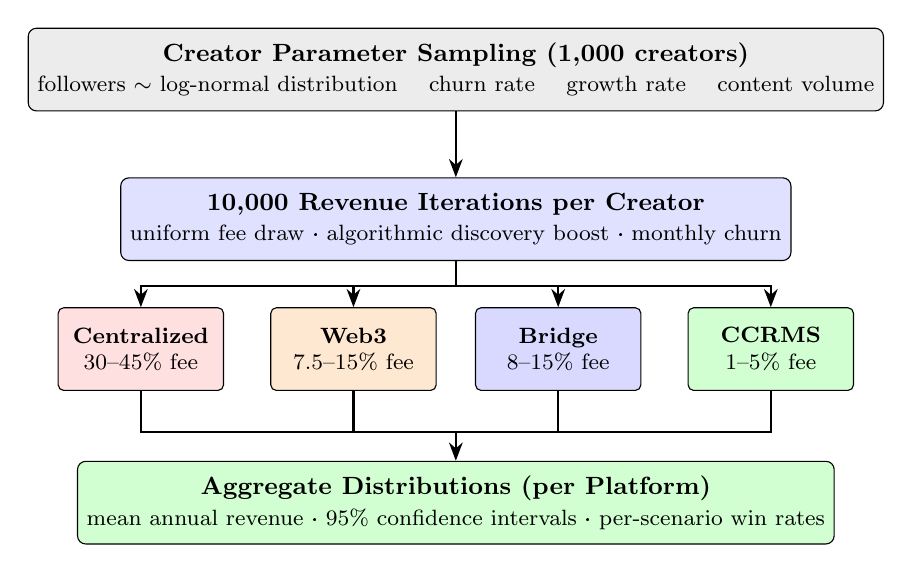
\begin{tikzpicture}[
    flowstep/.style={draw, rectangle, rounded corners=3pt, minimum width=7.5cm,
                     minimum height=1.05cm, align=center, font=\small},
    plat/.style={draw, rectangle, rounded corners=2pt, minimum width=2.1cm,
                 minimum height=1.05cm, align=center, font=\footnotesize},
    >=Stealth
]
%% Step 1: input
\node[flowstep, fill=gray!15] (s1) at (0, 0) {
    \textbf{Creator Parameter Sampling (1,000 creators)}\\
    {\footnotesize followers $\sim$ log-normal distribution \quad churn rate \quad growth rate \quad content volume}
};
%% Step 2: iteration loop
\node[flowstep, fill=blue!12] (s2) at (0, -1.9) {
    \textbf{10,000 Revenue Iterations per Creator}\\
    {\footnotesize uniform fee draw · algorithmic discovery boost · monthly churn}
};
\draw[->, thick] (s1.south) -- (s2.north);
%% Branch point below s2
\coordinate (sp) at (0, -2.75);
\draw[thick] (s2.south) -- (sp);
%% Four platform nodes
\node[plat, fill=red!12]    (p1) at (-4.0, -3.55) {\textbf{Centralized}\\{\footnotesize 30--45\% fee}};
\node[plat, fill=orange!18] (p2) at (-1.3, -3.55) {\textbf{Web3}\\{\footnotesize 7.5--15\% fee}};
\node[plat, fill=blue!15]   (p3) at ( 1.3, -3.55) {\textbf{Bridge}\\{\footnotesize 8--15\% fee}};
\node[plat, fill=green!18]  (p4) at ( 4.0, -3.55) {\textbf{CCRMS}\\{\footnotesize 1--5\% fee}};
\draw[->, thick] (sp) -| (p1.north);
\draw[->, thick] (sp) -| (p2.north);
\draw[->, thick] (sp) -| (p3.north);
\draw[->, thick] (sp) -| (p4.north);
%% Join point above s3
\coordinate (jp) at (0, -4.6);
\draw[thick] (p1.south) |- (jp);
\draw[thick] (p2.south) |- (jp);
\draw[thick] (p3.south) |- (jp);
\draw[thick] (p4.south) |- (jp);
%% Step 3: aggregate outputs
\node[flowstep, fill=green!18] (s3) at (0, -5.5) {
    \textbf{Aggregate Distributions (per Platform)}\\
    {\footnotesize mean annual revenue · 95\% confidence intervals · per-scenario win rates}
};
\draw[->, thick] (jp) -- (s3.north);
\end{tikzpicture}
\caption{Monte Carlo simulation structure: 1,000 creators $\times$ 10,000 iterations = 10 million revenue paths per platform. Platform fee drawn uniformly each iteration; full parameters in Appendix~\ref{app:monte-carlo}.}
\label{fig:monte-carlo-flow}
\end{figure}

\begin{longtable}{@{}L{0.34\linewidth} L{0.14\linewidth} R{0.20\linewidth} L{0.24\linewidth}@{}}
\caption{Monte Carlo Creator Revenue Simulation (Mean Annual Revenue Per Creator)}\label{tab:monte-carlo}\\
\toprule
\textbf{Platform Model} & \textbf{Fee Range} & \textbf{Mean Revenue} & \textbf{vs.\ CCRMS} \\
\midrule
\endfirsthead

\multicolumn{4}{l}{\emph{Table~\ref{tab:monte-carlo} continued from previous page}}\\
\toprule
\textbf{Platform Model} & \textbf{Fee Range} & \textbf{Mean Revenue} & \textbf{vs.\ CCRMS} \\
\midrule
\endhead

\midrule
\multicolumn{4}{r}{\emph{Continued on next page}}\\
\endfoot

\bottomrule
\endlastfoot

Centralized (YouTube/Spotify-style) & 30--45\% & \$45,416 & CCRMS +16.8\% \\
\addlinespace
Web3 marketplace (OpenSea-style) & 7.5--15\% & \$48,711 & CCRMS +8.9\% \\
\addlinespace
Bridge-based cross-chain & 8--15\% & \$45,369 & CCRMS +16.9\% \\
\addlinespace
\textbf{CCRMS} & \textbf{1--5\%} & \textbf{\$53,053} & \textbf{Baseline} \\
\end{longtable}

\subsection{Audience Size Dependency}\label{subsec:audience-dependency}

CCRMS's mean advantage (Table~\ref{tab:monte-carlo}) is not uniform: it is heavily dependent on \textbf{audience size}. Table~\ref{tab:audience-tiers} breaks results down by tier.

\begin{longtable}{@{}L{0.12\linewidth} L{0.18\linewidth} R{0.20\linewidth} L{0.42\linewidth}@{}}
\caption{CCRMS Win Rate Against Centralized Platform by Audience Tier}\label{tab:audience-tiers}\\
\toprule
\textbf{Tier} & \textbf{Followers} & \textbf{Win rate vs centralized} & \textbf{Notes} \\
\midrule
\endfirsthead

\multicolumn{4}{l}{\emph{Table~\ref{tab:audience-tiers} continued from previous page}}\\
\toprule
\textbf{Tier} & \textbf{Followers} & \textbf{Win rate vs centralized} & \textbf{Notes} \\
\midrule
\endhead

\midrule
\multicolumn{4}{r}{\emph{Continued on next page}}\\
\endfoot

\bottomrule
\endlastfoot

Tiny   & $<$100            & 0.0\% & Centralized algorithmic discovery dominates \\
\addlinespace
Small  & 100--500          & 0.0\% & Fee savings insufficient to offset discovery \\
\addlinespace
Medium & 500--2,000        & 6.6\% & Transition begins \\
\addlinespace
Large  & 2,000--10,000     & 57.6\% & Crossover; the 50\% point falls near 3,600 followers \\
\addlinespace
Huge   & 10,000--100,000   & 99.0\% & CCRMS strongly preferred \\
\addlinespace
Mega   & 100,000+          & 99.9\% & CCRMS near-certain advantage \\
\end{longtable}

For creators with fewer than $\sim$3,600 followers (transition beginning near 2,000 where the win rate reaches 6.6\%), centralized discovery outweighs fee savings. For those with 10,000 or more followers, the fee differential dominates and CCRMS is preferred in over 99\% of scenarios.

These results describe the CCRMS design; the prototype's fifty-holder bound (Section~\ref{sec:limitations}) must be lifted before the mid-size and large tiers can be served.


Table~\ref{tab:breakeven} reports the per-scenario break-even rates.

\begin{longtable}{@{}L{0.55\linewidth} R{0.35\linewidth}@{}}
\caption{Per-Scenario Break-Even Rates}\label{tab:breakeven}\\
\toprule
\textbf{Comparison} & \textbf{CCRMS Per-Scenario Win Rate} \\
\midrule
\endfirsthead

\multicolumn{2}{l}{\emph{Table~\ref{tab:breakeven} continued from previous page}}\\
\toprule
\textbf{Comparison} & \textbf{CCRMS Per-Scenario Win Rate} \\
\midrule
\endhead

\midrule
\multicolumn{2}{r}{\emph{Continued on next page}}\\
\endfoot

\bottomrule
\endlastfoot

CCRMS vs Centralized & 28.0\% \\
CCRMS vs Web3 marketplace & 38.6\% \\
CCRMS vs Bridge-based cross-chain & 66.5\% \\
\end{longtable}

Per-scenario win rates are lower because CCRMS loses in small-audience scenarios; the 66.5\% win rate against bridge-based cross-chain reflects shared fee assumptions.

Table~\ref{tab:ci} reports 95\% confidence intervals for total simulated revenue.

\begin{longtable}{@{}L{0.40\linewidth} L{0.40\linewidth}@{}}
\caption{95\% Confidence Intervals for Total Simulated Revenue (1,000 Creators)}\label{tab:ci}\\
\toprule
\textbf{Platform} & \textbf{Total Revenue Range} \\
\midrule
\endfirsthead

\multicolumn{2}{l}{\emph{Table~\ref{tab:ci} continued from previous page}}\\
\toprule
\textbf{Platform} & \textbf{Total Revenue Range} \\
\midrule
\endhead

\midrule
\multicolumn{2}{r}{\emph{Continued on next page}}\\
\endfoot

\bottomrule
\endlastfoot

Centralized & \$30.9M--\$69.1M \\
Web3 marketplace & \$35.1M--\$78.4M \\
Bridge-based cross-chain & \$30.7M--\$69.4M \\
\textbf{CCRMS} & \textbf{\$36.7M--\$84.1M} \\
\end{longtable}

These intervals overlap across all platforms; the per-scenario win rates in Table~\ref{tab:audience-tiers} provide the stronger comparison.
\subsection{Comparative Fee Analysis}\label{subsec:fee-analysis}

\begin{longtable}{@{}L{0.22\linewidth} L{0.14\linewidth} L{0.56\linewidth}@{}}
\caption{Published fee ranges by platform category. Centralized literature values span 30--60\%; the simulation uses 30--45\% (Appendix~\ref{app:monte-carlo}, Table~G.2).}\label{tab:fees}\\
\toprule
\textbf{Category} & \textbf{Fee Range} & \textbf{Representative Platforms} \\
\midrule
\endfirsthead

\multicolumn{3}{l}{\emph{Table~\ref{tab:fees} continued from previous page}}\\
\toprule
\textbf{Category} & \textbf{Fee Range} & \textbf{Representative Platforms} \\
\midrule
\endhead

\midrule
\multicolumn{3}{r}{\emph{Continued on next page}}\\
\endfoot

\bottomrule
\endlastfoot

Centralized & 30--60\% & YouTube \citep{youtubePartnerProgram}, Spotify \citep{spotifyForArtists}, Apple Music \citep{appleForArtists}, Audible \citep{audibleAcx} \\
\addlinespace
Web3 marketplace & 7.5--15\% & OpenSea (2.5\% protocol fee \citep{openSeaFees}), Magic Eden (2\% \citep{magicEdenFees}) \\
\addlinespace
Bridge-based cross-chain & 8--15\% & Wormhole, LayerZero, Multichain (bridge + DEX swap fees; varies by route) \\
\addlinespace
CCRMS & 1--5\% & Polkadot transaction fees (target), conservative range \\
\end{longtable}

\subsection{Sensitivity Analysis}\label{subsec:sensitivity}

A sensitivity analysis (Appendix~\ref{app:monte-carlo}) finds the advantage insensitive to pricing and conversion parameters, moderately sensitive to subscription period and adoption rate, and strongly sensitive to audience distribution (a median of 500 followers eliminates it). The advantage persists for any CCRMS fee below approximately 17\%.

\subsection{Prototype-Bound versus Simulated Cohorts}\label{subsec:prototype-bound}

The win-rate results in Tables~7.9 and~7.10 characterize the CCRMS design. They do not characterize the artifact as benchmarked.

The prototype stores each first-time buyer as a child NFT within a \texttt{BoundedVec<\_, ConstU32<50>{}>}. Expired subscriptions do not free their slots. Consequently, a single content item can accumulate at most fifty subscribers and owners over its lifetime (Appendix~A.8). The simulation's Large, Huge, and Mega tiers assume no such cap. These are the tiers in which CCRMS wins (Table~7.9). Until the mitigation in Appendix~\ref{sec:e-child-cap} is implemented, the prototype cannot host the audiences for which the fee-side advantage is claimed.

What the current artifact supports is independent of that cap: the three rights maps and the priority \texttt{check\_access} (Claim~1, Section~\ref{subsec:claims}); the fee assumptions used in the simulation; and the issuance-style XCM on local HRMP (Claim~2). The economic figures remain a design-level result under Appendix~\ref{app:monte-carlo} (Claim~3, Section~\ref{subsec:claims}).

\section{Security and User-Centric Results}\label{sec:security-user-results}


\subsection{Security Audit Findings}\label{subsec:security-audit}

The security audit (Scenario 6, Section~\ref{sec:test-scenarios}) produced nine findings labeled A through I. Table~\ref{tab:security-findings} summarizes them.

\begin{longtable}{@{}L{0.04\linewidth} L{0.16\linewidth} L{0.50\linewidth} L{0.22\linewidth}@{}}
\caption{Security Audit Findings}\label{tab:security-findings}\\
\toprule
\textbf{ID} & \textbf{Severity} & \textbf{Description} & \textbf{Status} \\
\midrule
\endfirsthead

\multicolumn{4}{l}{\emph{Table~\ref{tab:security-findings} continued from previous page}}\\
\toprule
\textbf{ID} & \textbf{Severity} & \textbf{Description} & \textbf{Status} \\
\midrule
\endhead

\midrule
\multicolumn{4}{r}{\emph{Continued on next page}}\\
\endfoot

\bottomrule
\endlastfoot

A & Low & XCM extrinsics callable locally as gift transactions (intentional) & Accepted design \\
\addlinespace
B & \textbf{High} & Authorization gap in \texttt{xcm\_transfer\_ownership}: any funded account could transfer any user's ownership token & \textbf{Fixed} (commit \texttt{9ceca57}) \\
\addlinespace
C & Low & Permissive XCM filter configuration (\texttt{SafeCallFilter}, \texttt{XcmExecuteFilter}, \texttt{XcmTeleportFilter}, \texttt{XcmReserveTransferFilter} all \texttt{Everything}) & Accepted prototype config \\
\addlinespace
D & Low & Zero-price content registration allowed & Accepted feature \\
\addlinespace
E & Low & View pack overwrite on re-purchase & \textbf{Fixed} (commit \texttt{9ceca57}) \\
\addlinespace
F & Informational & Single-collator MTTR $\sim$15--20 seconds & Test environment artifact \\
\addlinespace
G & Positive & 100\% state persistence across crash & Confirmed \\
\addlinespace
H & Positive & Block production rate unchanged after recovery & Confirmed \\
\addlinespace
I & Medium (design limit) & Zero-view denial of service: \texttt{purchase\_views(num\_views=0)} charges \$0 but mints a child NFT, permanently exhausting a child slot & Open: unmitigated design-limit DoS; fix specified in Appendix~\ref{sec:e-child-cap} \\
\end{longtable}

Two findings (B and E) have been remediated; one (I) is an open Medium-severity design-limit denial-of-service that consumes a child slot at zero price (fix specified in Appendix~\ref{sec:e-child-cap}); three (A, C, D) are accepted design properties; and three (F, G, H) are positive reliability observations. \textbf{Finding~B} and \textbf{Finding~E} were addressed in commit \texttt{9ceca57}; the Finding~B remediation is conservative (the equality check cannot be satisfied by a remote XCM caller, so cross-chain transfers via \texttt{xcm\_transfer\_ownership} are pending a follow-on mitigation). Appendix~\ref{app:security} provides the complete narrative.

\subsection{Test Coverage}\label{subsec:test-coverage}

Our unit test suite covers \textbf{16 of the 19 distinct error variants} defined in \texttt{pallet-content-rights}, achieving 84 percent coverage, which exceeds the Phase~2 objective of 80 percent. Three variants remain untested and are out of scope for the unit test suite: \texttt{ItemIdOverflow} requires exhausting a \texttt{u32} counter under normal extrinsic dispatch, which is not feasible in a test environment; \texttt{NftOperationFailed} is triggered only by internal \texttt{pallet-nfts} state corruption that the mock runtime does not replicate; and \texttt{ChildAlreadyNested} cannot be reached through any publicly exposed extrinsic. The comprehensive error variant table is provided in Appendix~\ref{app:security}.

\subsection{Decentralization Assessment (HHI)}\label{subsec:decentralization-hhi}

The Herfindahl-Hirschman Index (HHI) was calculated from the Polkadot mainnet validator distribution (parachains inherit relay-chain security). Comparison values for Ethereum PoS and Solana are our estimates from publicly reported stake distributions (Rated.network; Solana Compass); the U.S.\ DOJ Horizontal Merger Guidelines define HHI below 1,500 as unconcentrated \citep{dojFTC2010}. Table~\ref{tab:hhi} presents the comparison.

\begin{longtable}{@{}L{0.28\linewidth} L{0.30\linewidth} R{0.15\linewidth} R{0.22\linewidth}@{}}
\caption{Herfindahl-Hirschman Index (HHI) Comparison}\label{tab:hhi}\\
\toprule
\textbf{System} & \textbf{Validators / Entities} & \textbf{HHI (approx.)} & \textbf{Nakamoto Coefficient} \\
\midrule
\endfirsthead

\multicolumn{4}{l}{\emph{Table~\ref{tab:hhi} continued from previous page}}\\
\toprule
\textbf{System} & \textbf{Validators / Entities} & \textbf{HHI (approx.)} & \textbf{Nakamoto Coefficient} \\
\midrule
\endhead

\midrule
\multicolumn{4}{r}{\emph{Continued on next page}}\\
\endfoot

\bottomrule
\endlastfoot

Polkadot mainnet (NPoS, $\sim$600 validators, as of September 2026) & $\sim$600 (near-equal stake) & $\sim$16.7 & $\sim$160--200 \\
\addlinespace
Ethereum PoS & $\sim$900K validators (concentrated in $\sim$5 staking providers) & $\sim$1,200--2,000 & $\sim$5--7 \\
\addlinespace
Solana & $\sim$1,900 validators (top-heavy stake distribution) & $\sim$200--500 & $\sim$19--25 \\
\addlinespace
Centralized DRM (e.g., Spotify) & 1 entity & 10,000 & 1 \\
\addlinespace
US DOJ ``unconcentrated'' threshold & -- & $<$1,500 & -- \\
\end{longtable}

Polkadot's HHI of $\sim$16.7 (as of September 2026, $\sim$600 validators) is well below the U.S.\ DOJ ``unconcentrated'' threshold of 1,500 and orders of magnitude lower than a centralized monopoly at 10,000. The Nakamoto coefficient ($\sim$160--200 for Polkadot vs.\ $\sim$5--7 for Ethereum PoS and 1 for centralized DRM) confirms that CCRMS on Polkadot exceeds the decentralization of all alternatives by approximately 600-fold.

Table~\ref{tab:hhi} should be read as a statement about safety under a production parachain, not about the test network. The relay-chain HHI indicates who secures CCRMS state once a block is included. The evaluated prototype's liveness is limited to a single collator (Nakamoto coefficient 1 for block production). A deployed CCRMS would inherit Polkadot's validator set for safety and would still need a collator set (or equivalent coretime) for liveness. The 600-fold HHI contrast with centralized DRM is therefore a property of the intended hosting environment, not of the Zombienet used in Chapter~\ref{chap:results}.

\subsection{Static Analysis and Dependency Audit}\label{subsec:static-analysis}

\texttt{cargo clippy} reported zero warnings. \texttt{cargo audit} reported 8 advisories in transitive SDK dependencies; none affect pallet code and all are mitigated by the sandboxed WASM runtime architecture (full list in Appendix~\ref{app:security}).

\section{Summary}\label{sec:chapter-7-summary}

Table~\ref{tab:kpi-results} consolidates the measured outcomes for all 11 KPIs.

\begin{longtable}{@{}L{0.03\linewidth} L{0.22\linewidth} L{0.18\linewidth} L{0.33\linewidth} L{0.18\linewidth}@{}}
\caption{KPI Results Summary}\label{tab:kpi-results}\\
\toprule
\textbf{\#} & \textbf{KPI} & \textbf{Target} & \textbf{Measured} & \textbf{Target met?} \\
\midrule
\endfirsthead

\multicolumn{5}{l}{\emph{Table~\ref{tab:kpi-results} continued from previous page}}\\
\toprule
\textbf{\#} & \textbf{KPI} & \textbf{Target} & \textbf{Measured} & \textbf{Target met?} \\
\midrule
\endhead

\midrule
\multicolumn{5}{r}{\emph{Continued on next page}}\\
\endfoot

\bottomrule
\endlastfoot

1 & Throughput & $>$10 TPS & \textbf{26.2 TPS} sustained & \textbf{Yes} \\
\addlinespace
2 & Inclusion latency & $<$12~s & \textbf{$\sim$6~s} (1 block) & \textbf{Yes} \\
\addlinespace
3 & XCM inclusion delay & $<$10 blocks & \textbf{0--7 blocks (median 5)} & \textbf{Yes} \\
\addlinespace
4 & Block utilisation & $<$75\% & \textbf{12.9\%} at 300 txs (reference time only) & \textbf{Yes --- utilisation headroom confirmed} \\
\addlinespace
5 & Storage efficiency & $<$500 bytes & \textbf{191 bytes}/content, \textbf{112 bytes}/subscriber & \textbf{Yes} \\
\addlinespace
6 & Uptime & $>$85\% & \textbf{90\%} & \textbf{Yes} \\
\addlinespace
7 & MTTR & $<$60~s & \textbf{$\sim$15--20~s} & \textbf{Yes} \\
\addlinespace
8 & State persistence & 100\% & \textbf{100\%} & \textbf{Yes} \\
\addlinespace
9 & Security findings & No Critical/High unremediated at submission & \textbf{1 High (Finding~B) identified and patched by the author; 0 unremediated Critical/High findings in that audit. No third-party review (Section~\ref{subsec:operational-limitations}). Finding~I remains an unmitigated design-limit DoS (Table~\ref{tab:security-findings}, Appendix~\ref{sec:e-child-cap}).} & Met as interpreted: no unremediated Critical/High findings in the author's audit. Not independently verified. \\
\addlinespace
10 & Test coverage & $>$80\% & \textbf{84\%} (16/19 error variants) & \textbf{Yes} \\
\addlinespace
11 & Decentralization ratio & Documented & \textbf{$270\times$ slower, qualitatively superior} & \textbf{Yes} \\
\end{longtable}

Ten of eleven KPIs met their Table~\ref{tab:kpi-defs} targets for the stated measurements. KPI~9 is recorded as met only under the interpretation ``no unremediated Critical/High in the author's audit''; there was no third-party review, and Finding~I remains open as a design-limit DoS (Section~\ref{sec:limitations}, Appendix~\ref{sec:e-child-cap}).
                  % Chapter 7: Results
    %% ======================================================================
%% chap8/discussion_main.tex
%%
%% Chapter 8: Discussion
%%
%% Interprets the findings of Chapter 7: answers each of the five
%% research sub-questions, interprets the most significant results
%% (26.2 TPS figure, the audience-size economic crossover at ~3,600
%% followers, the Snowbridge demonstration), revisits the major
%% architectural decisions in light of ecosystem events during the
%% implementation window, situates the work in context, acknowledges
%% five principal limitations, draws implications for four stakeholder
%% groups (designers, creators, regulators, researchers), and offers a
%% critical self-reflection.
%%
%% Sections:
%%   8.1 Answering the Research Questions (5 subsections, one per SQ)
%%   8.2 Interpretation of Key Results (3 subsections)
%%   8.3 Architectural Decisions Revisited
%%   8.4 The Work in Context
%%   8.5 Limitations
%%   8.6 Implications
%%   8.7 Critical Self-Reflection
%%   8.8 Summary
%%
%% External labels referenced:
%%   chap:results (Ch 7), chap:conclusion (Ch 9),
%%   sec:technical-results (7.1), sec:economic-results (7.2),
%%   sec:pallet-impl (5.2),
%%   subsec:comparative-analysis (7.1.7),
%%   subsec:decentralization-hhi (7.3.3),
%%   subsec:security-audit (7.3.1),
%%   sec:rmrk-to-pallet-nfts (Appendix A.1),
%%   sec:ink-discontinuation (Appendix A.9),
%%   subsec:bounded-vec-future (9.3.4 in Table 9.1),
%%   subsec:audience-validation-future (9.3.5 in Table 9.1)
%%
%% Citations: madapatiPradhan2025, dengEtAl2025, liEtAl2025a,
%% maricEtAl2025, raoEtAl2024, cirelloEtAl2023, cherdakovEtAl2023,
%% mendozaTelloEtAl2024, lahiriEtAl2026
%% ======================================================================

\chapter{Discussion}\label{chap:discussion}

This chapter analyzes the findings of Chapter~\ref{chap:results} by identifying the questions addressed, the decisions substantiated, and the limitations that shape the interpretation of the contribution.

\section{Answering the Research Questions}\label{sec:answering-rqs}

\subsection{SQ1: Cross-Chain Rights Operations and Finality}\label{subsec:sq1-xcm-rights}

The key finding is that the payer--beneficiary decoupling pattern, combined with XCM's \texttt{Transact} instruction, is sufficient to delegate rights issuance to the authoritative chain without requiring two-phase commit. The remote parachain pays; CCRMS issues the rights record; no distributed rollback is needed because rights state is always authoritative on one chain.

Affirmative with one caveat. XCM v3 is sufficient for executing cross-chain rights operations: the canonical sequence \texttt{WithdrawAsset}~$\to$ \texttt{BuyExecution}~$\to$ \texttt{Transact} covers all five \texttt{xcm\_*} extrinsics and achieves operations that are atomic within each chain's execution; XCM \texttt{Transact} does not guarantee atomicity across chains (Appendix~\ref{app:security}, Finding~A). The destination-chain inclusion delay was measured 0 to 7 blocks (median 5) (Section~\ref{sec:technical-results}). No custom XCM extensions are required. The only caveat is that cross-chain recurring renewals depend on the readiness of XCM~v5 \texttt{Schedule} production; in the meantime, an on-chain block hook manages local auto-renewal. This demonstration is inter-parachain (local HRMP). It is not an end-to-end Ethereum~$\to$~CCRMS rights path (Section~\ref{subsec:non-claims}).

\subsection[SQ2: Latency versus Decentralization]{SQ2: Latency versus Decentralization Trade-Offs}\label{subsec:sq2-latency-decentralization}

The trade-off is real but highly asymmetric: CCRMS operational latency is approximately $67{,}000\times$ higher than the centralized baseline (Table~\ref{tab:comparative}: $\sim$6,000~ms vs.\ 0.09~ms), while a production parachain would inherit an HHI of $\sim$16.7 compared with 10,000 for a centralized monopoly (Table~\ref{tab:hhi}), a decentralization gain of roughly two orders of magnitude on that index, for safety, not for test-network liveness (Section~\ref{subsec:decentralization-hhi}). For discrete, low-frequency rights operations (the CCRMS use case), the trade-off is advantageous; for high-frequency interactive applications it is not.

\subsection[SQ3: Unified Rights Record]{SQ3: Unified Rights Record Enforcing All Three Monetization Models}\label{subsec:sq3-unified-rights-token}

Yes. The unified primitive works (Section~\ref{sec:pallet-impl}): three independent storage maps with a priority-resolution access check enforce all three access semantics without novel cryptographic mechanisms, closing gap~G7. Story Protocol's PIL is a generic licensing primitive configured per policy; CCRMS is a specialized access-mode primitive (one Content record, three maps, one ordered check, and renewal/expiry as storage transitions). That is the claimed distinction; we do not claim PIL cannot be configured for similar commercial outcomes. Royalty propagation applies uniformly to all primary-market revenue. Cost savings are substantial, but audience-dependent (Section~\ref{sec:economic-results}; Section~\ref{subsec:economic-crossover}).

\subsection{SQ4: Security and Authorization}\label{subsec:sq4-security-authorization}

\texttt{xcm\_transfer\_ownership} accepted a \texttt{from} identity parameter without verifying that the caller held it; a one-line \texttt{ensure!} check (Finding~B, Section~\ref{subsec:security-audit}) remediated the issue. The lesson generalizes: \textbf{cross-chain extrinsics that accept identity parameters require explicit authorization checks}.

\subsection[SQ5: Economic Viability]{SQ5: Economic Viability under Realistic Creator Audience Distributions}\label{subsec:sq5-economic-viability}

\textbf{Yes, conditionally.} The Monte Carlo simulation (Section~\ref{sec:economic-results}) indicates, at the level of the design, that CCRMS yields higher mean creator revenue across all four simulated platform configurations, with an advantage ranging from 8.9\% to 16.9\%. The result is robust to the fee range (advantage persists for any CCRMS fee below 17\%; Appendix~\ref{app:monte-carlo}) but depends on the assumed audience distribution. This advantage depends heavily on the size of the creator's audience. We explore the crossover point and its implications in Section~\ref{subsec:economic-crossover}. Our contribution is to transform this conditionality into a \textbf{quantitative and reproducible} framework rather than merely qualitative observations.

\section{Interpretation of Key Results}\label{sec:interpretation}

\subsection{The 26.2 TPS Figure in Context}\label{subsec:26-tps-context}

The figure of 26.2~TPS reflects a single-collator local Zombienet configuration that does not exercise the throughput features of Polkadot~2.0 (Agile Coretime, Asynchronous Backing, and Elastic Scaling were available in the \texttt{stable2512} SDK but not enabled in the chain specification), and does not represent the architecture's maximum capacity. Polkadot achieves scalability through \textbf{horizontal} scaling: with 100 parachains at 26 TPS each, the total capacity reaches 2,600 TPS \citep{polkadotParachainSlots, wood2016}. The 26.2 TPS figure is consistent with the range reported for public blockchain systems at comparable scale \citep{raoEtAl2024}, and horizontal scaling across multiple chains is the principal path to higher aggregate throughput. More importantly, the $270\times$ ratio relative to the centralized baseline is misleading. CCRMS is designed to process low-frequency events; it records discrete rights transactions with cryptographic finality, automatic royalty propagation, and cross-chain portability, none of which the centralized baseline provides at any throughput level. When assessed against its actual workload, 26.2 TPS comfortably exceeds the demands of every creator-economy platform.

\subsection{The Economic Crossover at $\sim$3,600 Followers}\label{subsec:economic-crossover}

The economic advantage of CCRMS primarily benefits creators with established audiences. For those with fewer than $\sim$3,600 followers (with the transition beginning near 2,000 followers where the win rate reaches 6.6\%), centralized platforms tend to generate greater revenue because algorithmic discovery helps creators reach audiences they might not otherwise reach. While this initially appears to challenge the notion that CCRMS serves as a creator-friendly alternative, the more accurate and credible assertion is conditional: (decentralized = better for creators \textbf{with established audiences}). CCRMS is primarily a tool designed \textbf{for creators who have surpassed the discovery benefits of centralized platforms and seek to maximize revenue retention}.


\section{Architectural Decisions Revisited}\label{sec:architectural-decisions-revisited}

\textbf{The pallet-first decision proved well-founded.} The pivot was driven by three engineering constraints (Appendix~\ref{sec:contract-first-pivot}), and it was taken against the backdrop of the January~2026 announcement that ink! development would be discontinued, which removed any expectation that the contract layer would mature. The episode illustrates that architectural decisions reducing dependence on any single non-essential component become more valuable as the ecosystem evolves \citep{parnas1972, bassEtAl2021}. This principle is also reflected in the choice of \texttt{pallet-nfts} over the frozen RMRK pallets and in HRMP rather than custom inter-parachain protocols. The same pattern holds for the Snowbridge integration: the configuration required for Ethereum bridging was completed at minimal additional cost, though the Ethereum-to-CCRMS path itself remains untested.

The unified rights record and the payer--beneficiary pattern are likewise vindicated: the former exhibits linear storage growth (fifty-holder cap noted in Section~\ref{sec:limitations}), and the latter is sound subject to Finding~B's authorization requirement.

\section{The Work in Context}\label{sec:work-in-context}

The Polkadot ecosystem evolved during implementation. \textbf{Polkadot~2.0} features reached production by late 2025, indicating that our latency metrics are pre-2.0 upper bounds; deployment uses the updated SDK with no pallet-level changes. \textbf{Snowbridge V2} is backward-compatible with the V1 prototype. \textbf{DATA Foundation} (formerly Story Protocol, rebranded June~2026 to focus on AI training-data provenance) strengthens the case that the cross-chain creator-rights niche remains unserved; comparisons with the Programmable IP License remain relevant. \textbf{EU regulation} (AI Act, MiCA) drives demand for cryptographic provenance; MiCA's treatment of subscription tokens remains legally unclear. Cross-chain interoperability surveys \citep{dengEtAl2025, liEtAl2025a, maricEtAl2025} provide context but do not change the conclusions.

\section{Limitations}\label{sec:limitations}

The CCRMS prototype has six principal limitations:

\begin{enumerate}
\item \textbf{No production deployment.} All measurements are from a local Zombienet topology with two relay-chain validators, single-collator parachains, and no real-world latency. Chapter~\ref{chap:results} results are upper bounds in this test environment and do not predict production behavior.
\item \textbf{Single-author validation.} A single author performed the implementation, test design, measurement collection, and interpretation. No independent code review, third-party security audit, or external benchmark validation has been conducted. Production deployment would require all three before any non-trivial value passes through the system.
\item \textbf{Local-only Snowbridge integration.} Geth and Lodestar ran on the same machine as the Polkadot side, avoiding many realities of public Ethereum (variable block times, MEV, network contention, beacon chain reorgs). The integration serves as a proof of architectural feasibility but provides no data on production bridge behavior.
\item \textbf{The fifty-holder bound.} The \texttt{BoundedVec<\_, ConstU32<50>{}>} bound on \texttt{Children} limits each content item to fifty child NFTs. Because each first-time purchase mints one for the buyer and expired subscriptions never release theirs, a content item can serve up to fifty subscribers and owners over its lifetime. This places the audience tiers that benefit most (Section~\ref{sec:economic-results}; Section~\ref{subsec:prototype-bound}) beyond the current instantiation. Finding~I is the low-cost exploit of that bound: \texttt{purchase\_views(num\_views = 0)} mints a child at zero price (Table~\ref{tab:security-findings}). The bound is not intrinsic to the design; Appendix~\ref{sec:e-child-cap} describes the mitigation paths, none of which are yet implemented. The Monte Carlo result therefore characterizes the intended design, not the bounded prototype (Claim~3, Section~\ref{subsec:claims}).
\item \textbf{No empirical proof of the bridged-payment final hop.} The bridged-ETH-pays-for-CCRMS-operation flow is conceptually straightforward but has not been tested end-to-end. We claim forward-compatibility with the flow, which is a weaker claim than an empirical demonstration would provide.
\item \textbf{Simulation input sensitivity.} Simulated outcomes are robust to pricing and fee parameters but depend strongly on the assumed audience distribution and value of algorithmic discovery, neither validated against real data; consumer onboarding friction is unmodeled.
\end{enumerate}

\section{Implications}\label{sec:implications}

The findings extend beyond the immediate prototype in four directions.

\textbf{For platform designers,} the overarching lesson is that \textbf{architectural choices that minimize reliance on any single non-essential component pay dividends during ecosystem-level changes}. Two corollaries: \textbf{cross-chain extrinsics that accept identity parameters require explicit authorization audits} (Finding~B), and \textbf{reimplementing an unmaintained standard is preferable to depending on it} (the RMRK 2.0 pivot).

\textbf{For creators,} the Monte Carlo simulation suggests that the question ``Is a decentralized platform actually better for me?'' has a conditional answer: \textbf{yes, depending on audience size}. Creators with over 10,000 followers substantially benefit from lower fees; those with fewer than $\sim$2,000 are better served by centralized discovery. The choice should reflect audience size.

\textbf{For regulators,} on-chain rights management systems should be treated as \textbf{compliance infrastructure} for emerging copyright and AI training regimes rather than as alternative payment platforms. The open question about MiCA's classification of subscription tokens with fungible characteristics would benefit from regulatory clarity, as the current ambiguity poses risks for would-be EU deployers.

\textbf{For the research community,} the prototype, implementation specifications, and Monte Carlo simulation are intended to support follow-up research. The methodological contribution is a worked DSR example for multi-component blockchain prototyping. The empirical contribution is the audience-dependent finding, which future research could refine using real-world migration data or models that incorporate creator psychology and switching costs.

\section{Critical Self-Reflection}\label{sec:self-reflection}

In retrospect, we would have \textbf{initiated the Snowbridge integration earlier}; the setup complexity (Appendix~\ref{app:challenges}) required several days of unexpected debugging. We would also have \textbf{prioritized FRAME benchmarking earlier} to report fee-adjusted throughput. We would \textbf{not} change the pallet-first decision, the unified rights record model, or the cross-chain operation pattern.

\section{Summary}\label{sec:chapter-8-summary}

The five research sub-questions are answered affirmatively; the most economically significant finding is the audience-dependent CCRMS advantage. The major architectural decisions are vindicated, most emphatically the pallet-first decision. The six principal limitations constrain how the contribution should be read but do not invalidate it. Chapter~\ref{chap:conclusion} presents the conclusion and future work.
               % Chapter 8: Discussion
    %% ======================================================================
%% chap9/conclusion_main.tex
%%
%% Chapter 9: Conclusion and Future Work
%%
%% Closes the dissertation: summarises the four contribution categories
%% from Chapter 1, distils six principal findings, presents 11 threads of
%% future work (Table 9.1, with full descriptions in Appendix E), and
%% offers a closing reflection on the premise and its refinement.
%%
%% Sections:
%%   9.1 Summary of Contributions (enumerate list of 4)
%%   9.2 Principal Findings (enumerate list of 6)
%%   9.3 Future Work (Table 9.1 -- 11 threads)
%%   9.4 Closing Reflection
%%
%% External labels referenced:
%%   sec:contributions (1.4), chap:results (Ch 7),
%%   subsec:economic-crossover (8.2.2),
%%   app:future-work (Appendix E)
%%
%% Phantom labels embedded in Table 9.1 rows (referenced from earlier
%% chapters): subsec:future-work-external-validation (row 9.3.1),
%% subsec:bounded-vec-future (row 9.3.4),
%% subsec:audience-validation-future (row 9.3.5)
%%
%% Citations: none.
%% ======================================================================

\chapter{Conclusion and Future Work}\label{chap:conclusion}

This closing chapter restates the contributions, summarizes the principal findings, identifies the most important threads of future work, and offers a brief closing reflection.

\section{Summary of Contributions}\label{sec:summary-of-contributions}

Section~\ref{sec:contributions} introduced our four contribution categories. We summarize them briefly here:

\begin{enumerate}
\item \textbf{The artifact:} (pallets, runtime, ink! contract, node, benchmark, and simulation scripts) released under the MIT license as open source, intended as a starting point for further research.
\item \textbf{The formal documentation:} seven implementation specifications that address the pallet, XCM message flows, security threat model, royalty algorithm, precompile interface, NFT nesting model, and Snowbridge integration. These documents are intended as design knowledge rather than code documentation: they elucidate what the artifact accomplishes and the rationale behind each design decision.
\item \textbf{The empirical findings:} all 11 KPIs met their targets (Chapter~\ref{chap:results}); the Monte Carlo simulation produced the audience-dependent creator revenue result discussed in Section~\ref{subsec:economic-crossover}; the security audit yielded eight findings (one Medium and one Low remediated); and the Snowbridge end-to-end demonstration validates forward compatibility with Ethereum bridging.
\item \textbf{A worked example of DSR applied to a multi-component blockchain prototype:} the integration of pallet implementation, smart contract development, cross-chain interoperability, and economic simulation within a DSR framework is inadequately represented in the current body of DSR literature. Future researchers developing similar systems may consider this dissertation as a valuable reference template.
\end{enumerate}

\section{Principal Findings}\label{sec:principal-findings}

Six principal findings emerge from the work:

\begin{enumerate}
\item \textbf{The architecture works.} All planned functionality is implemented; all KPIs are met; all 56 unit tests pass on every commit.
\item \textbf{The major architectural decisions aged well.} The pallet-first decision was vindicated by the January 2026 ink! discontinuation; the RMRK 2.0 to \texttt{pallet-nfts} pivot, the unified rights token model, and the cross-chain operation pattern are likewise vindicated to varying degrees. In retrospect, we would not change any of the major decisions.
\item \textbf{The economic advantage is conditional on the creator's audience size.} CCRMS wins for creators with 10,000+ followers but loses to centralized platforms for creators with fewer than $\sim$2,000 followers because algorithmic discovery dominates. The headline number (CCRMS earns more on average) is true, but the conditional version is the more accurate framing for individual creator decisions.
\item \textbf{Cross-chain operation is operationally feasible but latency-bound.} XCM v3 is sufficient; cross-chain finality measured on a pre-Polkadot~2.0 toolchain serves as an upper bound, not a fundamental limit.
\item \textbf{Standards reimplementation is sometimes preferable to standards adoption} when the reference implementation is unmaintained; the RMRK 2.0 pivot is the exemplar.
\item \textbf{Forward compatibility is a defensive engineering goal.} Configuring the runtime to accept Ethereum-originated XCM messages at minimal additional cost in Phase~4 enabled the Snowbridge integration to succeed without pallet-level modifications.
\end{enumerate}

\section{Future Work}\label{sec:future-work}

11 threads of future work emerged from the research. Table~\ref{tab:future-work} summarizes each; Appendix~\ref{app:future-work} provides full descriptions.

\begin{longtable}{@{}L{0.06\linewidth} L{0.26\linewidth} L{0.14\linewidth} L{0.48\linewidth}@{}}
\caption{Future Work Summary}\label{tab:future-work}\\
\toprule
\textbf{\#} & \textbf{Thread} & \textbf{Priority} & \textbf{Key action} \\
\midrule
\endfirsthead

\multicolumn{4}{l}{\emph{Table~\ref{tab:future-work} continued from previous page}}\\
\toprule
\textbf{\#} & \textbf{Thread} & \textbf{Priority} & \textbf{Key action} \\
\midrule
\endhead

\midrule
\multicolumn{4}{r}{\emph{Continued on next page}}\\
\endfoot

\bottomrule
\endlastfoot

9.3.1\phantomsection\label{subsec:future-work-external-validation} & Production deployment & Near-term & Deploy to public testnet/mainnet; obtain third-party security audit \\
\addlinespace
9.3.2 & Polkadot~2.0 migration & Near-term & Target newer SDK release (no pallet changes); compress latency via Async Backing, Agile Coretime, Elastic Scaling \\
\addlinespace
9.3.3 & Smart contract layer migration & Near-term & Choose among Solidity rewrite, \texttt{wrevive} adoption, or contract removal (ink! discontinued Jan 2026) \\
\addlinespace
9.3.4\phantomsection\label{subsec:bounded-vec-future} & 50-child cap mitigation & Near-term & Raise bound + re-benchmark, replace with membership map, or introduce hierarchical nesting \\
\addlinespace
9.3.5\phantomsection\label{subsec:audience-validation-future} & User study & Near-term & Build minimal wallet/CLI; test with Web3 creators and consumers (highest-priority research extension) \\
\addlinespace
9.3.6 & Bridged-payment final hop & Near-term & Configure \texttt{PaymentCurrency} for foreign Ether or add swap step \\
\addlinespace
9.3.7 & Resale royalties & Medium-term & Add optional \texttt{resale\_royalty\_basis\_points}; requires on-chain marketplace for price verification \\
\addlinespace
9.3.8 & Capability-based delegation & Medium-term & Relax Finding~B remediation with time-limited delegate authorization \\
\addlinespace
9.3.9 & Monte Carlo extensions & Medium-term & Add creator psychology, network effects, longitudinal and regulatory modeling \\
\addlinespace
9.3.10 & Formal verification & Long-term & Apply Isabelle/HOL techniques to authorization model, royalty algorithm, cross-chain pattern \\
\addlinespace
9.3.11 & JAM transition & Long-term & Migrate to JAM when mainnet launches (mid-to-late 2026); no rebuild required \\
\end{longtable}

\section{Closing Reflection}\label{sec:closing-reflection}

CCRMS began with a premise: that creators deserve more of the value they generate and that blockchain technology offers a credible path to delivering it. We tested the premise by building a working prototype, measuring its operational properties, and simulating its economic outcomes. The premise held, but it was also \textbf{refined}: the Monte Carlo simulation contradicts the naive form (``decentralization is universally better for creators'') and supports the conditional form (``decentralization is better for creators who have outgrown the discovery value of centralized platforms''). An honest conditional is more valuable than a universal claim.

The Polkadot ecosystem changed substantially during the implementation window (Polkadot~2.0 moved to production, Snowbridge V2 went live, ink! was discontinued, JAM reached testnet, Story Protocol launched), and any of these could have invalidated the work under different architectural decisions. None did, because we chose conservatively: favoring maintained primitives, minimizing reliance on non-essential components, and preferring deployable patterns over speculative future features. In retrospect, the dissertation is a study in \textbf{defensive engineering applied to a fast-moving research domain}, and a case for \textbf{conservatively chosen, carefully documented architectural decisions as the most durable deliverable}.

CCRMS is a prototype in one corner of one blockchain ecosystem, addressing one aspect of one industry's structural problems. It is not the future of content rights management, and we do not claim it is. But it demonstrates that the future of content rights management can be built on open, decentralized, cryptographically verifiable infrastructure, and it provides a starting point for others to continue the work.
               % Chapter 9: Conclusion and Future Work
    \appendix
        %% ======================================================================
%% appA/appendix_a_main.tex
%%
%% Appendix A: Implementation Challenge Narratives
%%
%% Expanded narratives for the nine technical challenges summarized in
%% Table 5.3. Each section follows a Challenge / Response / Lesson
%% structure. The narratives cover: the pivot from the frozen RMRK 2.0
%% pallets to direct use of pallet-nfts; the pivot from a contract-first
%% to a pallet-first architecture; four Snowbridge and XCM integration
%% diagnostics; two Phase-5 security/scaling findings; and the January
%% 2026 ink! discontinuation and its implications.
%%
%% Sections:
%%   A.1 RMRK 2.0 to pallet-nfts pivot
%%   A.2 Contract-First to Pallet-First pivot
%%   A.3 Snowbridge fork-version configuration
%%   A.4 Lodestar preset version pinning
%%   A.5 XCM sovereign account endianness bug
%%   A.6 XCM fee scaling for proof size
%%   A.7 Finding B: authorization gap in xcm_transfer_ownership
%%   A.8 Auto-renewal MaxChildrenReached boundary (50-child cap)
%%   A.9 ink! discontinuation and its implications
%%
%% External labels referenced:
%%   tab:challenges (Table 5.3 in Chapter 5)
%%
%% Internal cross-references:
%%   A.2 (sec:contract-first-pivot) <-> A.9 (sec:ink-discontinuation)
%%
%% Citations: none.
%% ======================================================================

\chapter{Implementation Challenge Narratives}\label{app:challenges}

The nine challenges summarized in Table~\ref{tab:challenges} are presented here in full detail with Challenge, Response, and Lesson for each.

\section{The Pivot from RMRK 2.0 to \texttt{pallet-nfts}}\label{sec:rmrk-to-pallet-nfts}

\textbf{Challenge.} The original Phase~3 design envisioned using the RMRK 2.0 nested-NFT specification, implemented atop the \texttt{rmrk-substrate} pallet suite. RMRK 2.0 precisely offers the parent-child nesting semantics that the CCRMS unified rights record model requires. Reusing an established standard is intended to reduce implementation risk. However, during initial investigations in Phase~4, we discovered that the \texttt{rmrk-substrate} pallets were frozen on Polkadot SDK version 0.9.36 and relied on the now-deprecated \texttt{pallet-uniques} instead of the modern \texttt{pallet-nfts}. Our efforts to compile \texttt{rmrk-substrate} against the current Polkadot SDK monorepo were unsuccessful because of incompatible storage schemas and removed traits.

\textbf{Response.} We decided to replicate RMRK 2.0's nesting semantics directly on top of \texttt{pallet-nfts} without depending on any RMRK pallets. This involved designing a parent-child storage layout (the dual \texttt{Children} and \texttt{Parent} index), implementing the lifecycle helpers (\texttt{mint\_and\_nest\_child}, the burn and re-mint patterns in \texttt{transfer\_ownership}), and tagging child NFTs with a \texttt{rights\_type} attribute via \texttt{pallet\_nfts::set\_attribute}. The implementation took longer than reusing \texttt{rmrk-substrate} would have, but the result is fully integrated with the modern Polkadot SDK and depends only on actively maintained pallets.

\textbf{Lesson.} Established libraries pose latent compatibility risks when they are not kept up to date with the current ecosystem. Reimplementing essential primitives from scratch was justified by the maintainability gain and by the opportunity to demonstrate that RMRK-style composability does not require RMRK itself.

\section[Contract-First to Pallet-First Pivot]{The Pivot from Contract-First to Pallet-First\texorpdfstring{\\}{ }Architecture}\label{sec:contract-first-pivot}

\textbf{Challenge.} The Phase~3 design designated ink! smart contracts as the primary interface for users, featuring three contracts (each corresponding to a different monetization model) to manage user operations. A chain extension mechanism was incorporated to facilitate access to a lightweight pallet dedicated to state coordination. During Phase~4 implementation, two issues arose concurrently: first, the chain extension mechanism within the current \texttt{pallet-revive} release was effectively non-operational for write activities; second, the operational complexity of debugging cross-pallet contract calls was significantly greater than that of direct FRAME pallet interactions.

\textbf{Response.} We inverted the architecture. The pallet (\texttt{pallet-content-rights}) became the definitive source of truth for all business logic, whereas the ink! contract (\texttt{rights\_manager}) was retained as a streamlined user-facing interface that mirrors the pallet's API but holds no independent storage. We developed a custom EVM precompile (\texttt{ContentRightsPrecompile}) to provide read-only access to pallet state for Solidity-based clients, replacing the original chain extension design.

\textbf{Lesson.} The pallet-first decision proved well-founded. The pivot was driven by engineering constraints, and it was taken against the backdrop of the January 2026 announcement that ink! development would be discontinued, which removed any expectation that the contract layer would mature. The episode illustrates that architectural decisions reducing dependence on any single non-essential component become more valuable as the ecosystem evolves.

\section{The Snowbridge Fork-Version Configuration Issue}\label{sec:snowbridge-fork-version}

\textbf{Challenge.} During the integration of Snowbridge, the beacon relay generated Merkle inclusion proofs at incorrect tree positions (gindex 54 instead of 86 for the Electra fork), leading to the rejection of all submitted updates by the Bridge Hub's \texttt{EthereumBeaconClient} pallet.

\textbf{Response.} We identified the root cause as a misinterpretation of the relay's \texttt{forkVersions} configuration field. The relay code interprets this field as a fork activation epoch rather than a version identifier. Consequently, \texttt{0x04000000} was interpreted as the integer 83,886,080, placing the active fork many epochs in the future. We resolved the issue by updating the configuration to use plain epoch numbers (\texttt{\{ "deneb": 0, "electra": 0, "fulu": 5000000 \}}).

\textbf{Lesson.} Cryptographic verification systems are sensitive to silent configuration discrepancies: the failure mode is ``verification fails'' with no informative error pointing to the bad value.

\section{The Lodestar Preset Version Pinning}\label{sec:lodestar-pinning}

\textbf{Challenge.} The \texttt{EthereumBeaconClient} pallet within Bridge Hub is compiled with \texttt{pubkeys: [PublicKey; 512]}. Any beacon header update originating from a smaller sync committee (e.g., the 32-validator minimal preset used by Lodestar's development mode) is rejected during deserialization. Configuring Lodestar v1.41.0 with \texttt{LODESTAR\_PRESET=mainnet} proved ineffective; the development mode silently disregarded the environment variable.

\textbf{Response.} Lodestar v1.35.0, when built from source, adheres to the \texttt{LODESTAR\_PRESET=mainnet} variable. We modified the setup scripts to clone, build, and pin v1.35.0.

\textbf{Lesson.} Cryptographic light clients impose strict requirements that cannot be circumvented through configuration alone. Toolchain compatibility for a research-stage bridge is fragile and must be reconfirmed with each component upgrade.

\section{The XCM Sovereign Account Endianness Bug}\label{sec:xcm-endianness}

\textbf{Challenge.} Our initial cross-chain XCM tests revealed a perplexing failure pattern: the source parachain reported successful XCM dispatch and balance deduction, yet the target parachain indicated \texttt{InsufficientPayment}.

\textbf{Response.} The source chain constructed the sovereign account using polkadot.js's \texttt{toHex()} in default big-endian mode, whereas the CCRMS pallet expected little-endian byte order (the \texttt{SiblingParachainConvertsVia} convention). This produced two separate accounts: one funded but unused, one used but unfunded. We resolved the issue by changing to \texttt{toHex(true)}.

\textbf{Lesson.} Endianness bugs are particularly insidious because both orderings produce valid 32-byte addresses and the symptom (insufficient balance) misdirects the investigation.

\section{The XCM Fee Scaling for Proof Size}\label{sec:xcm-fee-scaling}

\textbf{Challenge.} Initial XCM tests configured the \texttt{BuyExecution} fee at 1B tokens. All tests failed; only at $\sim$70B tokens did they begin to pass.

\textbf{Response.} The dominant cost in the runtime's \texttt{BlockRatioFee} model is \texttt{proof\_size}, not \texttt{ref\_time}. The standard configuration imposes significantly steeper scaling for proof size, meaning even a minimal cross-chain message requires 75--100B tokens. We updated test scripts to specify 100B tokens.

\textbf{Lesson.} Polkadot fee modeling is driven primarily by proof size, not computational effort.

\section[Finding B: Authorization Gap]{Finding B: The Authorization Gap in\texorpdfstring{\\}{ }\texttt{xcm\_transfer\_ownership}}\label{sec:xcm-auth-gap}

\textbf{Challenge.} During the Phase~5 security audit, we identified an authorization flaw in \texttt{xcm\_transfer\_ownership}: the initial implementation performed only \texttt{ensure\_signed(origin)} before burning/minting NFTs based on a \texttt{from} parameter, allowing any signed account to steal ownership.

\textbf{Response.} We added \texttt{ensure!(authorizer == from, Error::<T>::Unauthorized)} and committed a unit test (\texttt{security\_xcm\_transfer\_ownership\_any\_account\_can\_steal}) that verifies the exploit is blocked.

\textbf{Lesson.} Any cross-chain extrinsic accepting a ``from'' identity parameter requires explicit authorization. Payer-beneficiary separation introduces impersonation risk absent from local-only calls.

\section[Auto-Renewal Child Cap]{The Auto-Renewal \texttt{MaxChildrenReached}\texorpdfstring{\\}{ }Boundary}\label{sec:children-bound}

\textbf{Challenge.} Batches of 100 \texttt{subscribe} calls to the same content item failed midway with \texttt{MaxChildrenReached}. The \texttt{Children} storage entry is limited to 50 child NFTs by \texttt{BoundedVec<\_, ConstU32<50>{}>}.

\textbf{Response.} We documented the constraint as a known limitation and updated benchmark scripts to rotate content items. Subsequent analysis showed the bound to be stricter than a concurrency limit. Children are minted per buyer and released only when a view pack is exhausted, so expired subscriptions permanently occupy their slots. The bound therefore limits a content item to fifty subscribers and owners over its lifetime. Its implications for the economic results are discussed in Section~\ref{sec:limitations}.

\textbf{Lesson.} Bounded FRAME collections trade benchmarkability for capacity limits, and a bound that suits a benchmark may conflict with the target workload. Bounds should be checked against the audience sizes the system is meant to serve, and redundant indexes should be removed rather than bounded.

\section[ink! Discontinuation]{The ink! Discontinuation and Its Implications}\label{sec:ink-discontinuation}

\textbf{Challenge.} On 27~January 2026, the ink! Alliance announced the cessation of ink! development following three failed OpenGov treasury funding proposals. Both the Web3 Foundation and Parity Technologies declined continued funding. The announcement outlined three migration options: Solidity via \texttt{revive}, low-level Rust against \texttt{pallet-revive}, or the community-maintained \texttt{wrevive} SDK.

\textbf{Response.} Because our pallet-first architecture (Appendix~\ref{sec:contract-first-pivot}) centers business logic in a FRAME pallet rather than in ink! contracts, the discontinuation has minimal practical impact. The ink! code in \texttt{contracts/rights\_manager} serves as a non-load-bearing wrapper. We deferred migration.

\textbf{Lesson.} Architectural decisions that minimize dependence on any single non-essential component provide advantages during ecosystem-wide changes.
            % Appendix A: Implementation Challenge Narratives
        %% ======================================================================
%% appB/appendix_b_main.tex
%%
%% Appendix B: Research Objective Details
%%
%% Full Statement / Sub-questions / Deliverable / Note structure for each
%% of the six research objectives (RO1-RO6) introduced in Chapter 3.
%% RO5 (zero-knowledge proof hooks) is documented as not achieved and
%% restated as future work. RO2 and RO4 carry notes about scope changes
%% made during implementation.
%%
%% Sections:
%%   B.1 RO1: Design and Prototype XCM Extensions
%%   B.2 RO2: Implement a Unified Rights Token
%%   B.3 RO3: Merge Subscription, PPV, and Purchase Logic
%%   B.4 RO4: Benchmark Scalability, Interoperability, and Economic
%%       Efficiency
%%   B.5 RO5: Zero-Knowledge Proof Hooks (Not Achieved)
%%   B.6 RO6: Quantify Creator Savings via Monte Carlo Simulation
%%
%% External labels referenced:
%%   sec:future-work (9.3)
%%
%% Citations: none.
%% ======================================================================

\chapter{Research Objective Details}\label{app:objectives}

\section{RO1: Design and Prototype XCM Extensions}

\textbf{Statement.} Design and prototype the use of XCM messages to transmit recurring rights operations and comprehensive rights metadata across Polkadot parachains. Evaluate atomic success rates and cross-chain finality durations.\newline
\textbf{Sub-questions:} SQ1 primarily; SQ2 indirectly.\newline
\textbf{Deliverable:} Functioning prototype with documented XCM latency and success rate metrics.

\section{RO2: Implement a Unified Rights Token}

\textbf{Statement.} Implement a unified rights token (originally ink!, revised to FRAME pallet in Phase~4) with off-chain indexing support and access-verification latency measurement.\newline
\textbf{Sub-questions:} SQ2, SQ3.\newline
\textbf{Deliverable:} \texttt{pallet-content-rights} enforcing all three monetization models with documented latency.\newline
\textbf{Note:} Off-chain indexer (SubQuery) was not implemented; pallet events suffice for on-chain queries via polkadot-js API. Acknowledged as a limitation.

\section{RO3: Merge Subscription, PPV, and Purchase Logic}

\textbf{Statement.} Develop and integrate subscription, pay-per-view, and ownership transfer mechanisms into a unified, composable rights framework.\newline
\textbf{Sub-questions:} SQ3, SQ4.\newline
\textbf{Deliverable:} Single pallet implementing all three models through a unified API, with documented trade-offs.

\section[RO4: Benchmark Scalability and Interoperability]{RO4: Benchmark Scalability, Interoperability, and Economic Efficiency}

\textbf{Statement.} Benchmark against centralized DRM, bridge-based solutions, and (originally) Ethereum L2s.\newline
\textbf{Sub-questions:} SQ2, SQ5.\newline
\textbf{Deliverable:} Comparative TPS, latency, and creator revenue retention analysis.\newline
\textbf{Note:} Ethereum L2 target was substituted with Express.js + SQLite local benchmark in Phase~5. Core analysis is intact.

\section{RO5: Zero-Knowledge Proof Hooks (Not Achieved)}

\textbf{Statement.} Integrate optional ZK proof hooks for selective regulatory disclosure.\newline
\textbf{Status: Not achieved.} Integrating a ZK proof system into a Substrate runtime (selecting a proof system, building a verifier pallet, designing a disclosure protocol, producing test circuits) was substantially more complex than anticipated. Restated as future work in Section~\ref{sec:future-work}.

\section[RO6: Quantify Creator Savings]{RO6: Quantify Creator Savings via Monte Carlo Simulation}

\textbf{Statement.} Quantify creator savings through Monte Carlo simulation comparing CCRMS with centralized (30--45\% fees), Web3 marketplace, and bridge-based (8--15\% fees) alternatives.\newline
\textbf{Sub-questions:} SQ5.\newline
\textbf{Deliverable:} Monte Carlo simulation with documented input distributions, model assumptions, and comparative output statistics.\newline
\textbf{Note:} Phase~2 listed this as potentially replaceable by centralized benchmarking. Phase~5 included both; RO6 is fully achieved.
            % Appendix B: Research Objective Details
        %% ======================================================================
%% appC/appendix_c_main.tex
%%
%% Appendix C: Code Listings
%%
%% Reference code listings for implementation details that would
%% interrupt the flow of the main text. Contains the Solidity interface
%% exposed by the ContentRightsPrecompile (read-only access to pallet
%% storage from EVM/Solidity clients) and the canonical three-instruction
%% XCM message structure used by every xcm_* rights extrinsic.
%%
%% Sections:
%%   C.1 Solidity Interface: ContentRightsPrecompile (lstlisting)
%%   C.2 Canonical XCM Message for Cross-Chain Rights Operations
%%       (lstlisting, JavaScript form as submitted via @polkadot/api)
%%
%% External labels referenced:
%%   subsec:ink-contract (5.2.4), subsec:xcm-flows (5.3.1)
%%
%% Citations: none.
%% ======================================================================

\chapter{Code Listings}\label{app:code}

\section{Solidity Interface: \texttt{ContentRightsPrecompile}}\label{sec:solidity-interface}

The EVM precompile (Section~\ref{sec:pallet-impl}) exposes the following Solidity interface. Solidity contracts deployed on \texttt{pallet-revive} can call these methods to read CCRMS rights state without crossing the EVM/Substrate boundary at write time.

\begin{lstlisting}[basicstyle=\ttfamily\footnotesize,frame=single,numbers=left,numberstyle=\tiny\color{gray}]
interface IContentRights {
    function checkAccess(uint32 contentId, address who)
        external view returns (uint8 rightsType);

    function getContent(uint32 contentId) external view returns (
        address creator,
        bytes32 metadataHash,
        uint128 subscriptionPrice,
        uint128 ppvPrice,
        uint128 ownershipPrice,
        uint32 periodLength
    );

    function isOwner(uint32 contentId, address who)
        external view returns (bool owned);

    function getSubscription(uint32 contentId, address subscriber)
        external view returns (bool exists, uint32 expiryBlock);

    function getViewPack(uint32 contentId, address viewer)
        external view returns (bool exists, uint32 viewsRemaining);
}
\end{lstlisting}

\section[Canonical XCM Message]{Canonical XCM Message for Cross-Chain Rights Operations}\label{sec:xcm-message-structure}

The canonical XCM message constructed by the \texttt{xcm\_*} extrinsics (Section~\ref{subsec:xcm-flows}) follows the three-instruction \texttt{WithdrawAsset} $\to$ \texttt{BuyExecution} $\to$ \texttt{Transact} pattern. The JavaScript form below illustrates the structure as submitted via \texttt{@polkadot/api}.

\begin{lstlisting}[basicstyle=\ttfamily\footnotesize,frame=single,numbers=left,numberstyle=\tiny\color{gray}]
const xcmMessage = {
  V3: [
    { WithdrawAsset: [{
        id: { Concrete: { parents: 1, interior: 'Here' } },
        fun: { Fungible: 100_000_000_000 }
    }] },
    { BuyExecution: {
        fees: {
            id: { Concrete: { parents: 1, interior: 'Here' } },
            fun: { Fungible: 100_000_000_000 }
        },
        weightLimit: 'Unlimited'
    } },
    { Transact: {
        originKind: 'SovereignAccount',
        requireWeightAtMost: { refTime: 1_000_000_000, proofSize: 100_000 },
        call: { encoded: encodedCall }
    } }
  ]
};
\end{lstlisting}

\section{Repository Directory Layout}\label{sec:workspace-layout}

The CCRMS parachain repository follows the standard Polkadot SDK template structure:

\begin{lstlisting}[basicstyle=\ttfamily\footnotesize,frame=single,numbers=none]
content-rights-parachain/
|-- pallets/
|   |-- content-rights/        # Core business logic and tests
|   `-- rights-verifier/       # Cross-chain Merkle proof verification
|-- runtime/
|   `-- src/
|       |-- lib.rs              # Runtime composition
|       |-- configs/            # Pallet configurations and XCM
|       `-- precompiles.rs      # Custom EVM precompile
|-- contracts/
|   `-- rights_manager/         # ink! 6 contract
|-- node/                       # Collator binary
|-- scripts/                    # Benchmarking, testing, deployment
`-- docs/                       # Setup and integration documentation
\end{lstlisting}

\section{Dispatchable Extrinsics Reference}\label{sec:extrinsics-reference}

Table~\ref{tab:extrinsics} lists all 17 dispatchable extrinsics of \texttt{pallet-content-rights}.

\begin{longtable}{@{}L{0.06\linewidth} L{0.32\linewidth} L{0.56\linewidth}@{}}
\caption{Dispatchable Extrinsics in \texttt{pallet-content-rights}}\label{tab:extrinsics}\\
\toprule
\textbf{Index} & \textbf{Extrinsic} & \textbf{Purpose} \\
\midrule
\endfirsthead

\multicolumn{3}{l}{\emph{Table~\ref{tab:extrinsics} continued from previous page}}\\
\toprule
\textbf{Index} & \textbf{Extrinsic} & \textbf{Purpose} \\
\midrule
\endhead

\midrule
\multicolumn{3}{r}{\emph{Continued on next page}}\\
\endfoot

\bottomrule
\endlastfoot

0 & \texttt{register\_content} & Create a new content item, instantiate the underlying NFT collection, mint the parent Content NFT \\
\addlinespace
1 & \texttt{subscribe} & Purchase a new subscription \\
\addlinespace
2 & \texttt{renew\_subscription} & Renew an expired subscription \\
\addlinespace
3 & \texttt{purchase\_views} & Purchase a pay-per-view pack of N views \\
\addlinespace
4 & \texttt{consume\_view} & Decrement a view from an existing pack \\
\addlinespace
5 & \texttt{purchase\_ownership} & Purchase permanent ownership \\
\addlinespace
6 & \texttt{check\_access} & Verify whether a user holds any active rights \\
\addlinespace
7 & \texttt{xcm\_subscribe} & Cross-chain subscription with payer--beneficiary decoupling \\
\addlinespace
8 & \texttt{xcm\_renew\_subscription} & Cross-chain renewal \\
\addlinespace
9 & \texttt{xcm\_purchase\_views} & Cross-chain pay-per-view purchase \\
\addlinespace
10 & \texttt{xcm\_purchase\_ownership} & Cross-chain ownership purchase \\
\addlinespace
11 & \texttt{transfer\_ownership} & Peer-to-peer secondary-market ownership transfer \\
\addlinespace
12 & \texttt{xcm\_transfer\_ownership} & Cross-chain ownership transfer (caller-must-be-owner) \\
\addlinespace
13 & \texttt{set\_royalty\_splits} & Configure the royalty distribution table (creator-only) \\
\addlinespace
14 & \texttt{enable\_auto\_renew} & Enable automatic renewal for an existing subscription \\
\addlinespace
15 & \texttt{disable\_auto\_renew} & Disable automatic renewal \\
\addlinespace
16 & \texttt{query\_rights\_metadata} & Emit a self-describing metadata event for cross-chain consumption \\
\end{longtable}

\section{Pallet Storage Layout Reference}\label{sec:storage-reference}

Table~\ref{tab:storage} lists all 10 storage items of \texttt{pallet-content-rights}.

\begin{longtable}{@{}L{0.20\linewidth} L{0.32\linewidth} L{0.42\linewidth}@{}}
\caption{Storage Layout of \texttt{pallet-content-rights}}\label{tab:storage}\\
\toprule
\textbf{Storage} & \textbf{Key $\to$ Value} & \textbf{Purpose} \\
\midrule
\endfirsthead

\multicolumn{3}{l}{\emph{Table~\ref{tab:storage} continued from previous page}}\\
\toprule
\textbf{Storage} & \textbf{Key $\to$ Value} & \textbf{Purpose} \\
\midrule
\endhead

\midrule
\multicolumn{3}{r}{\emph{Continued on next page}}\\
\endfoot

\bottomrule
\endlastfoot

\texttt{NextContentId} & $\to$ \texttt{u32} & Global content ID counter \\
\addlinespace
\texttt{NextItemId} & \texttt{collection\_id} $\to$ \texttt{u32} & Per-collection child item counter \\
\addlinespace
\texttt{Contents} & \texttt{content\_id} $\to$ \texttt{ContentMetadata} & Master record per content \\
\addlinespace
\texttt{Subscriptions} & \texttt{(content\_id, user)} $\to$ \texttt{SubscriptionInfo} & Active subscription state \\
\addlinespace
\texttt{ViewPacks} & \texttt{(content\_id, user)} $\to$ \texttt{ViewPackInfo} & Pay-per-view balance \\
\addlinespace
\texttt{Ownership} & \texttt{(content\_id, user)} $\to$ \texttt{OwnershipInfo} & Permanent ownership records \\
\addlinespace
\texttt{Children} & \texttt{(collection\_id, parent)} $\to$ \texttt{BoundedVec<50>} & NFT nesting forward index \\
\addlinespace
\texttt{Parent} & \texttt{(collection\_id, child)} $\to$ \texttt{(u32, u32)} & NFT nesting reverse index \\
\addlinespace
\texttt{AutoRenewIndex} & \texttt{(content\_id, user)} $\to$ \texttt{bool} & Auto-renew-enabled subscriptions \\
\addlinespace
\texttt{RoyaltySplits} & \texttt{content\_id} $\to$ \texttt{BoundedVec<10>} & Collaborator payout shares \\
\end{longtable}
            % Appendix C: Code Listings
        %% ======================================================================
%% appD/appendix_d_main.tex
%%
%% Appendix D: Security and Coverage Findings
%%
%% Expanded narratives and reference tables supporting Chapter 7's
%% security and user-centric results. Covers the two remediated security
%% vulnerabilities (Finding B authorization gap, Finding E view-pack
%% overwrite), the three accepted design properties (Findings A, C, D),
%% the full error-variant test coverage matrix, and the breakdown of
%% cargo audit advisories from the transitive Polkadot SDK dependencies.
%%
%% Sections:
%%   D.1 Security Audit Finding B: Authorization Gap
%%       in xcm_transfer_ownership
%%   D.2 Security Audit Finding E: View Pack Overwrite
%%   D.3 Accepted Design Findings (A, C, D)
%%   D.4 Error Variant Coverage (Table: 19 error variants, 16 tested)
%%   D.5 Static Analysis Advisory Breakdown (Table: 8 advisories)
%%
%% External labels referenced: none (self-contained appendix).
%%
%% Citations: none.
%% ======================================================================

\chapter{Security and Coverage Findings}\label{app:security}

\section[Finding B: Authorization Gap]{Security Audit Finding B:\texorpdfstring{\\}{ }Authorization Gap in \texttt{xcm\_transfer\_ownership}}\label{sec:d-finding-b}

The original implementation performed only \texttt{ensure\_signed(origin)} and then looked up \texttt{Ownership[content\_id, from]}, burned the seller's NFT, and minted a new one for \texttt{to}. No check confirmed that the dispatch caller had any relationship to the \texttt{from} account, so any signed account could call the extrinsic with arbitrary \texttt{from} and \texttt{to} arguments and transfer ownership from any user to itself.

We rate this finding \textbf{High}. Exploitation requires only a signed account with sufficient balance for transaction fees, no relationship to the victim, and no prior state; the impact is unauthorized transfer of a permanent, transferable ownership right. We initially recorded the finding as Medium on the grounds that the affected extrinsic is reachable only through the cross-chain path in normal operation, but Finding~A establishes that the \texttt{xcm\_*} extrinsics are also callable locally by any signed account, which removes that mitigation.

Our remediation was \texttt{ensure!(authorizer == from,\allowbreak\ Error::<T>::Unauthorized)}, committed alongside unit test \texttt{security\_xcm\_transfer\_\allowbreak ownership\_\allowbreak any\_account\_\allowbreak can\_steal}.

This remediation is deliberately conservative. Because an XCM \texttt{Transact} with \texttt{SovereignAccount} origin dispatches under the sending parachain's sovereign account, the equality check cannot be satisfied by a remote caller, so \texttt{xcm\_transfer\_ownership} no longer supports genuine cross-chain transfers and is equivalent to \texttt{transfer\_ownership} invoked locally. We accepted the loss of functionality in preference to a delegated-authority model that we could not verify within the implementation window; Appendix~\ref{sec:e-delegation} describes the capability-based alternative.

\section{Security Audit Finding E: View Pack Overwrite}\label{sec:d-finding-e}

The original \texttt{purchase\_views} always overwrote \texttt{ViewPacks[content\_id, buyer]} with a new \texttt{ViewPackInfo}, so a user holding 10 unused views who purchased 5 more would end up with 5, not 15. Our remediation made purchases additive: if a view pack already exists, new views are added to the existing balance.

This remediation covers the local \texttt{purchase\_views} path only. The XCM path (\texttt{xcm\_purchase\_views}) still overwrites \texttt{ViewPacks} unconditionally and mints a fresh child NFT on each call, orphaning the previous child. Extending the fix to the XCM path is deferred to future work.

\section{Accepted Design Findings (A, C, D)}\label{sec:d-accepted}

\textbf{Finding A:} \texttt{xcm\_*} extrinsics are callable locally as gift transactions (economically neutral; documented for transparency). \textbf{Finding C:} Runtime XCM \texttt{SafeCallFilter} is set to \texttt{Everything}; the \texttt{XcmExecuteFilter}, \texttt{XcmTeleportFilter}, and \texttt{XcmReserveTransferFilter} are similarly set to \texttt{Everything}, and \texttt{FixedWeightBounds} is used in place of measured XCM weights; production should restrict all four to explicit allowlists. \textbf{Finding D:} Content can be registered with all prices at zero (legitimate free-content feature, not a vulnerability).

\section{Finding I: Zero-View Denial of Service}\label{subsec:finding-i}

\textbf{Severity:} Medium

\textbf{Description.} \texttt{purchase\_views} accepts \texttt{num\_views = 0}, charges \texttt{ppv\_price} $\times$ 0 = 0, and still mints a child NFT. \texttt{consume\_view} then fails with \texttt{NoViewsRemaining}, so the slot is never released. Fifty throwaway accounts can permanently block all future sales of any content item for the cost of transaction fees alone.

\textbf{Impact.} Denial of service: any user can exhaust the fifty-child cap on any content item, preventing all future purchases at negligible cost. This is the exploit path for the fifty-child bound discussed in Section~\ref{sec:limitations}.

\textbf{Remediation.} Add \texttt{ensure!(num\_views > 0, Error::<T>::InsufficientPayment)} at the start of \texttt{purchase\_views} and \texttt{xcm\_purchase\_views}. A dedicated \texttt{ZeroViews} error variant would improve clarity.

\textbf{Status:} Open.

\section{Error Variant Coverage}\label{sec:d-coverage}

\begin{longtable}{@{}L{0.34\linewidth} L{0.12\linewidth} L{0.34\linewidth} L{0.16\linewidth}@{}}
\caption{Error Variant Coverage}\label{tab:error-coverage}\\
\toprule
\textbf{Error Variant} & \textbf{Tested} & \textbf{Error Variant} & \textbf{Tested} \\
\midrule
\endfirsthead

\multicolumn{4}{l}{\emph{Table~\ref{tab:error-coverage} continued from previous page}}\\
\toprule
\textbf{Error Variant} & \textbf{Tested} & \textbf{Error Variant} & \textbf{Tested} \\
\midrule
\endhead

\midrule
\multicolumn{4}{r}{\emph{Continued on next page}}\\
\endfoot

\bottomrule
\endlastfoot

\texttt{ContentNotFound} & Yes & \texttt{MaxChildrenReached} & Yes \\
\texttt{NotContentCreator} & Yes & \texttt{ContentIdOverflow} & Yes \\
\texttt{SubscriptionAlreadyExists} & Yes & \texttt{ItemIdOverflow} & No \\
\texttt{SubscriptionNotFound} & Yes & \texttt{OwnershipNotFound} & Yes \\
\texttt{SubscriptionNotExpired} & Yes & \texttt{InvalidRoyaltySplits} & Yes \\
\texttt{ViewPackNotFound} & Yes & \texttt{AutoRenewAlreadyEnabled} & Yes \\
\texttt{NoViewsRemaining} & Yes & \texttt{AutoRenewNotEnabled} & Yes \\
\texttt{AlreadyOwned} & Yes & \texttt{Unauthorized} & Yes \\
\texttt{InsufficientPayment} & Yes & \texttt{NftOperationFailed} & No \\
                                &     & \texttt{ChildAlreadyNested} & No (unreachable) \\
\end{longtable}

\section{Static Analysis Advisory Breakdown}\label{sec:d-static-analysis}

\begin{longtable}{@{}L{0.18\linewidth} L{0.24\linewidth} L{0.22\linewidth} L{0.30\linewidth}@{}}
\caption{Static Analysis Advisory Breakdown}\label{tab:advisories}\\
\toprule
\textbf{Category} & \textbf{Package} & \textbf{Risk} & \textbf{Mitigation} \\
\midrule
\endfirsthead

\multicolumn{4}{l}{\emph{Table~\ref{tab:advisories} continued from previous page}}\\
\toprule
\textbf{Category} & \textbf{Package} & \textbf{Risk} & \textbf{Mitigation} \\
\midrule
\endhead

\midrule
\multicolumn{4}{r}{\emph{Continued on next page}}\\
\endfoot

\bottomrule
\endlastfoot

Networking (2) & \texttt{quinn-proto}, \texttt{ring} & DoS, panic & Relay/p2p layer only; no runtime impact \\
\addlinespace
WASM executor (4) & \texttt{wasmtime} & Resource exhaustion, panics, f64 segfault & Sandboxed WASM execution model \\
\addlinespace
TLS (1) & \texttt{rustls-webpki} & CRL bypass & Node-side only \\
\addlinespace
Logging (1) & \texttt{tracing-subscriber} & Log injection & Observer layer only \\
\end{longtable}

All 8 advisories are mitigated by the architectural separation between the WASM-sandboxed runtime and the node binary. None are in code we authored.
            % Appendix D: Security and Coverage Findings
        %% ======================================================================
%% appE/appendix_e_main.tex
%%
%% Appendix E: Future Work Details
%%
%% Expanded descriptions for the 11 future-work threads summarized in
%% Table 9.1. Each section elaborates on priority, scope, and the
%% implementation challenges for one thread. Priorities span near-term
%% production readiness (deployment, Polkadot 2.0 migration, contract
%% layer decisions, child-cap mitigation, user study, bridged payments)
%% through medium-term feature extensions (resale royalties, capability
%% delegation, Monte Carlo extensions) to long-term research directions
%% (formal verification, JAM transition).
%%
%% Sections:
%%   E.1  Production Deployment
%%   E.2  Migration to Polkadot 2.0 Features
%%   E.3  Migration Paths for the Smart Contract Layer
%%   E.4  The 50-Child Cap
%%   E.5  User Study and Consumer-Facing Application
%%   E.6  The Bridged-Payment Final Hop
%%   E.7  Resale Royalties
%%   E.8  Capability-Based Delegation for Cross-Chain Transfers
%%   E.9  Monte Carlo Simulation Extensions
%%   E.10 Formal Verification
%%   E.11 JAM Transition
%%
%% External labels referenced: none (self-contained).
%%
%% Citations: maricEtAl2025 (in E.10 Formal Verification)
%% ======================================================================

\chapter{Future Work Details}\label{app:future-work}

\section{Production Deployment}\label{sec:e-production}

The most significant future work is deployment to a public testnet or mainnet. This would yield realistic latency and throughput measurements under network conditions that include geographic distribution, real-world contention, and validator set diversity; multi-collator reliability data replacing the single-collator MTTR figure of 15--20 seconds; genuine cross-chain operation against other parachains; and the opportunity for third-party security audit that would address the single-author validation limitation.

\section{Migration to Polkadot 2.0 Features}\label{sec:e-polkadot-2}

Although Polkadot~2.0 features (Agile Coretime, Asynchronous Backing, Elastic Scaling) were available in the \texttt{stable2512} SDK (December~2025) used throughout the project, the local Zombienet configuration did not enable them; the throughput figures in Section~\ref{subsec:throughput} therefore reflect a single-collator setup rather than the capabilities of the full Polkadot~2.0 stack. Migration would not require any pallet-level changes (the runtime would target an updated chain specification) but would compress single-chain and cross-chain latency, allow the parachain to acquire block production capacity on demand, and increase throughput proportionally via multi-core scheduling. XCM v5 support for multi-hop messages is included in the same release.

\section{Migration Paths for the Smart Contract Layer}\label{sec:e-contract-migration}

The January 2026 ink! discontinuation leaves \texttt{rights\_manager} without upstream toolchain support. Three migration paths are available: (a)~Solidity rewrite using the \texttt{revive} Solidity-to-PolkaVM compiler (broadest tooling support, requires Solidity reimplementation); (b)~adoption of \texttt{wrevive}, the community-maintained ink! successor (preserves the Rust experience, introduces a community-project dependency); (c)~removal of the contract layer entirely (zero maintenance cost, loses ink!-style API convenience). The right choice depends on the intended client base and available maintenance resources.

\section{The 50-Child Cap}\label{sec:e-child-cap}

The \texttt{Children} vector duplicates information already held in \texttt{Subscriptions}, \texttt{ViewPacks}, and \texttt{Ownership} (holders) and in \texttt{Parent} (nesting), so the simplest mitigation is to remove it or replace it with a counter.

Three mitigation paths: raise the bound and re-benchmark (trades worst-case extrinsic weight for capacity); replace the bounded vector with a counter plus a separate membership map (removes the cap but loses single-read enumeration); introduce hierarchical ``rights bucket'' NFTs (more complex query patterns but unbounded fan-out). Any production deployment expecting highly popular content items would need to address the cap as a priority.

Whichever path is chosen, subscription expiry should also release or burn the associated child NFT, so that capacity reflects current rather than historical holders.

\section[User Study and Consumer Application]{User Study and Consumer-Facing Application}\label{sec:e-user-study}

A future iteration would build a minimal web wallet integration or CLI tool and conduct user testing with creators and consumers drawn from Web3 communities. Specific questions: Can a typical Web3 user successfully purchase a subscription, consume a view, and transfer ownership without prompting? Do users understand the three monetization models from the wallet UI alone? What error messages are most confusing? Are creators willing to migrate from existing platforms? This was originally planned for Phase~2 but was not executed because we built no front end; it is the highest-priority near-term research extension.

\section{The Bridged-Payment Final Hop}\label{sec:e-bridged-payment}

Closing the gap between bridged ETH on AssetHub and a paid CCRMS rights operation requires either configuring \texttt{PaymentCurrency} to accept the foreign Ether asset directly or inserting an explicit swap step to convert ETH to the native parachain token. Either approach is conceptually straightforward.

\section{Resale Royalties}\label{sec:e-resale-royalties}

The current \texttt{transfer\_ownership} extrinsic has no creator share on secondary-market transfers. CCRMS could add an optional per-content \texttt{resale\_royalty\_basis\_points} field; the implementation challenge is verifying the declared sale price, which suggests resale royalties would work best in conjunction with an on-chain marketplace pallet that records sale prices as part of the transfer transaction.

\section[Capability-Based Delegation]{Capability-Based Delegation for Cross-Chain Transfers}\label{sec:e-delegation}

The conservative Finding~B remediation rules out delegated transfers. A future iteration could relax this with a capability-based authorization model (the owner pre-authorizes a specific delegate for a specific operation and time window), which is well-explored territory in capability-based security. The implementation challenge is the storage layout for capability records and the revocation lifecycle.

\section{Monte Carlo Simulation Extensions}\label{sec:e-monte-carlo}

Future extensions could incorporate creator psychology (risk aversion, platform-switching costs, brand attachment), model network-effect dynamics at critical creator mass, add longitudinal modeling over multiple years, and model regulatory effects from the EU AI Act or MiCA enforcement.

\section{Formal Verification}\label{sec:e-formal-verification}

Following \citet{maricEtAl2025} on Isabelle/HOL verification of cross-chain bridges, similar techniques could be applied to the CCRMS authorization model, the royalty distribution algorithm, and the cross-chain operation pattern. Formal verification is expensive but offers guarantees that empirical testing cannot match, and is worthwhile for any production deployment handling significant value.

\section{JAM Transition}\label{sec:e-jam}

JAM (the Join-Accumulate Machine) represents Polkadot's architectural successor to the existing relay chain. The testnet was launched in January 2026 with the participation of multiple implementation teams; no mainnet date has been announced as of mid-2026, with multi-client implementations completing early milestones across several language runtimes. CCRMS does not incorporate any JAM-specific features, and our implementation specifications provide sufficiently detailed architectural decisions to facilitate potential future migration without necessitating a complete rebuild.
            % Appendix E: Future Work Details
        %% ======================================================================
%% appF/appendix_f_main.tex
%%
%% Appendix F: Work Plan and Timeline
%%
%% Administrative record of the six four-week phases (totalling 24
%% weeks) that structured the dissertation work: Phase 1 (Research and
%% Literature Review), Phase 2 (Design Conceptualization), Phase 3
%% (Architecture Finalization), Phase 4 (Core Implementation), Phase 5
%% (Testing and Evaluation), and Phase 6 (Finalization). Referenced from
%% the Chapter 4 methodology section via the "Phase N" convention.
%%
%% Content: single bulleted list of the six phases.
%%
%% External labels referenced: none.
%%
%% Citations: none.
%% ======================================================================

\chapter{Work Plan and Timeline}\label{app:work-plan}

We structured the work into six four-week phases totaling 24 weeks:

\begin{itemize}
\item \textbf{Phase 1 (Weeks 1--6): Research and Literature Review.} Establishes the academic and commercial context. Produces the initial 78-source literature review (later expanded to 100).
\item \textbf{Phase 2 (Weeks 7--10): Design Conceptualization.} Translates high-level concepts into the system design and methodology.
\item \textbf{Phase 3 (Weeks 11--12): Architecture Finalization.} Bridges the conceptual design to a concrete implementation plan.
\item \textbf{Phase 4 (Weeks 13--16): Core Implementation.} The primary build phase: \texttt{pallet-content-rights}, runtime configuration, contract layer, XCM, Snowbridge integration.
\item \textbf{Phase 5 (Weeks 17--20): Testing and Evaluation.} Unit tests, benchmarks, security audit, reliability test, comparative benchmark, Monte Carlo simulation, and literature review version 2.
\item \textbf{Phase 6 (Weeks 21--24): Finalization.} Dissertation writing, implementation specifications, and LaTeX submission preparation.
\end{itemize}

References to ``Phase N'' throughout the dissertation denote work produced during that phase.
            % Appendix F: Work Plan and Timeline

{\backmatter
    \if@openright\cleardoublepage\else\clearpage\fi
    \bibliographystyle{um-plainnat}
    \nocite{*}
    {\footnotesize\raggedright\bibliography{references}}
}

\end{document}

%%% The End %%%
